
Disponiendo siempre del código como referencia, vamos a exponer la ejecución del proyecto haciendo foco en el código más relevante y el resto se expondrá de una forma más gráfica con diagramas que hagan comprensible la estructura y no tanto los detalles de implementación.

Una de las primeras características que cabe resaltar de golang es que no tiene clases ni herencia. como estructura
principal de datos tiene los structs. Si queremos garantizar la encapsulación, sobre todo en los elementos de dominio y aplicación. Garantizar que dichose elementos  se creen bajo una misma logica que no se pueda evitar, por ejemplo, declaración inicial de variables de dichos structs que representen las Entities, los Value Objects, etc.

De tal forma que debemos entender que olang sólo expone elementos, ya sea structs, funciones o demás tipos fuera de un módulo si están escritos en Mayuscula. Un módulo son todos los archivos dentro de un mismo directorio.

Por lo tanto una forma de crear una estructura equivalente a una clase es definir una interfaz pública y crear un struct privado que la implemente. los struct pueden implementar metodos pasandose a si mismos por referencia en una funcion. De tal forma se puede ver en\ref{fig:golang class equivalent}

\begin{figure}[H]
    \centering
    \begin{lstlisting}[label={lst:lstlisting}]
        type ClassName interface {
            GetVariable() string
            GetAnotherVariable() string
            SetVariable(newValue string)
        }

        type className struct {
            variable string
            anotherVariable string
        }

        func NewClassName(variable string) (ClassName, error) {
            if variable == "invalid" {
                return nil, errors.New("error")
            }
            return &className{variable,"DEFAULT"},nil
        }

        func (c *className) GetVariable() string {
            return c.variable
        }

        func (c *className) GetAnotherVariable() string {
            return c.anotherVariable
        }

        func (c *className) SetVariable(newValue string) {
            c.variable = newValue
        }
    \end{lstlisting}
    \caption{fig:golang class equivalent}\label{fig:golang class equivalent}
\end{figure}

Donde podemos ver que \textbf{C}lassName interface la 'C' es mayúscula exponiendolo al exterior del módulo y \textbf{c}lassName struct en minuscula encapsulándolo.
lo cual resulta en un diagrama UML\ref{fig: uml Diagram Class Equivalent in Golang}

\begin{figure}[H]
    \centering
    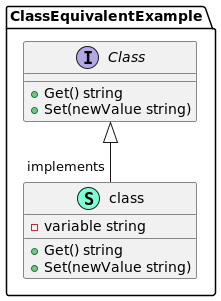
\includegraphics[height=0.3\textheight]{./part/Proyecto_ejecutivo/memoria_constructiva/ClassEquivalentInGolang}
    \caption{UML diagram: Class equivalent in Golang}\label{fig: uml Diagram Class Equivalent in Golang}
\end{figure}

por qué es importante concebir esta estructura:

\begin{itemize}
    \item Evitamos la instanciación no consistente, lo cual solo se garantiza a traves del método si exportado NewClass
    \item evitamos accesos no deseados al seteo de variables. Si las pusieramos publicas seria posible. esto es de vital importancia a la hora de establecer el concepto de inmutabilidad en la que se basan los value objects.
    \item otro punto de limpieza que aporta, es a la hora de gestionar errores en golang. Si en cualquier punto queremos devolver como resultado de una función un objeto o el error, característica de golang que permite devolver varios elementos como resultado, Nos veríamos obligados a instanciar el objeto con contenido vacío y el error, creando un elemento inconsistente sólo por exigencias del lenguaje. De esta forma, podemos poner como parámetro de retorno dicha interfaz que sí puede ser null.
\end{itemize}

como contrapartida tenemos que escribir más codigo. poniendo como comparación una clase java o C++ no podemos decir que en cantidad de lineas escritas se aumente o disminuya. En cuestión de conceptos aprendidos en Golang sólamente trabaja con interfaces y structs contra el concepto de clase y herencia.

Una vez presentado este concepto clave de golang pasamos a exponer el código que se ha ejecutado. Siendo programas extensos hemos decidido escoger el caso de uso más extenso el cuál incluye la gestión de los eventos y el proceso de intercomunicación. También expondremos expondremos el programa de control.

Vamos a dividir esta sección en:
\begin{itemize}
    \item CreateTaskUseCase
    \item TaskEventHandler
    \item TaskLooper
    \item CallAdapter
\end{itemize}

Que son los puntos que han presentado mayor complejidad.

\subsubsection{CreateTaskUseCase}
    
El codigo de colores utilizado en los diagramas de esta seccion se refieren al equivalente a clase en golang en azul y a las interfaces puras en turquesa  y a los structs en marron

%El tipico diagráma cuando se habla de arquitectura hexagonal es tal y como se muestra en la figura\ref{fig:hexagonalDiagram} Si bien consideramos que no tiene mucho sentido y de cara a la parte didáctica confunde, ya que el hexágono es una simple licencia estética. en el caso de existir más puertos de salida y entrada que los representados el hexágono pierde todo el sentido y cuando se enfrenta por primera vez este diagrama se tiende a intentar descifrar el sentído del hexagono.
%
%\begin{figure}[H]
%    \centering
%    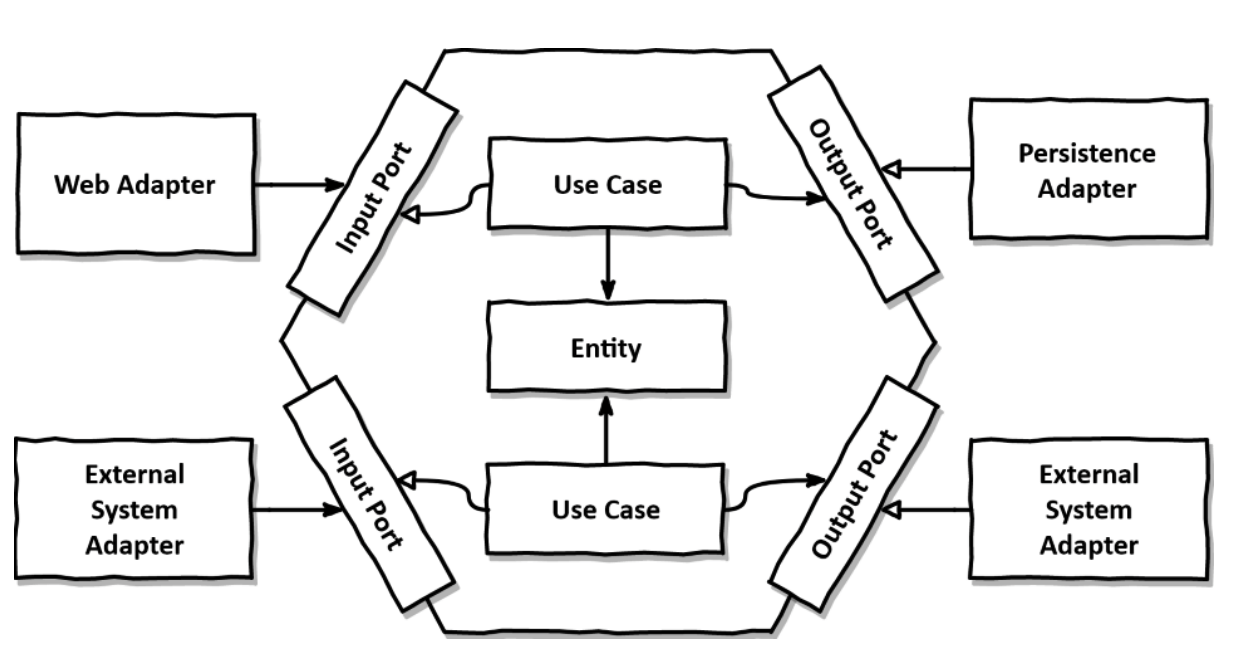
\includegraphics[height=0.3\textheight]{./part/Ejecucion/Seguimiento/CreateTaskUseCase/img/HexagonalDiagram}
%    \caption{Hexagonal architecture diagram\cite{TomHombergs2019GYHD}}\label{fig:hexagonalDiagram}
%\end{figure}

Tomando como referencia \ref{fig:hexagonalDiagram} el diagrmaa tipico de una arquitectura hexagonal, en nuestro caso si intercambiamos ExternalSystemAdapter por nuestro Dispatcher de eventos e introducimos servicios de dominio entre el caso de uso y la Entidad tendremos nuestro esquema de alto nivel de nuestra arquitectura hexagonal. El esbozo de este diagrama lo podemos encontrar en la figura\ref{fig:CreateTaskHexagonalDiagram} Como vemos no tiene tanto sentido el dibujo ya que hay puertos de salida que se convierten en puertos de entrada como es el dispatcher y cuando queremos quitar lógica de negocio del caso de uso mediante servicios de dominio que impidan el acceso directo a los repositorios de persistencia dicho diagrama se va quedando pequeño. Es perferible diagramas UML tal y comose muestra en\ref{fig:createTaskUseCaseArchitecture}


\begin{figure}[H]
    \centering
    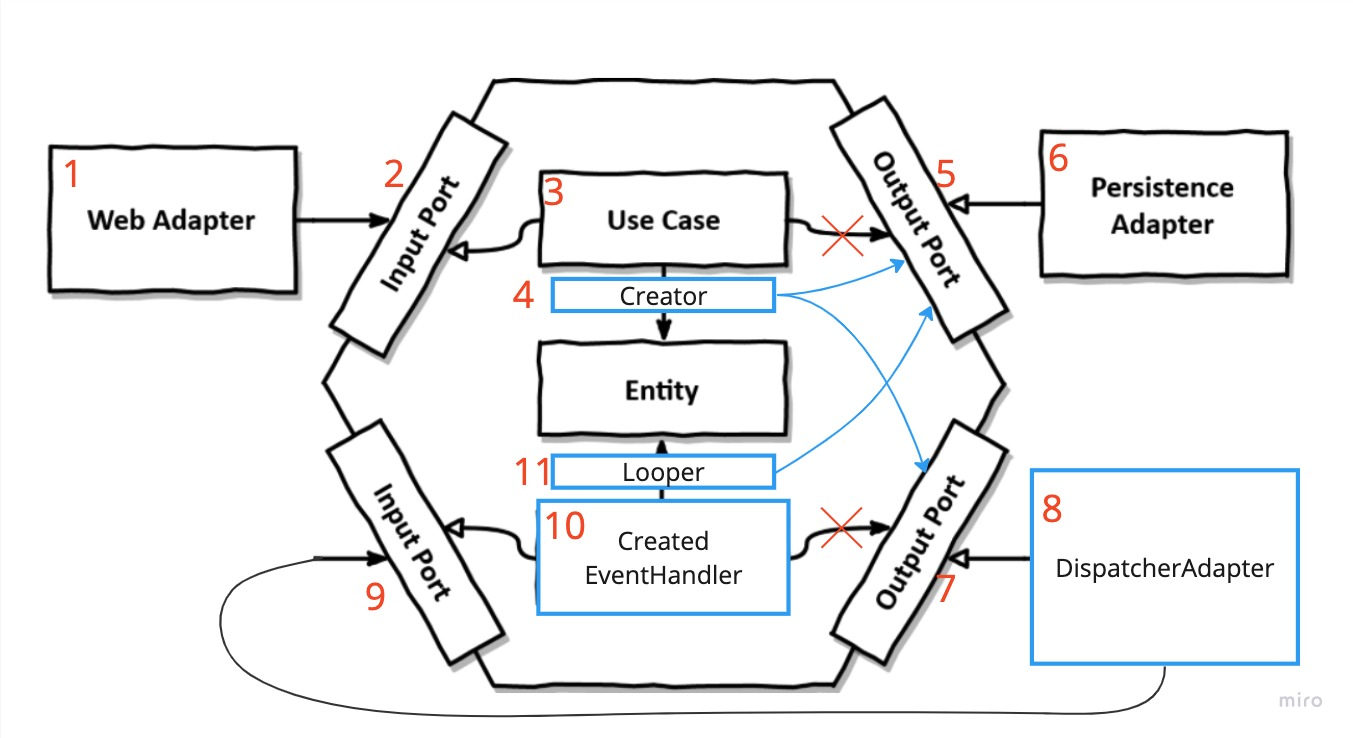
\includegraphics[height=0.3\textheight]{./part/Ejecucion/Seguimiento/CreateTaskUseCase/img/CreateTaskHexagonalDiagram}
    \caption{Hexagonal architecture diagram}\label{fig:CreateTaskHexagonalDiagram}
\end{figure}

\begin{figure}[H]
    \centering
    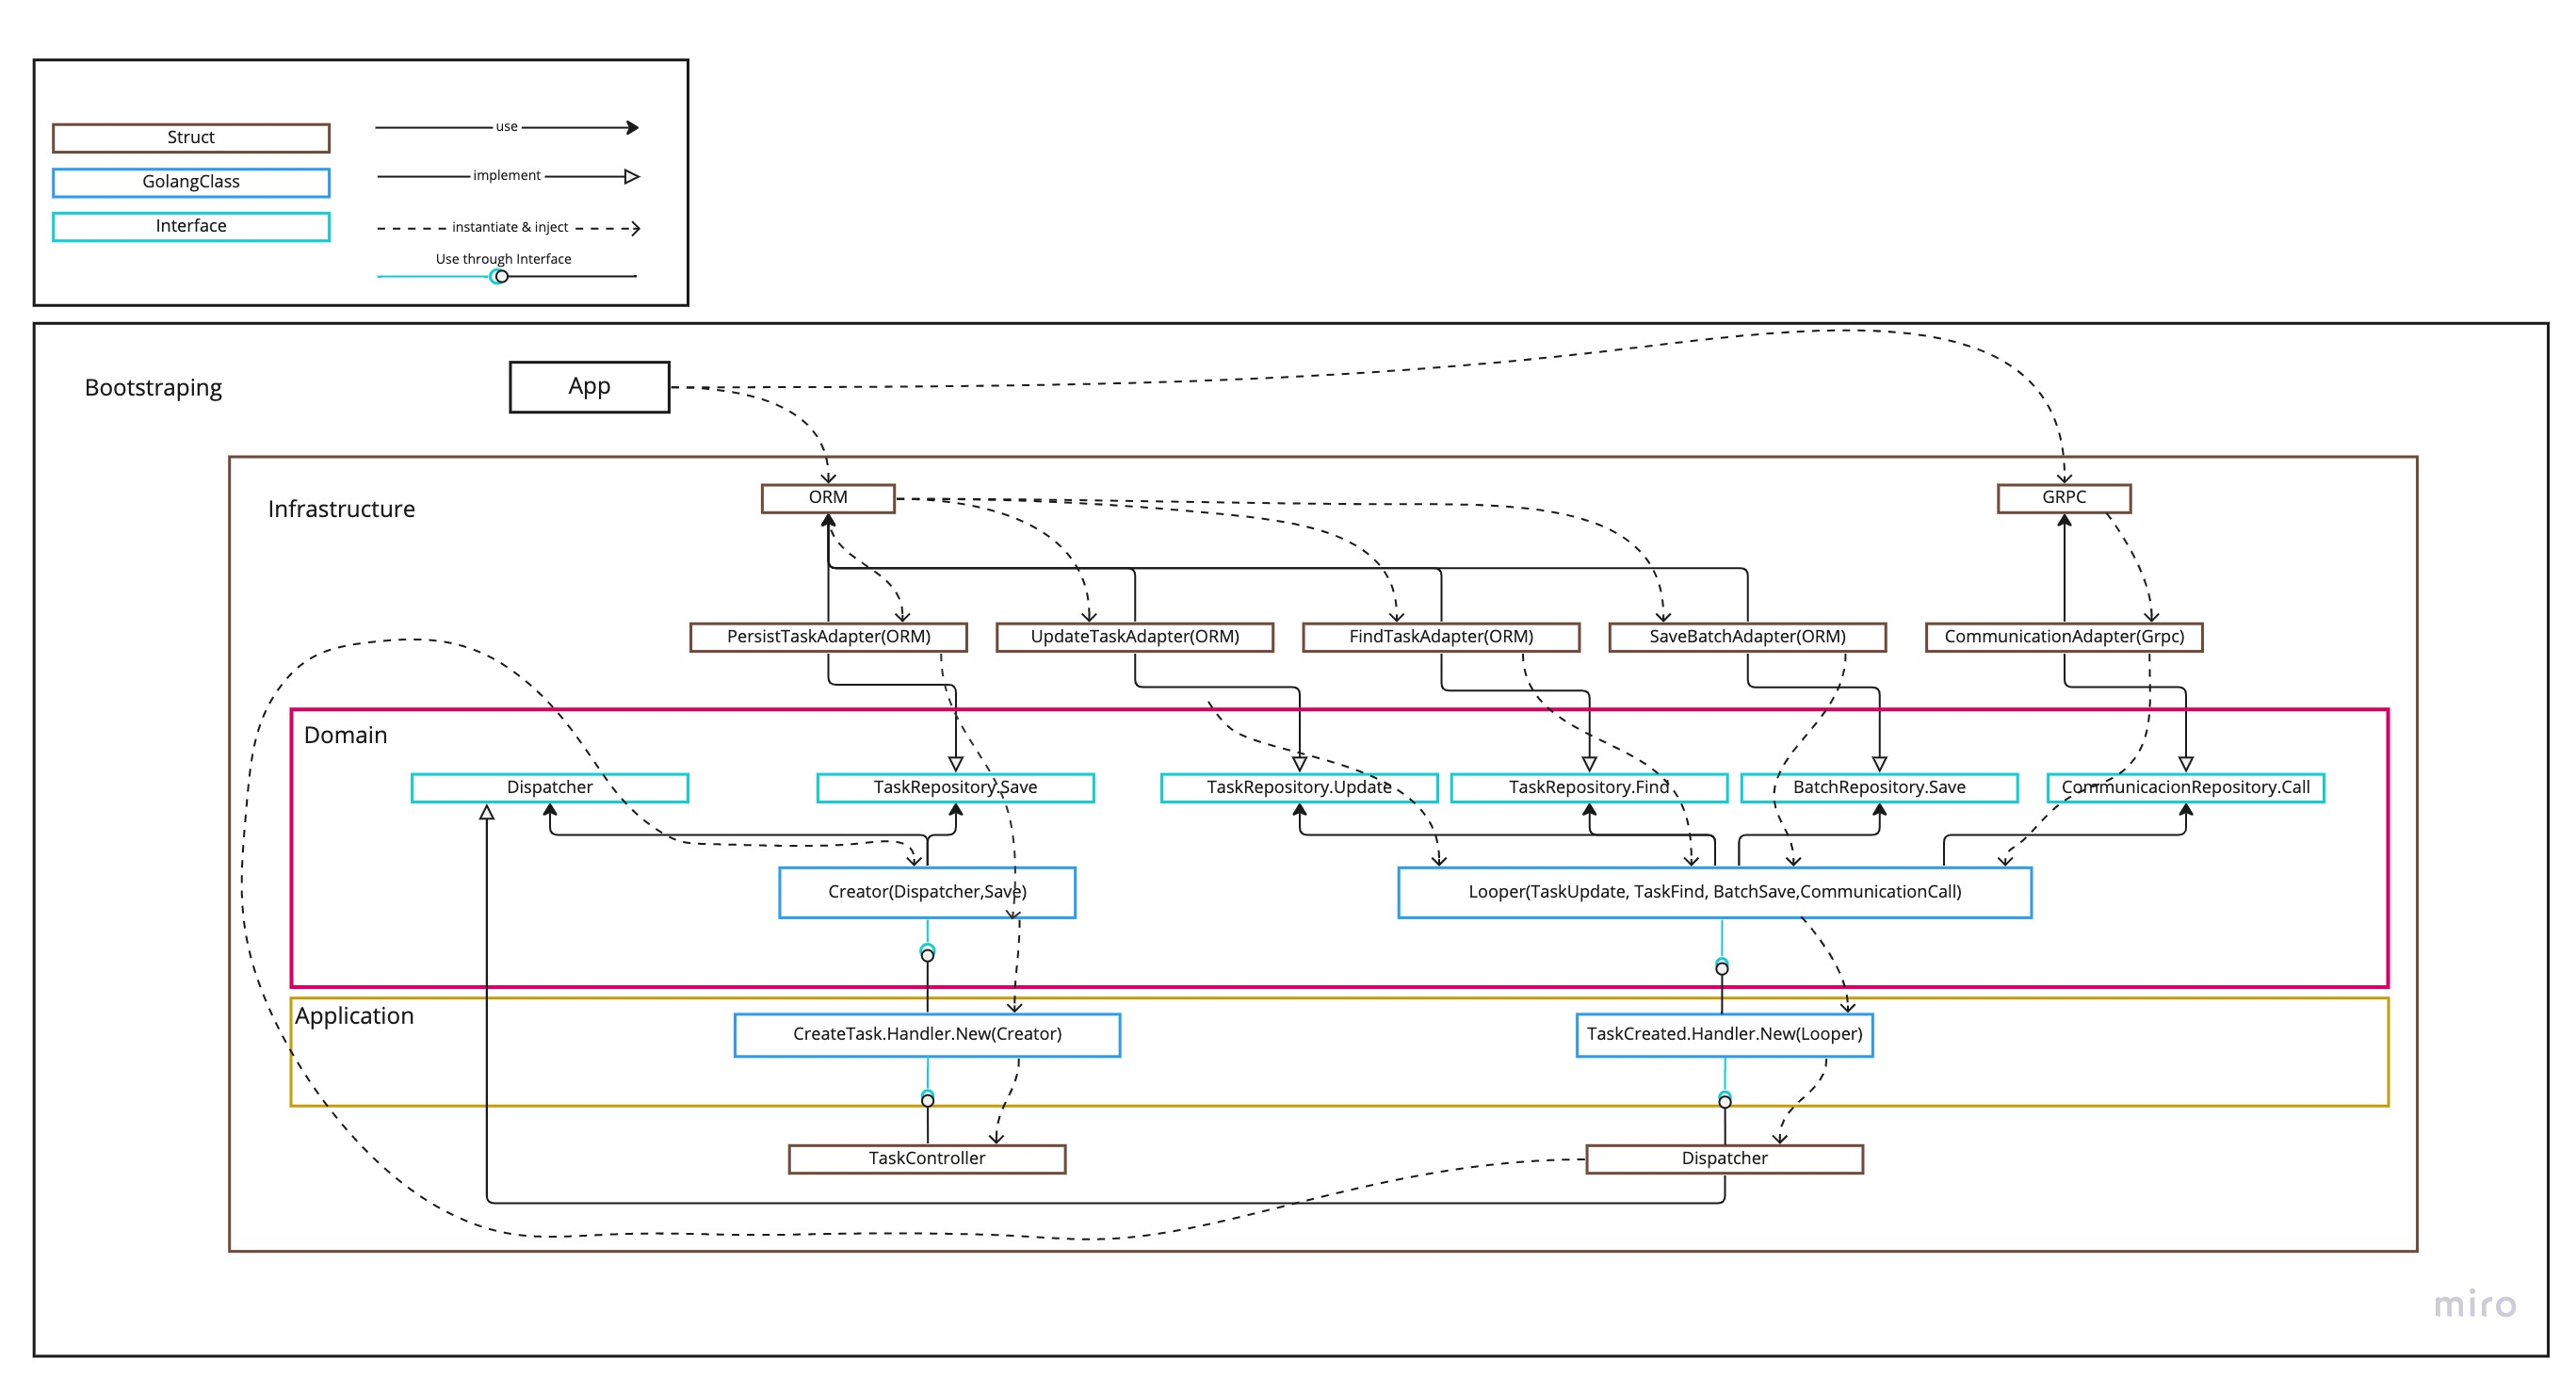
\includegraphics[height=0.3\textheight]{./part/Ejecucion/Seguimiento/CreateTaskUseCase/img/createTaskUseCaseArchitecture}
    \caption{CreateTaskUseCase hexagonal architecture diagram}\label{fig:createTaskUseCaseArchitecture}
\end{figure}

Acercandonos más al código podemos ver en el diagrama \ref{fig:createTaskUseCaseArchitectureFolderStructure} cómo es el uso entre los componentes que exísten en la estructrura de carpetas.

\begin{figure}[H]
    \centering
    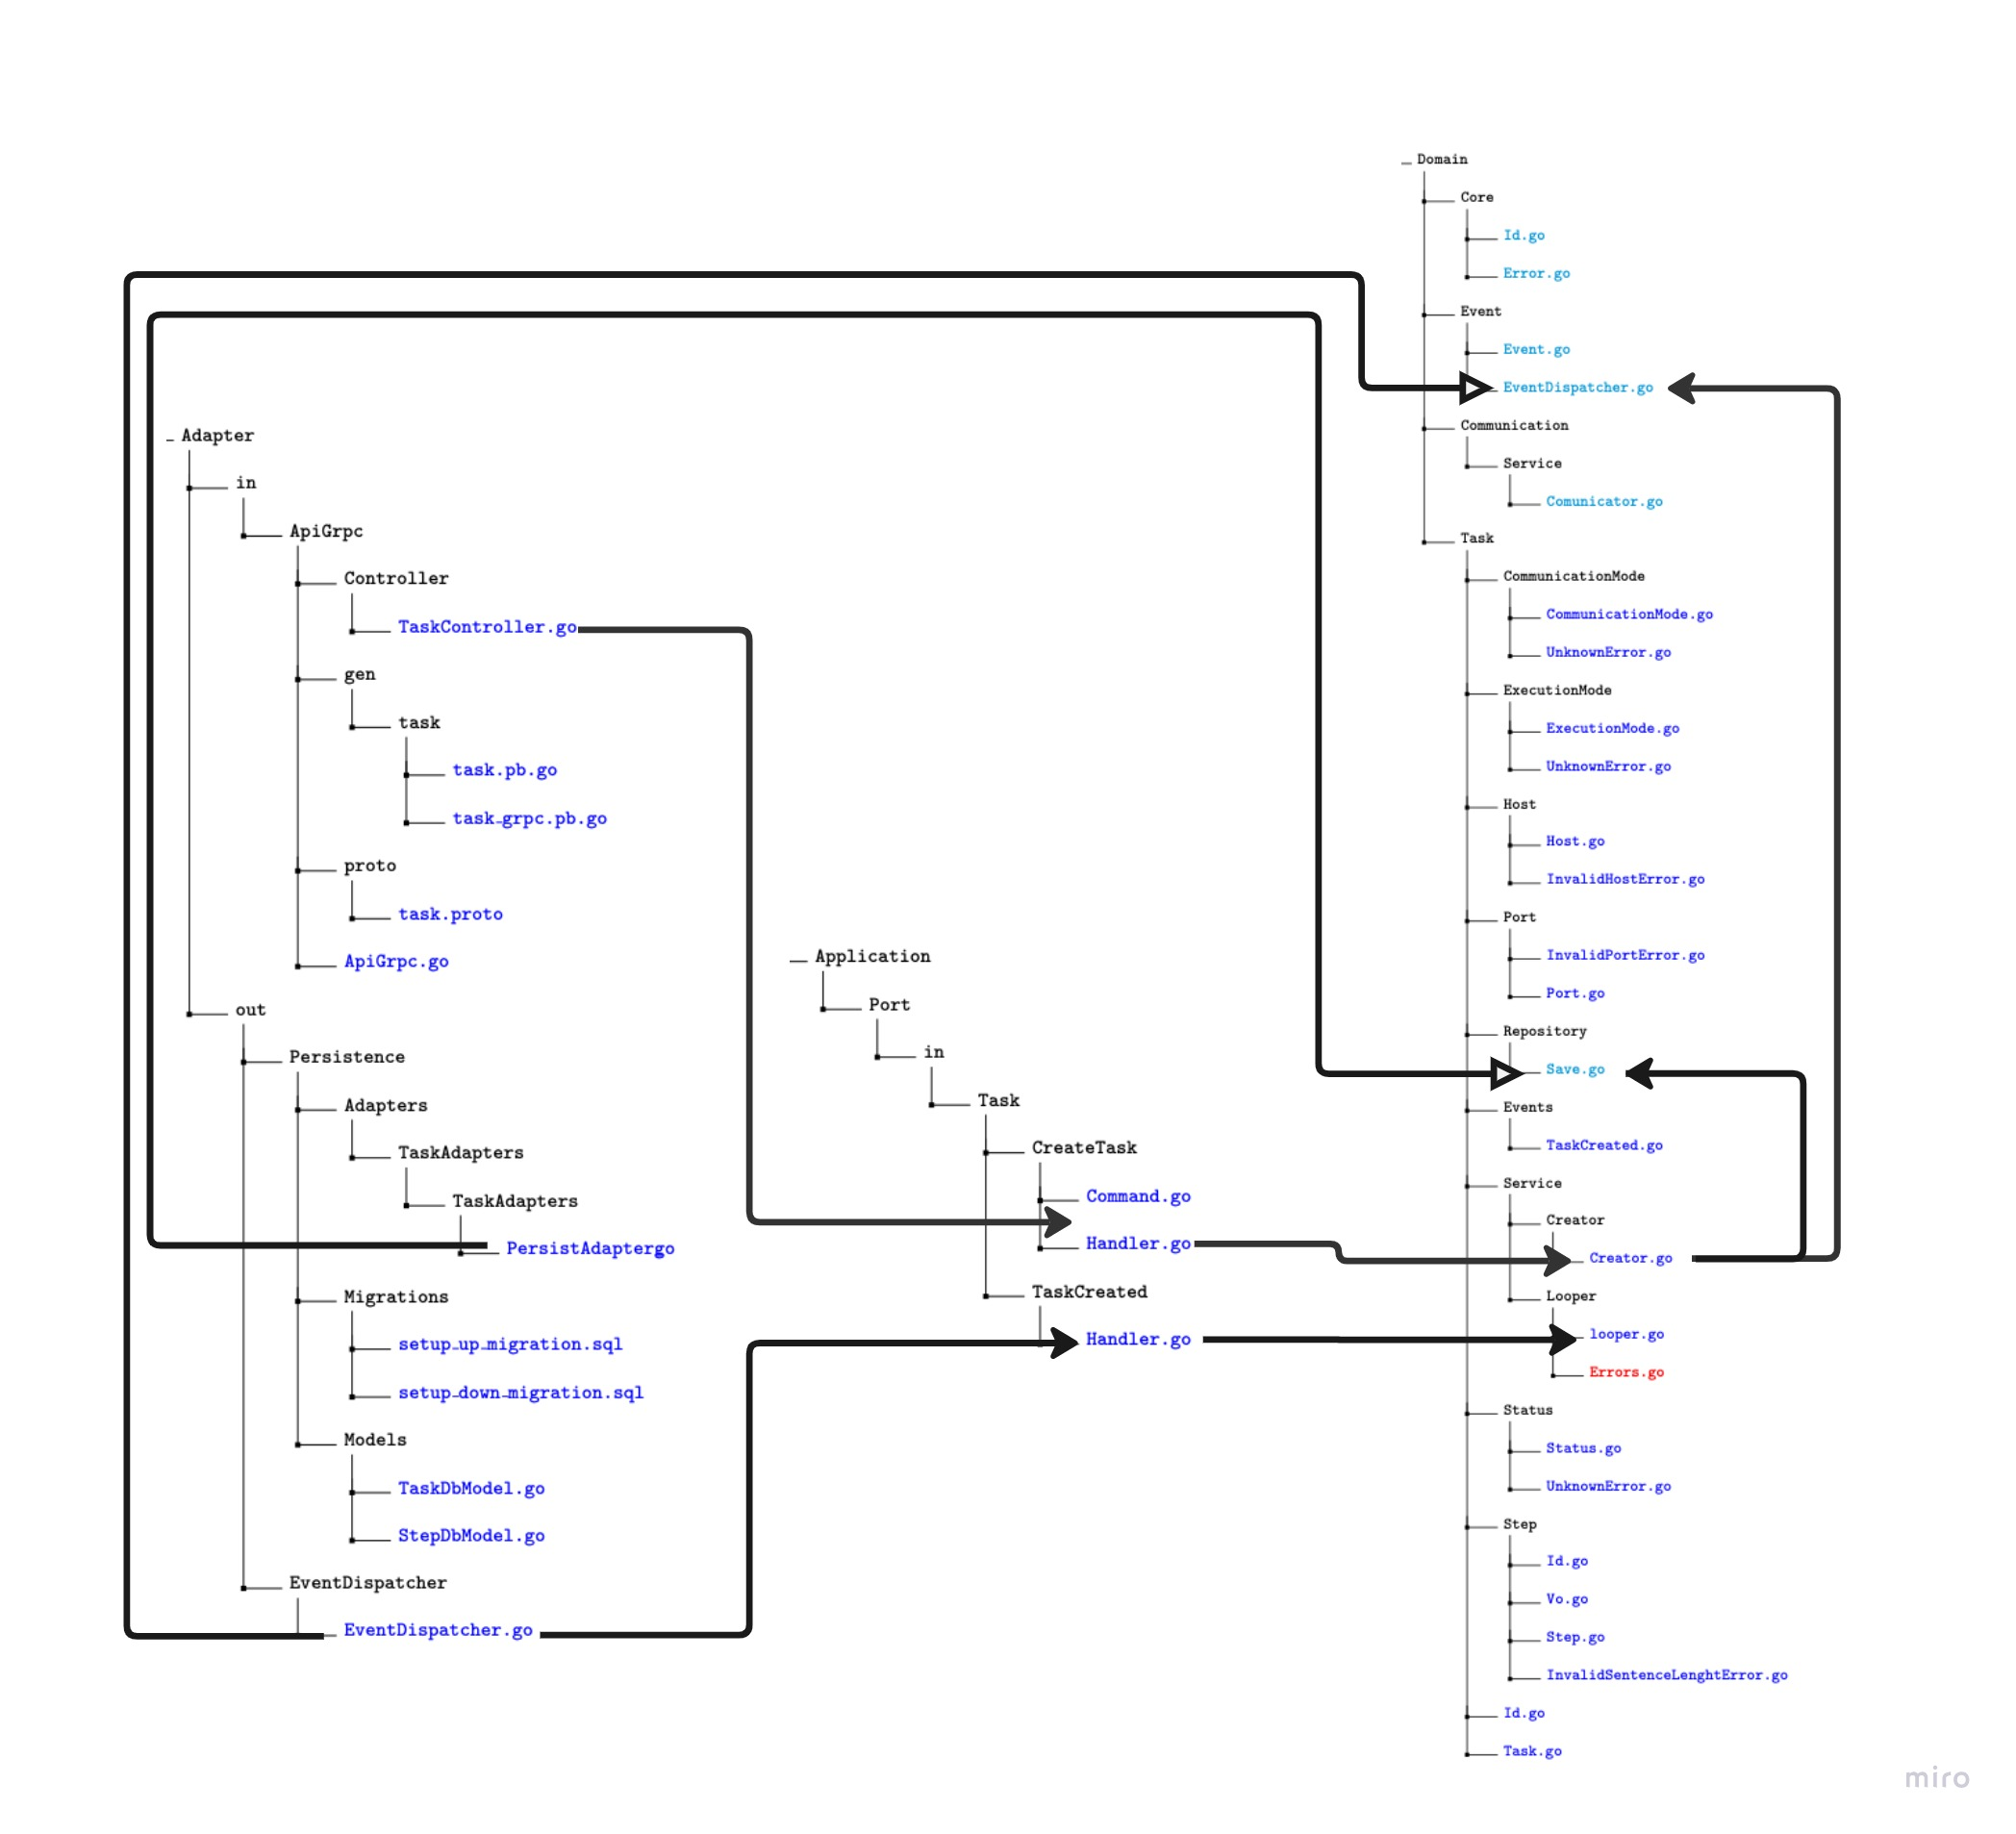
\includegraphics[height=0.5\textheight]{./part/Ejecucion/Seguimiento/CreateTaskUseCase/img/PFM - CreateUseCaseFolderStructure}
    \caption{CreateTaskUseCase folder Structure}\label{fig:createTaskUseCaseArchitectureFolderStructure}
\end{figure}

%Un punto interesante a comentar es el concepto de la estrategia de mapping que hay entre capas. Cada capa requiere sus objetos de trabajo. Tal y como sale descrito en \cite{TomHombergs2019GYHD} Tenemos tantas estratégias como atajos dentro de este paradigma queramos asumir. podemos ver en la figura \ref{fig:mapping types} Los tipos de mapping que se documentan en este libro:
%\begin{itemize}
%    \item The NoMapping Strategy
%    \item The Two-Way MappingStrategy
%    \item The Full MappingStrategy
%    \item The One-Way MappingStrategy
%\end{itemize}

Con respecto a la estrategia de mapping Golang nos permite hacer un full strategy casi por defecto porque al necesitar la implementaci'on de clase para garantizar la cohesión ya estamos utilizando interfaces para todas las clases. Así que en este caso utilizamos un fullMapping adaptado. lo cierto es que las versiones intermedias son todas las combinaciones posibles.

De cara a decidir extraemos la recomendacion de  \cite{TomHombergs2019GYHD}:"
we might start with a simple strategy that allows us to quickly evolve the code and later move to a more complex one that helps us to better decouple the layers.
In order to decide which strategy to use when, we need to agree upon a set of guidelines within the team. These guidelines should answer the question which mapping strategy should be the first choice in which situation. They should also answer why they are first choice so that we’re able to evaluate if those reasons still apply after some time."

Al final se trata de tomar una decisión en equipo, documentar las razones y ser consistentes. Reevaluar las razones ante un reto que las ponga a prueba y tomar o no la decisión de cambiar la estrategia.

En nuestra opinión dentro de la estrategia fullmapping se debe implementar un modelo tanto de entrada, como ya se contempla, como de salída. Es decir, la respuesta que hay entre cada capa también debe ser mappeada, podemos ver el patrón readptado en la figura \ref{fig:GetHandMapping}

\begin{figure}[H]
    \centering
    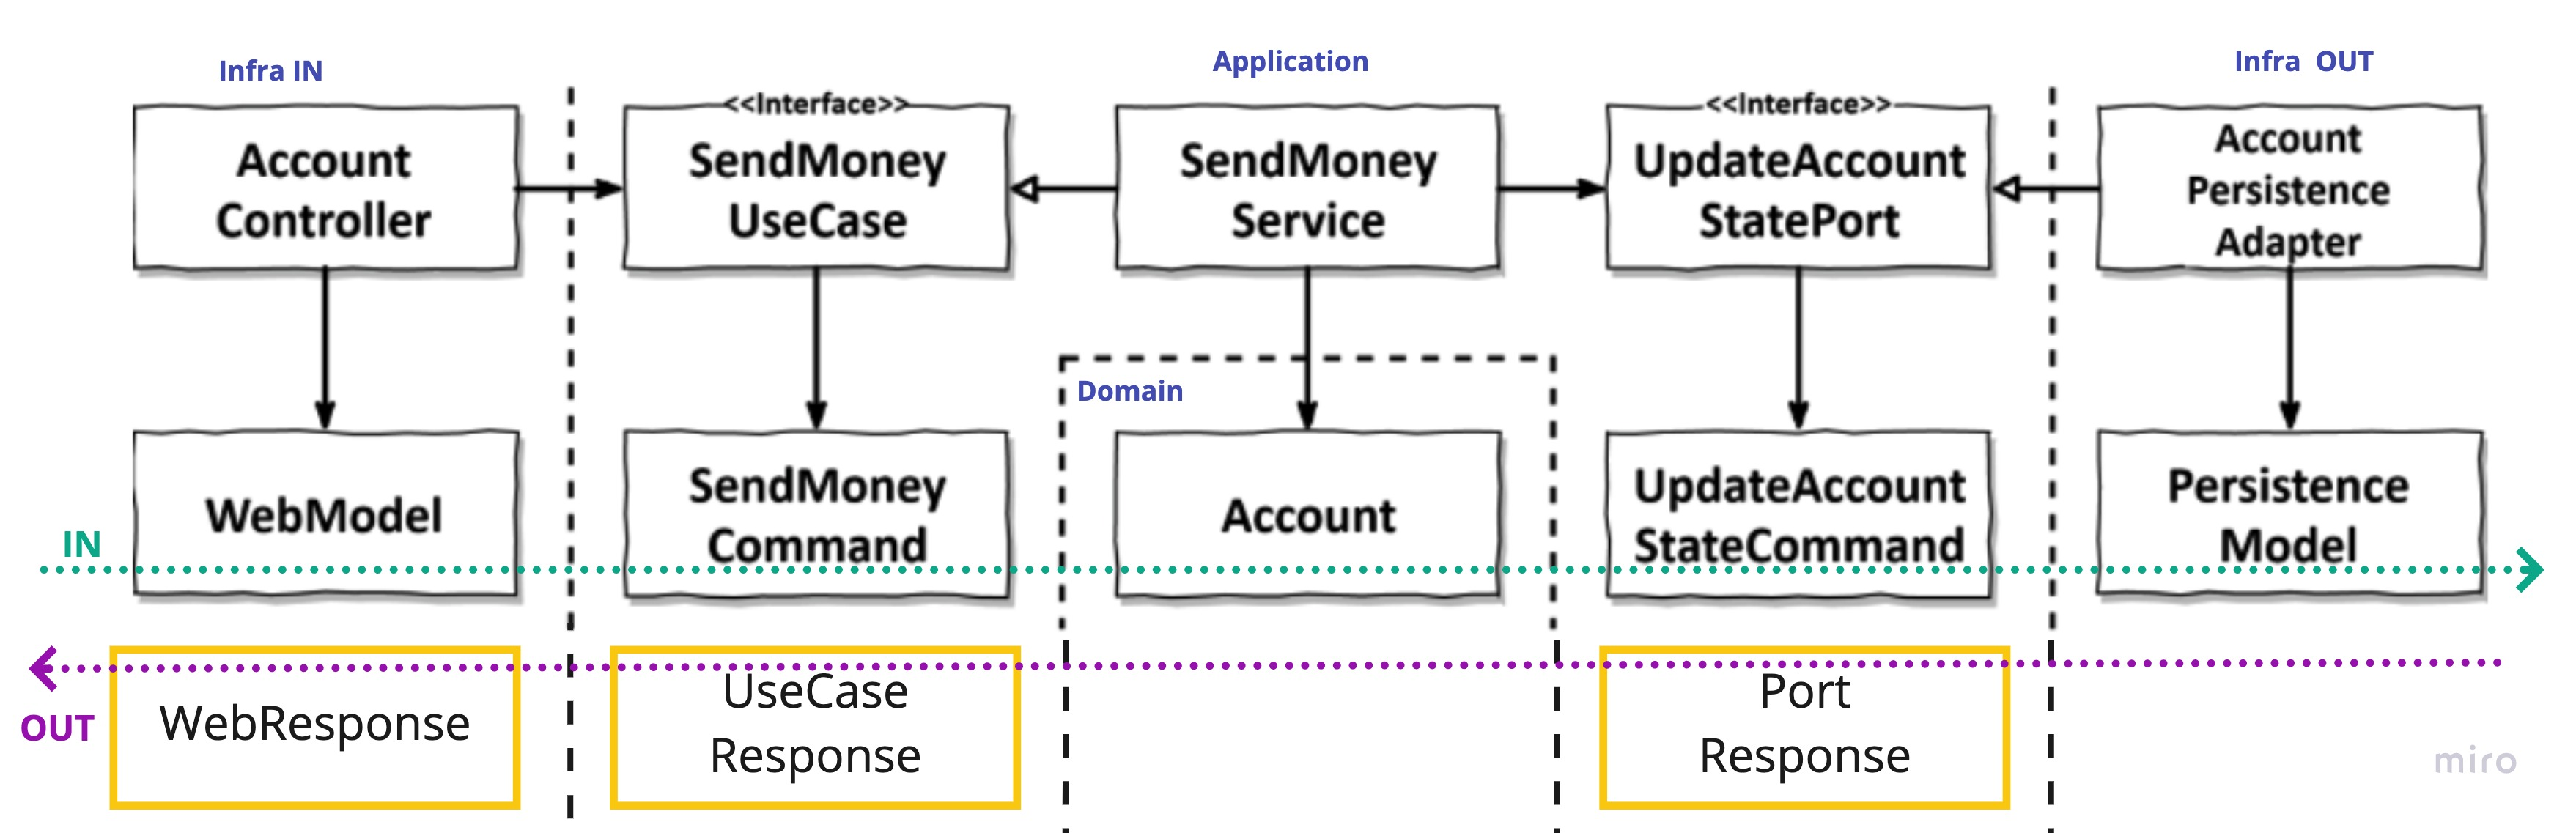
\includegraphics[height=0.2\textheight]{./part/Ejecucion/Seguimiento/CreateTaskUseCase/img/PFM - GetHandMapping}
    \caption{CreateTaskUseCase folder Structure\cite{TomHombergs2019GYHD}}\label{fig:GetHandMapping}
\end{figure}

Claramente esto aumenta la burocracia y finalmente la opción que hemos tomado se puede ver en la figura\ref{fig:CreateTaskUseCaseMapping}

En rojo se han marcado los atajos que se han tomado, es decir, el mapeo que no se ha implementado. El objetivo es aislarse bien de los puertos de entrada, es decir el GRPC, y no tanto de los puertos de salida. ya que la persistencia está bien aislada mediante las interfaces. Dentro de los adaptadores se hará el trabajo de mappeo entre las entidades de dominio y los modelos de persistencia y se traducirá de nuevo a dominio para responder.

\begin{figure}[H]
    \centering
    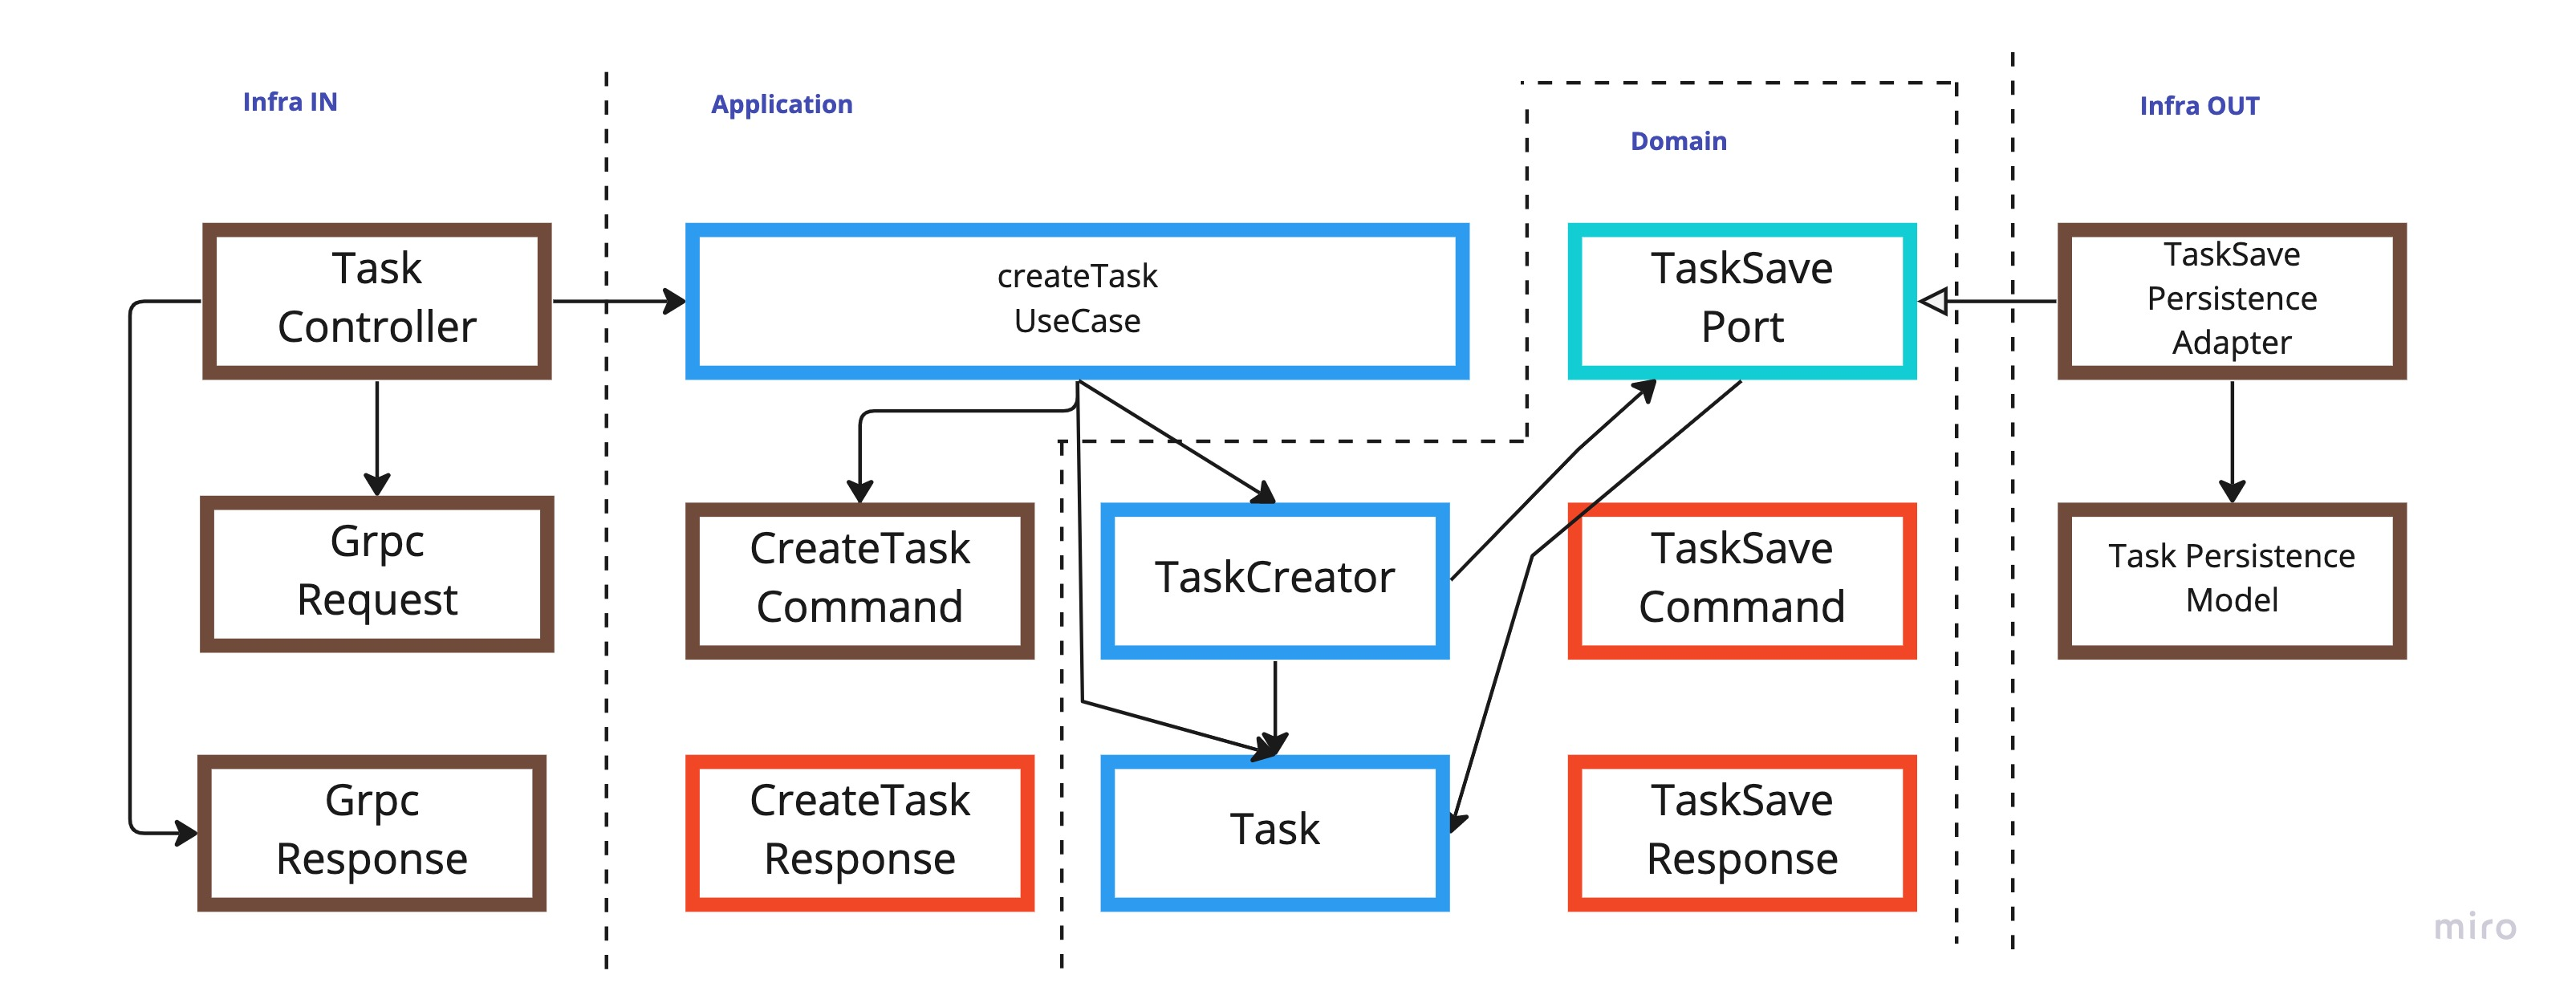
\includegraphics[height=0.2\textheight]{./part/Ejecucion/Seguimiento/CreateTaskUseCase/img/PFM - FinalMapping}
    \caption{CreateTaskUseCase folder Structure}\label{fig:CreateTaskUseCaseMapping}
\end{figure}

Ahora vamos a exponer el código final de este caso de uso, vamos a hacer referencia a:
\begin{itemize}
    \item TaskController \ref{fig:TaskControler}
    \item CreateTaskUseCase \ref{fig:CreateTaskUseCaseCode}
    \item Creator \ref{fig:Creator}
    \item SavePort \ref{fig:SavePort}
    \item PersistAdapter \ref{fig:SaveAdapter}
    \item DispatcherPort \ref{fig:DispatcherPort}
\end{itemize}

\begin{figure}[H]
    \centering
    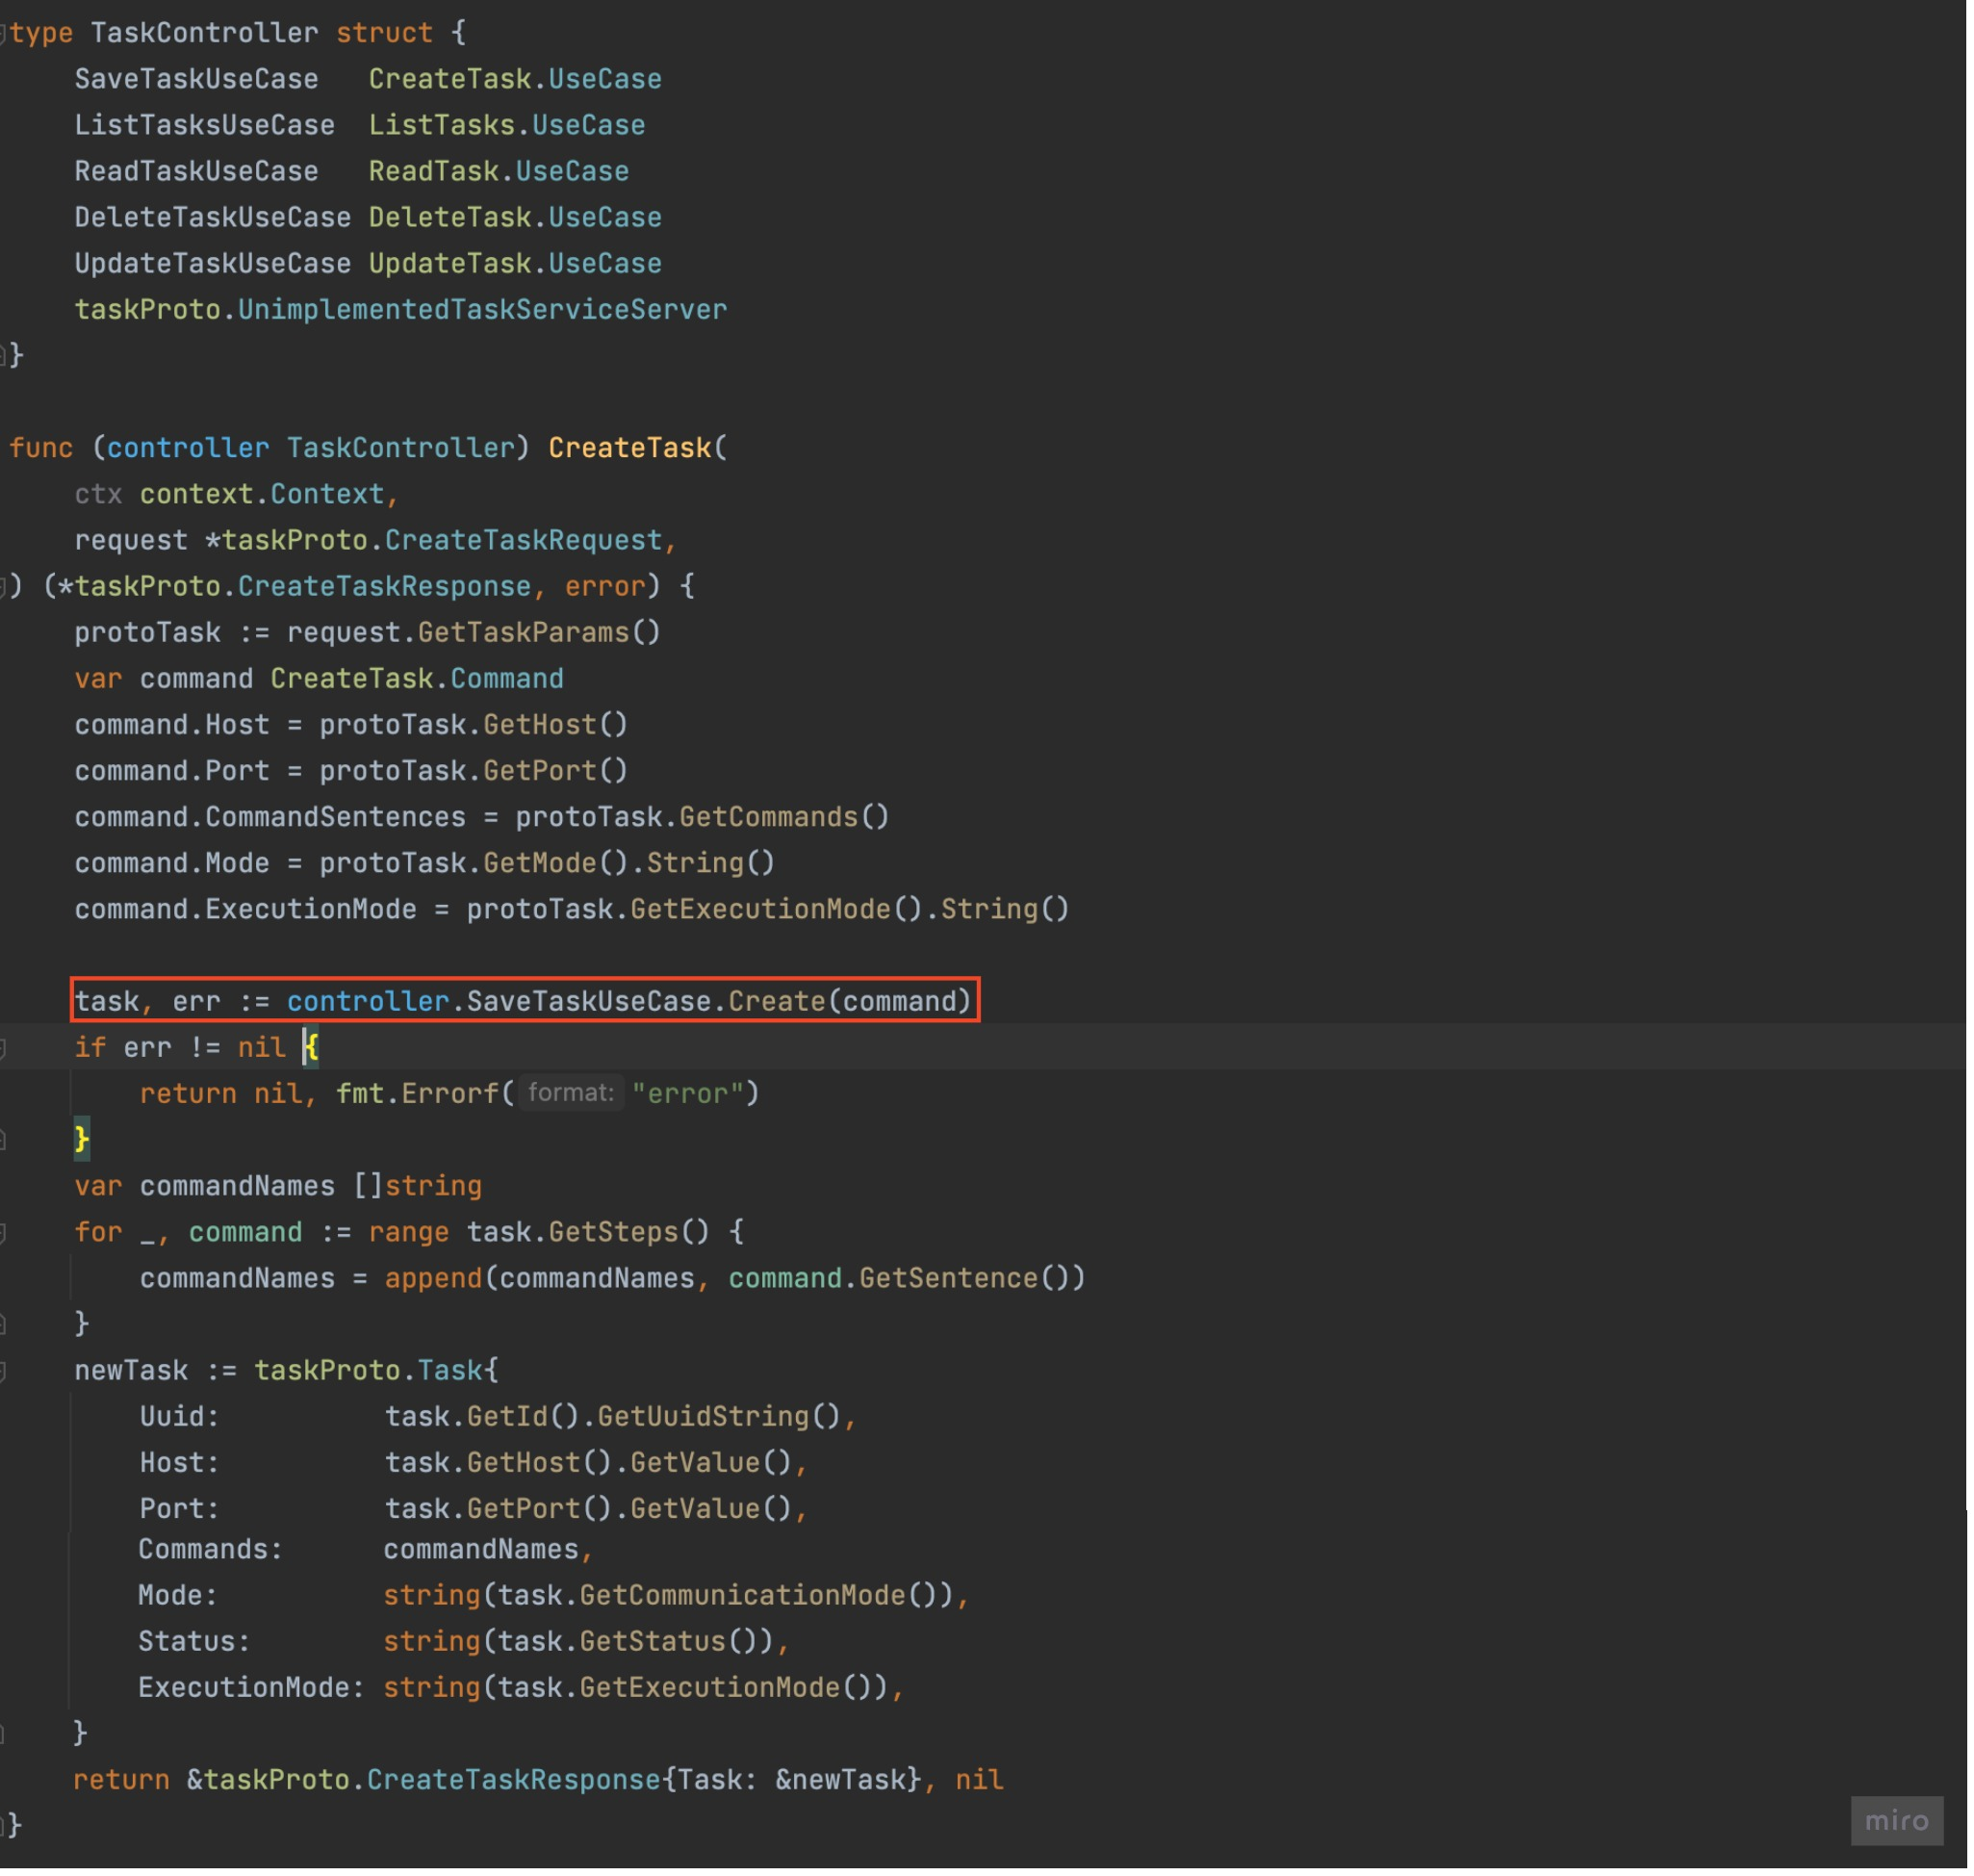
\includegraphics[height=0.5\textheight]{./part/Ejecucion/Seguimiento/CreateTaskUseCase/img/PFM - TaskController}
    \caption{TaskController.go}\label{fig:TaskControler}
\end{figure}

\begin{figure}[H]
    \centering
    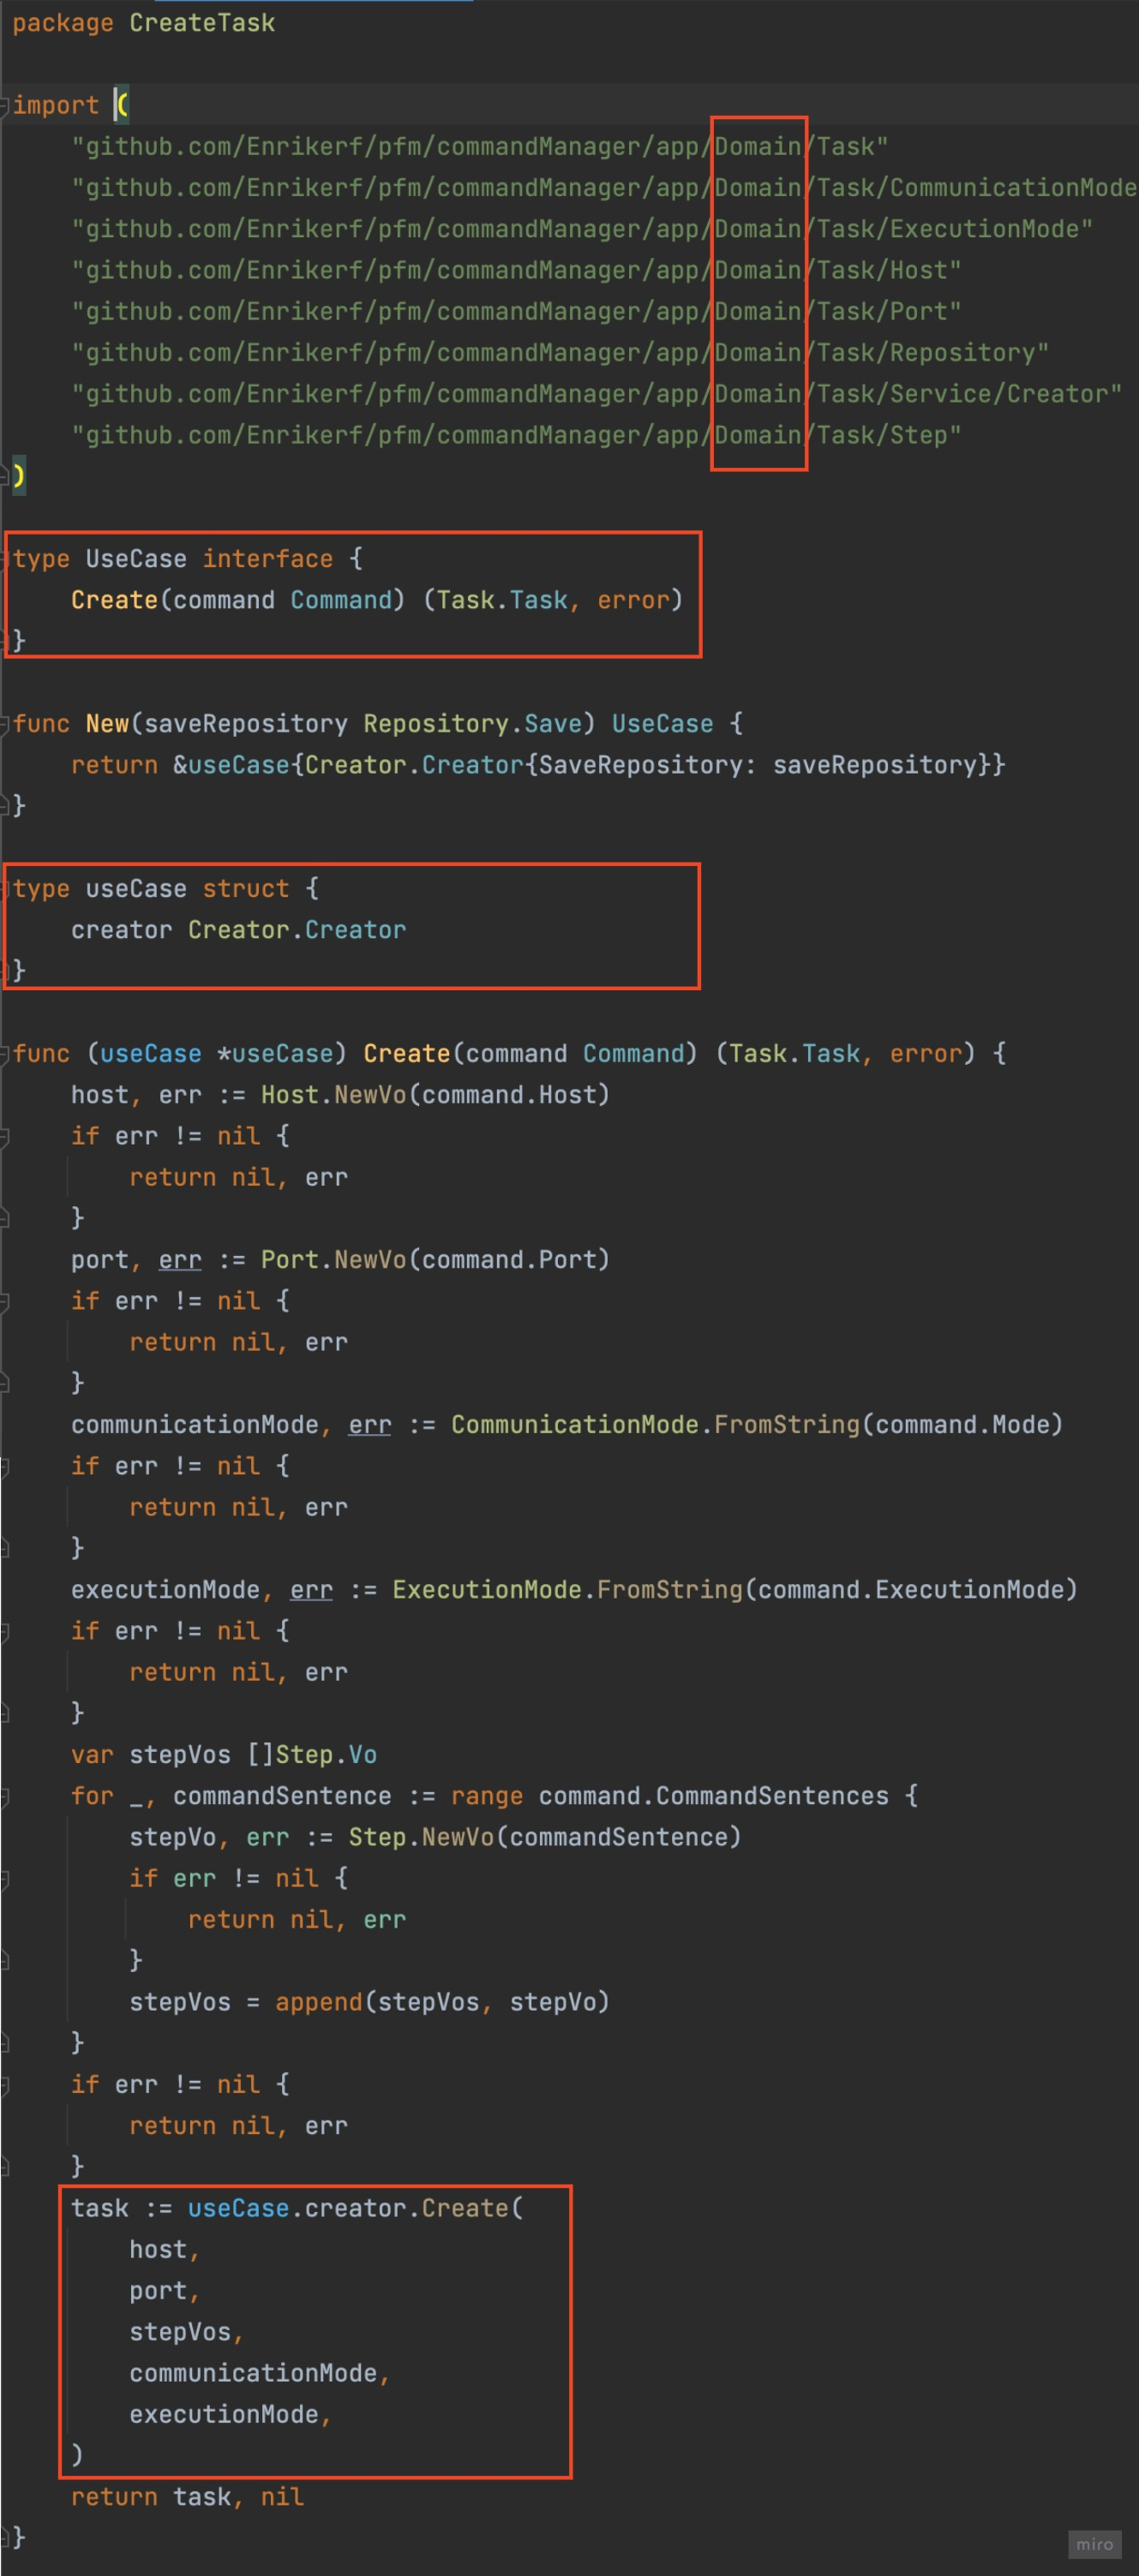
\includegraphics[height=0.5\textheight]{./part/Ejecucion/Seguimiento/CreateTaskUseCase/img/PFM - CreateTaskUseCaseCode}
    \caption{CreateTaskUseCaseCode.go}\label{fig:CreateTaskUseCaseCode}
\end{figure}

\begin{figure}[H]
    \centering
    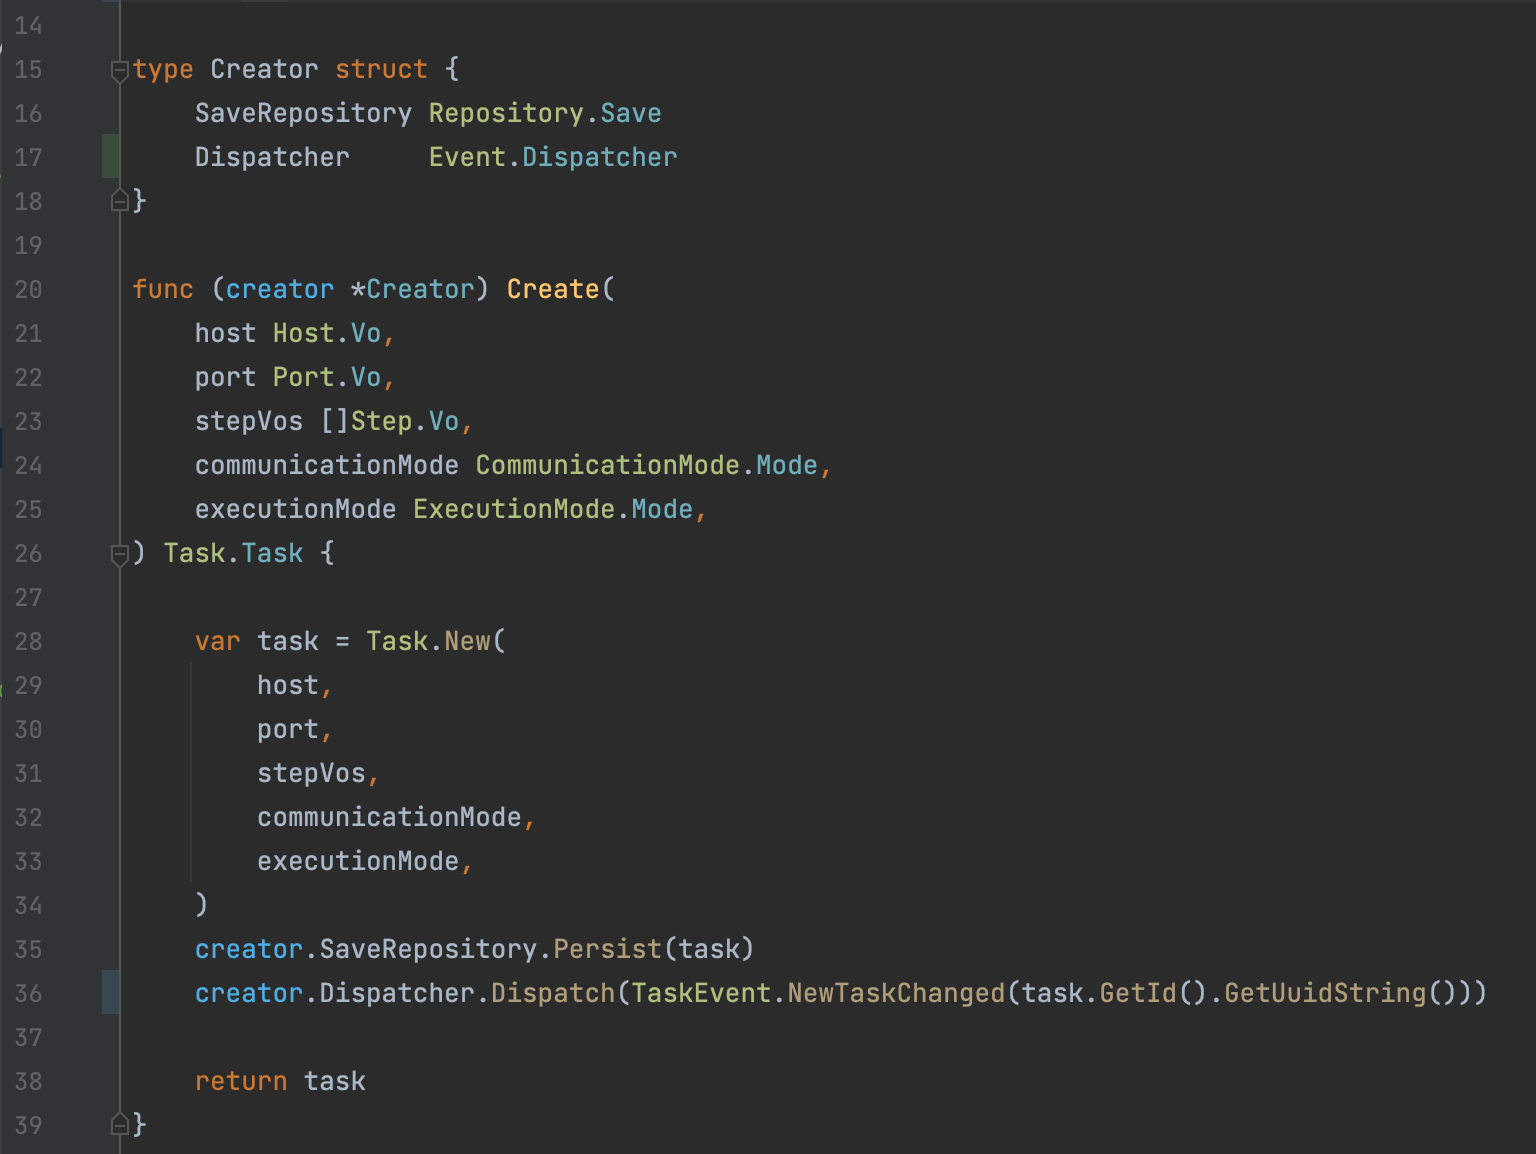
\includegraphics[height=0.5\textheight]{./part/Ejecucion/Seguimiento/CreateTaskUseCase/img/PFM - creator}
    \caption{Creator.go}\label{fig:Creator}
\end{figure}

\begin{figure}[H]
    \centering
    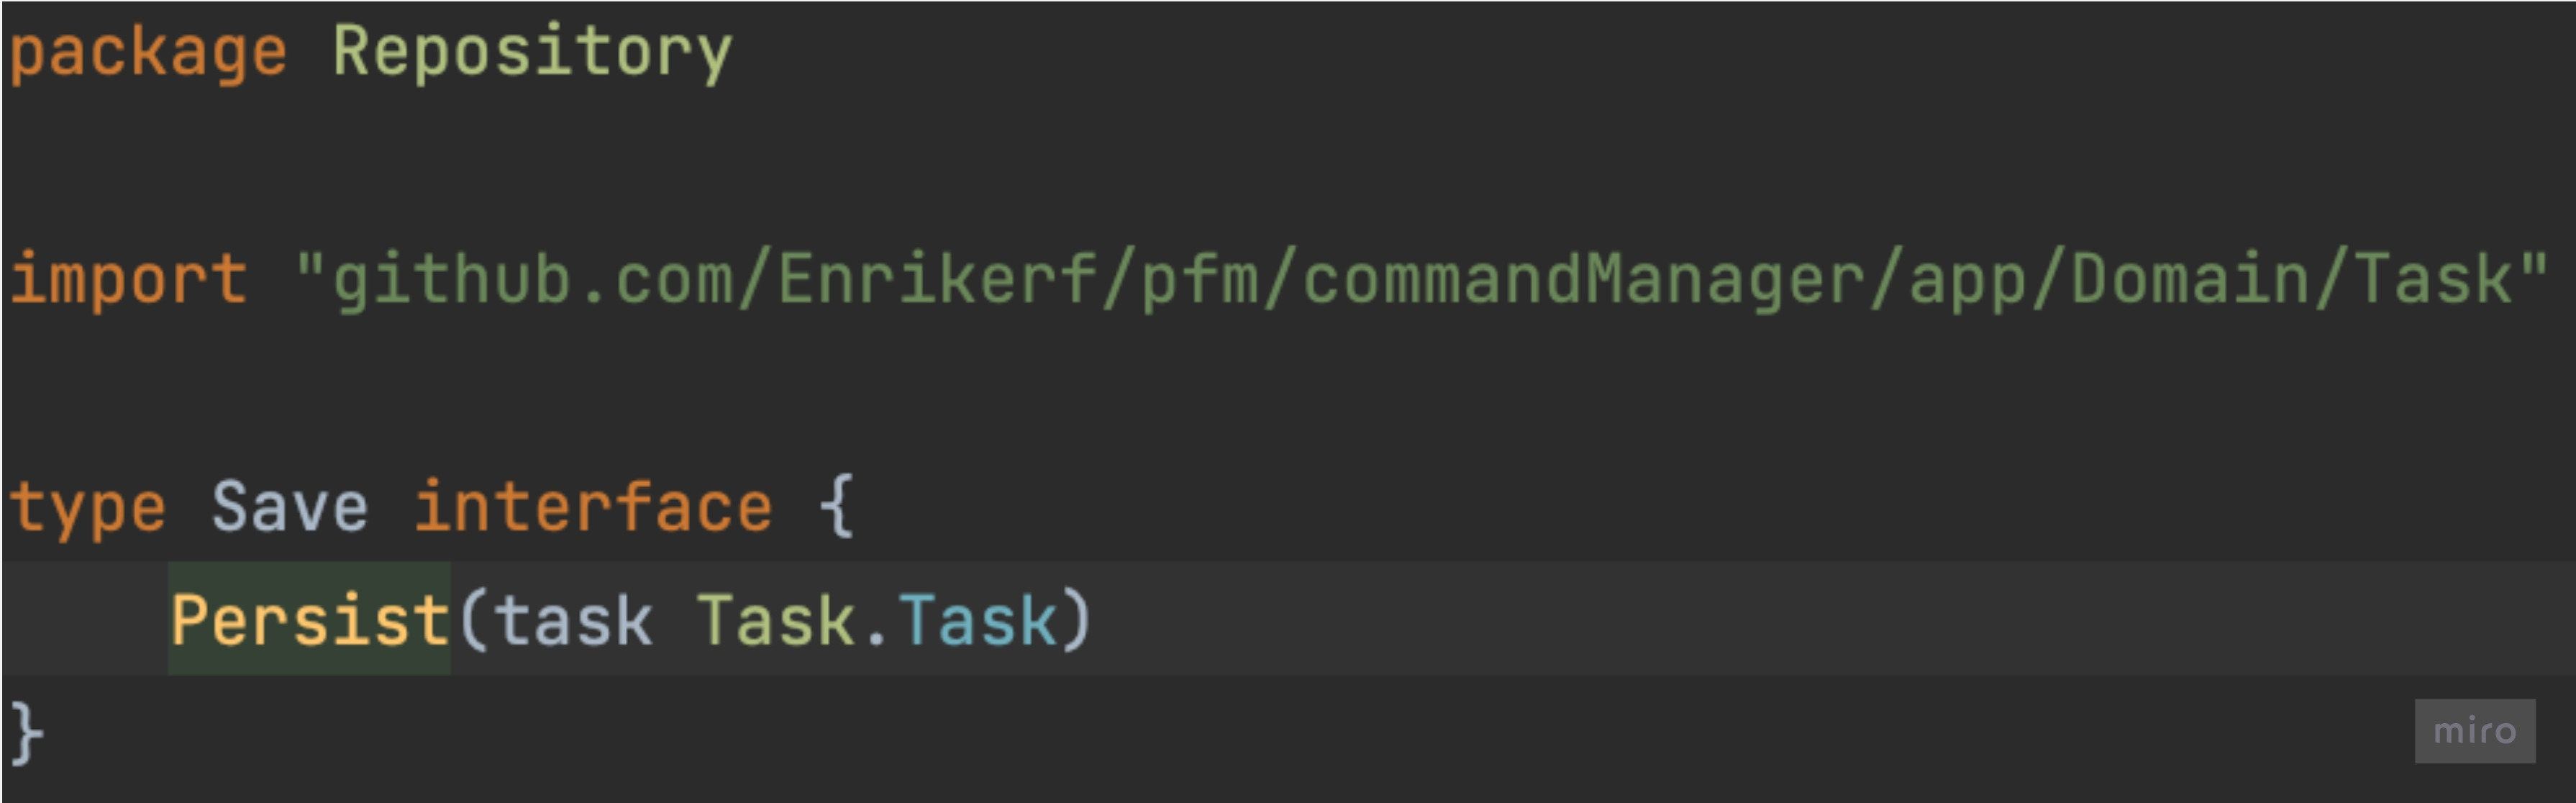
\includegraphics[height=0.2\textheight]{./part/Ejecucion/Seguimiento/CreateTaskUseCase/img/PFM - SavePort}
    \caption{Creator.go}\label{fig:SavePort}
\end{figure}

\begin{figure}[H]
    \centering
    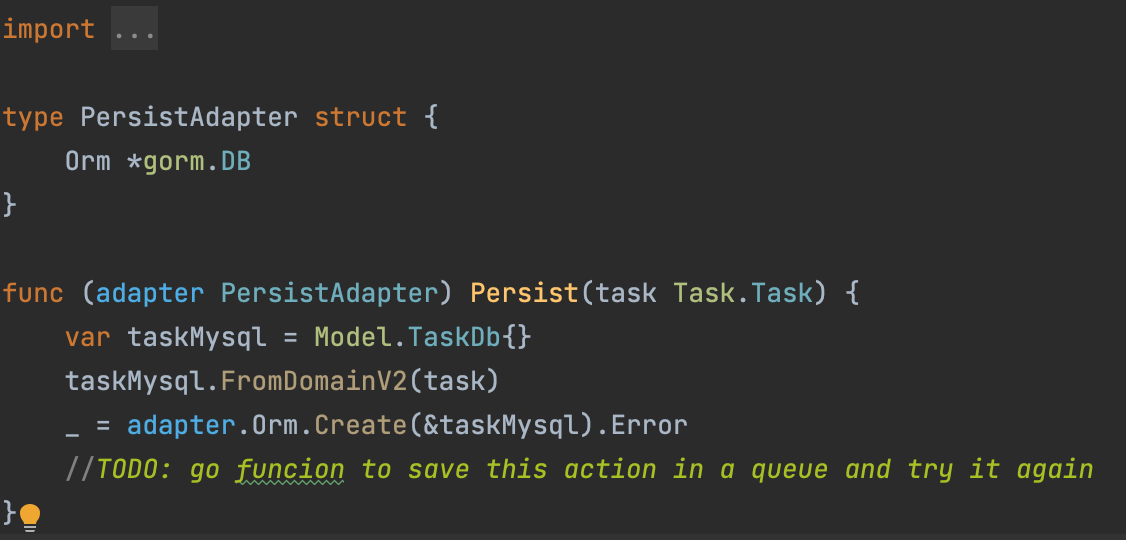
\includegraphics[height=0.2\textheight]{./part/Ejecucion/Seguimiento/CreateTaskUseCase/img/PFM - SaveAdapter}
    \caption{Creator.go}\label{fig:SaveAdapter}
\end{figure}

\begin{figure}[H]
    \centering
    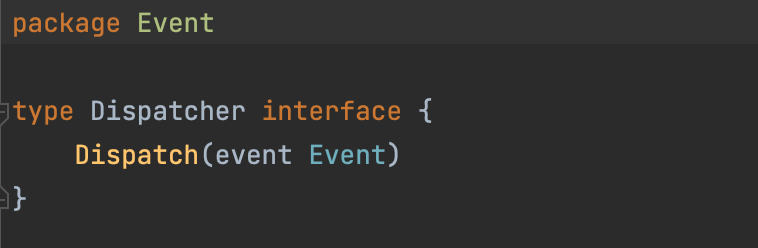
\includegraphics[height=0.2\textheight]{./part/Ejecucion/Seguimiento/CreateTaskUseCase/img/PFM - Dispatcher}
    \caption{Creator.go}\label{fig:DispatcherPort}
\end{figure}
\subsubsection{TaskEventHandler}
%    
El codigo de colores utilizado en los diagramas de esta seccion se refieren al equivalente a clase en golang en azul y a las interfaces puras en turquesa  y a los structs en marron

%El tipico diagráma cuando se habla de arquitectura hexagonal es tal y como se muestra en la figura\ref{fig:hexagonalDiagram} Si bien consideramos que no tiene mucho sentido y de cara a la parte didáctica confunde, ya que el hexágono es una simple licencia estética. en el caso de existir más puertos de salida y entrada que los representados el hexágono pierde todo el sentido y cuando se enfrenta por primera vez este diagrama se tiende a intentar descifrar el sentído del hexagono.
%
%\begin{figure}[H]
%    \centering
%    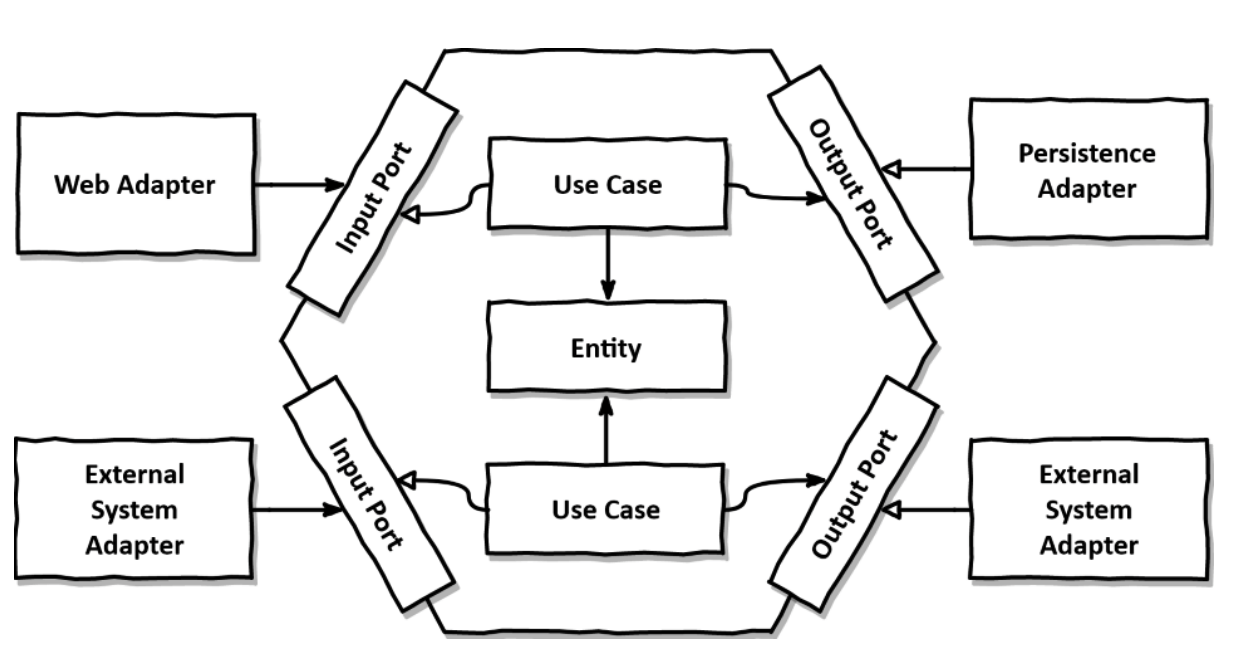
\includegraphics[height=0.3\textheight]{./part/Ejecucion/Seguimiento/CreateTaskUseCase/img/HexagonalDiagram}
%    \caption{Hexagonal architecture diagram\cite{TomHombergs2019GYHD}}\label{fig:hexagonalDiagram}
%\end{figure}

Tomando como referencia \ref{fig:hexagonalDiagram} el diagrmaa tipico de una arquitectura hexagonal, en nuestro caso si intercambiamos ExternalSystemAdapter por nuestro Dispatcher de eventos e introducimos servicios de dominio entre el caso de uso y la Entidad tendremos nuestro esquema de alto nivel de nuestra arquitectura hexagonal. El esbozo de este diagrama lo podemos encontrar en la figura\ref{fig:CreateTaskHexagonalDiagram} Como vemos no tiene tanto sentido el dibujo ya que hay puertos de salida que se convierten en puertos de entrada como es el dispatcher y cuando queremos quitar lógica de negocio del caso de uso mediante servicios de dominio que impidan el acceso directo a los repositorios de persistencia dicho diagrama se va quedando pequeño. Es perferible diagramas UML tal y comose muestra en\ref{fig:createTaskUseCaseArchitecture}


\begin{figure}[H]
    \centering
    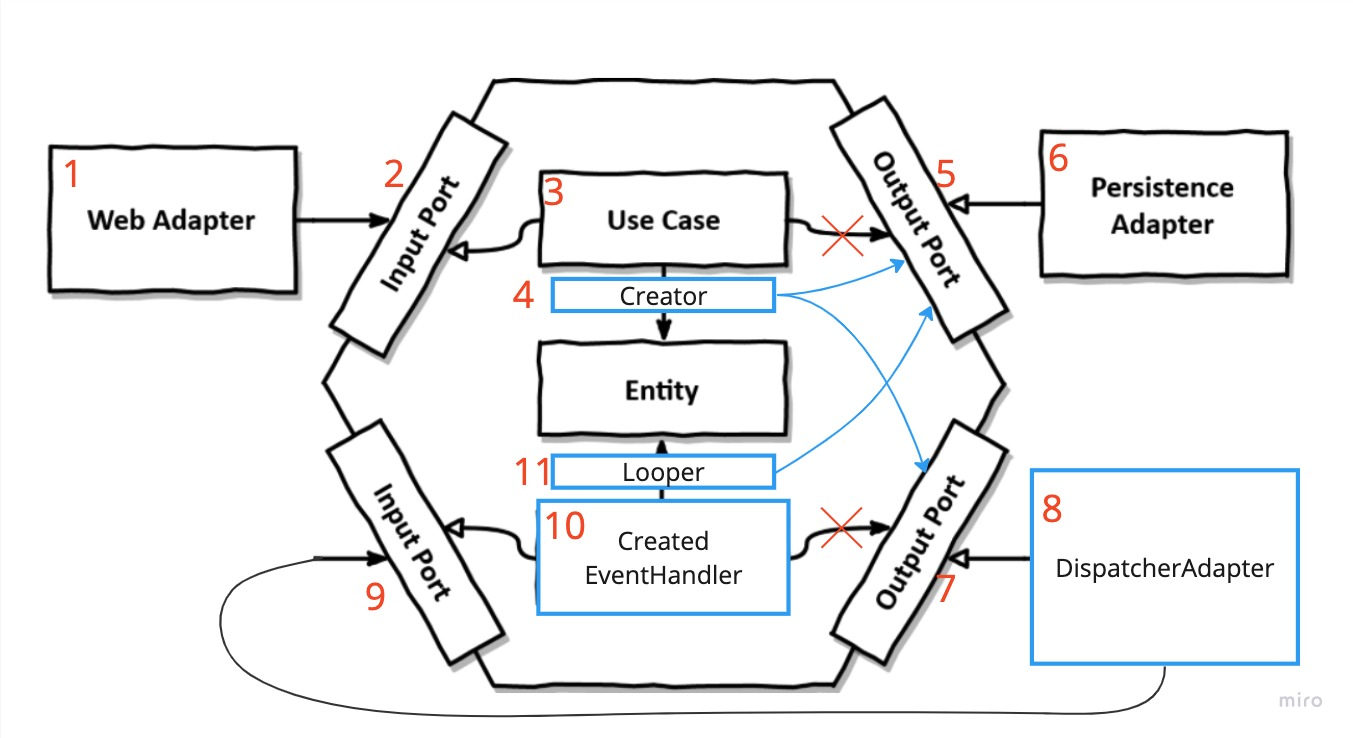
\includegraphics[height=0.3\textheight]{./part/Ejecucion/Seguimiento/CreateTaskUseCase/img/CreateTaskHexagonalDiagram}
    \caption{Hexagonal architecture diagram}\label{fig:CreateTaskHexagonalDiagram}
\end{figure}

\begin{figure}[H]
    \centering
    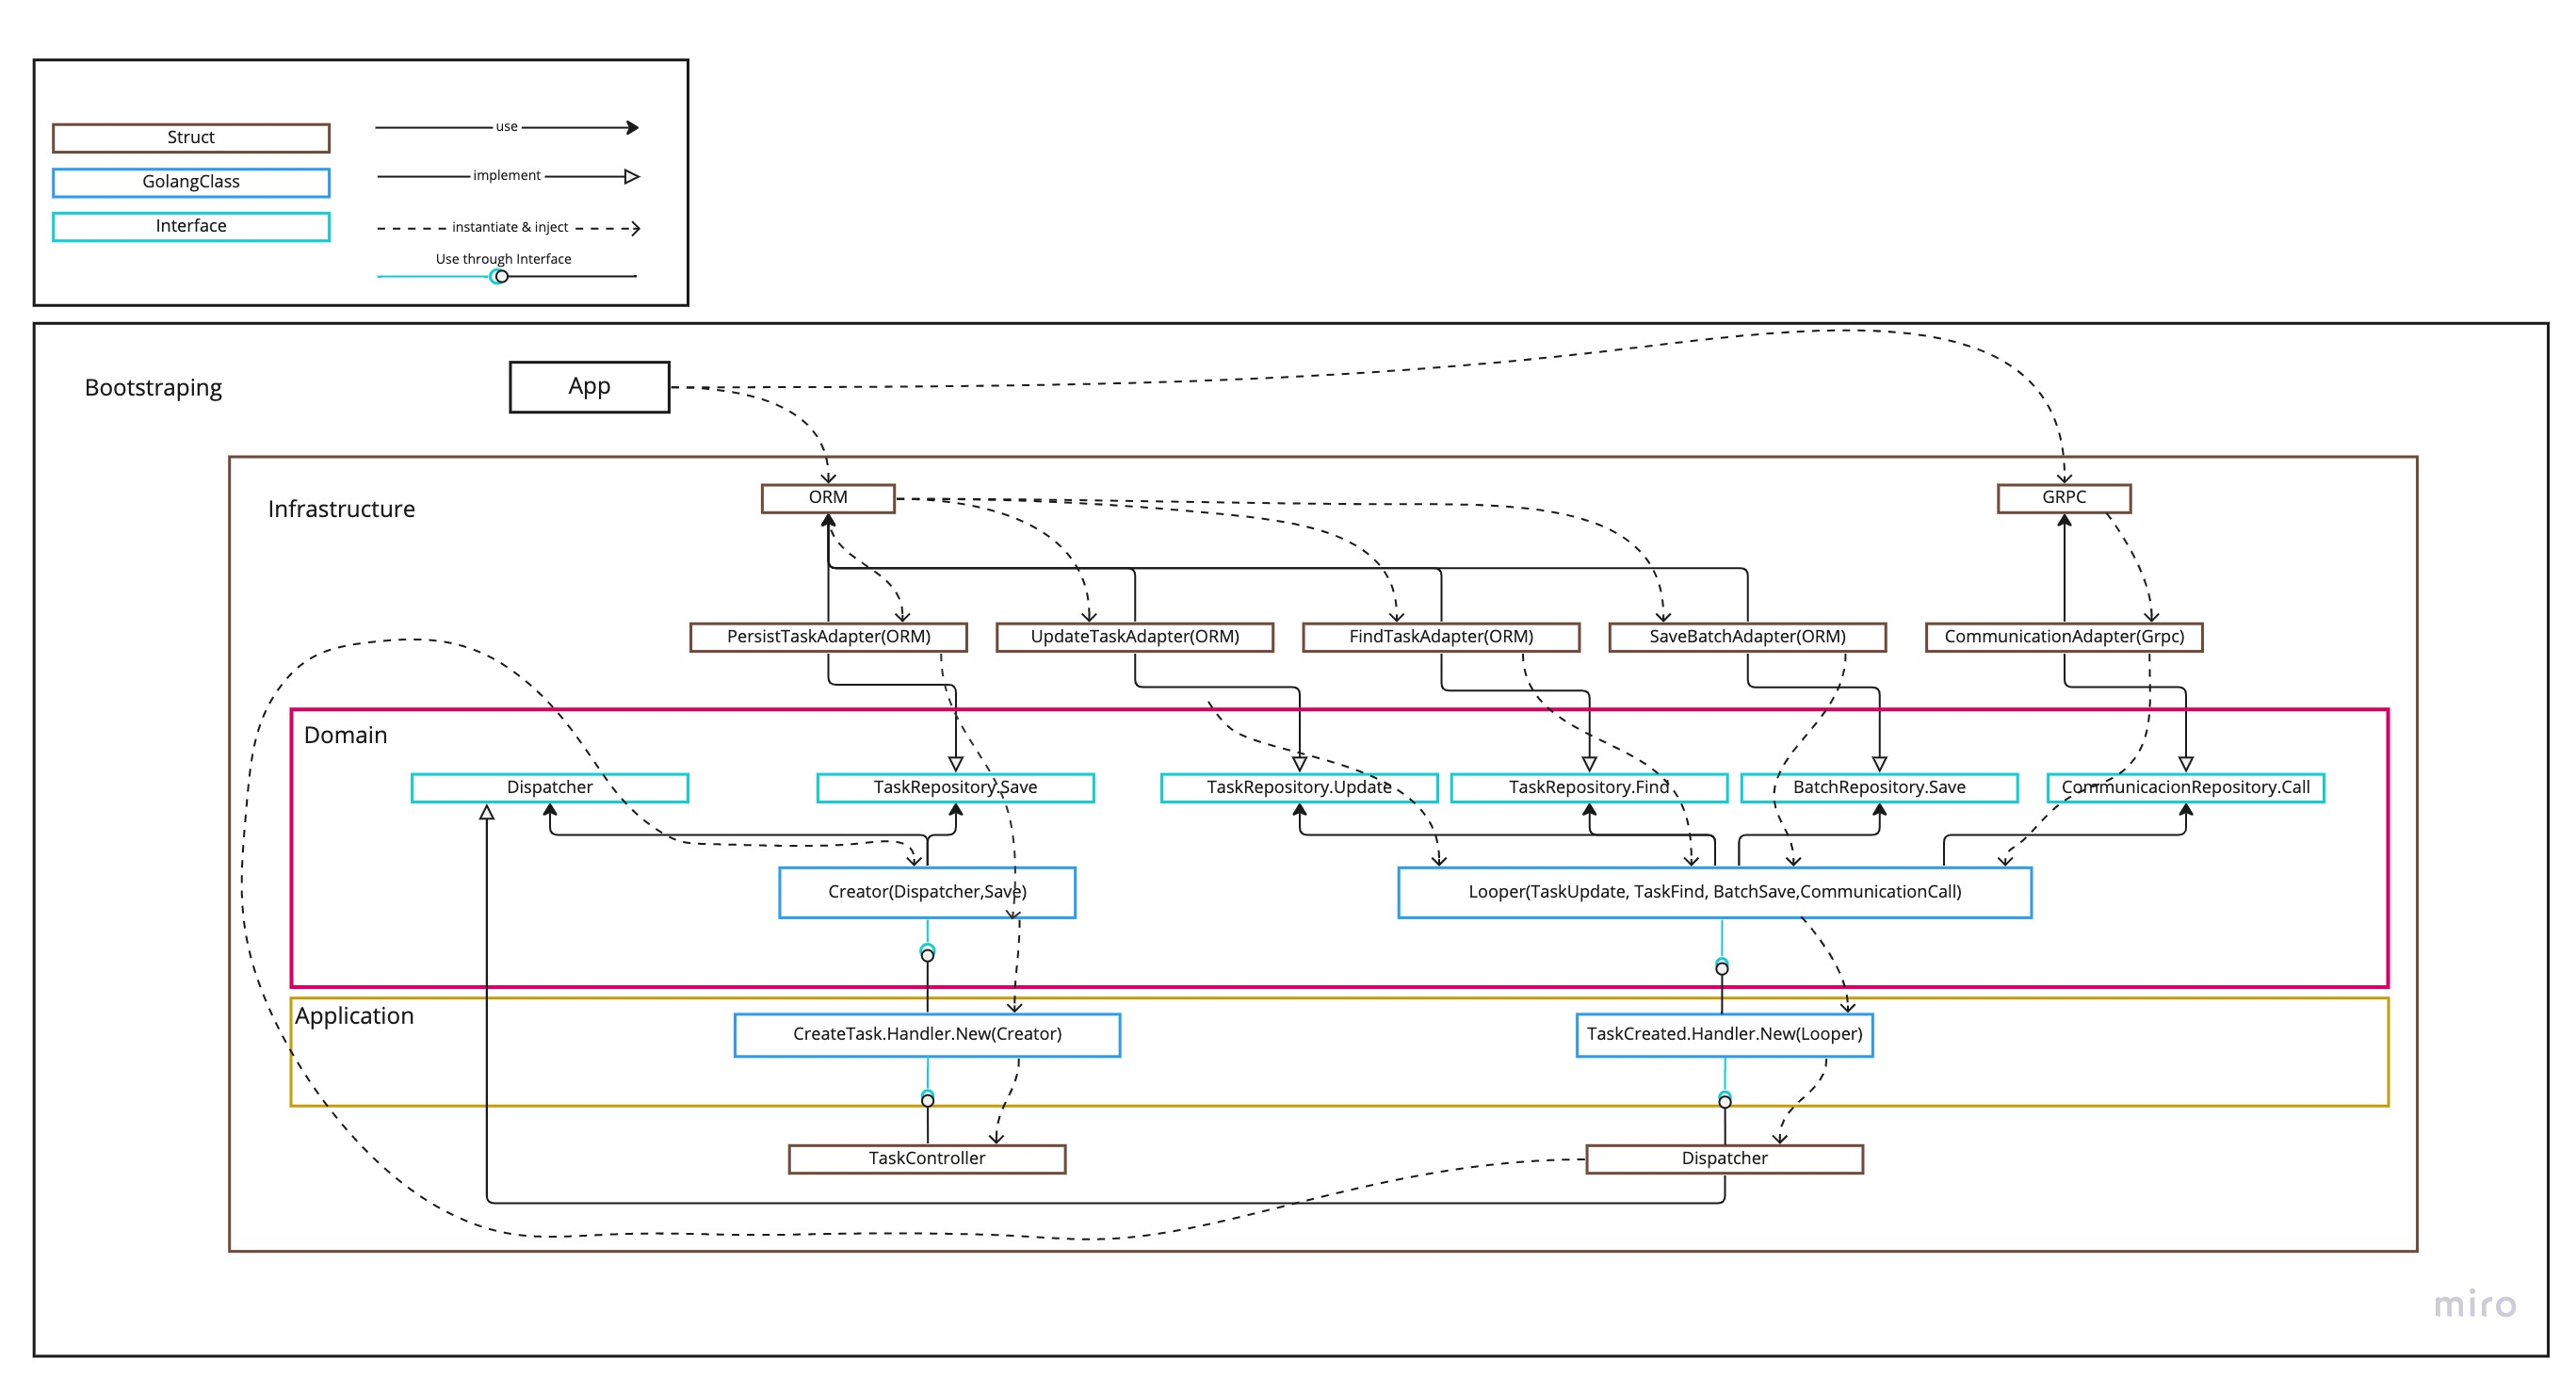
\includegraphics[height=0.3\textheight]{./part/Ejecucion/Seguimiento/CreateTaskUseCase/img/createTaskUseCaseArchitecture}
    \caption{CreateTaskUseCase hexagonal architecture diagram}\label{fig:createTaskUseCaseArchitecture}
\end{figure}

Acercandonos más al código podemos ver en el diagrama \ref{fig:createTaskUseCaseArchitectureFolderStructure} cómo es el uso entre los componentes que exísten en la estructrura de carpetas.

\begin{figure}[H]
    \centering
    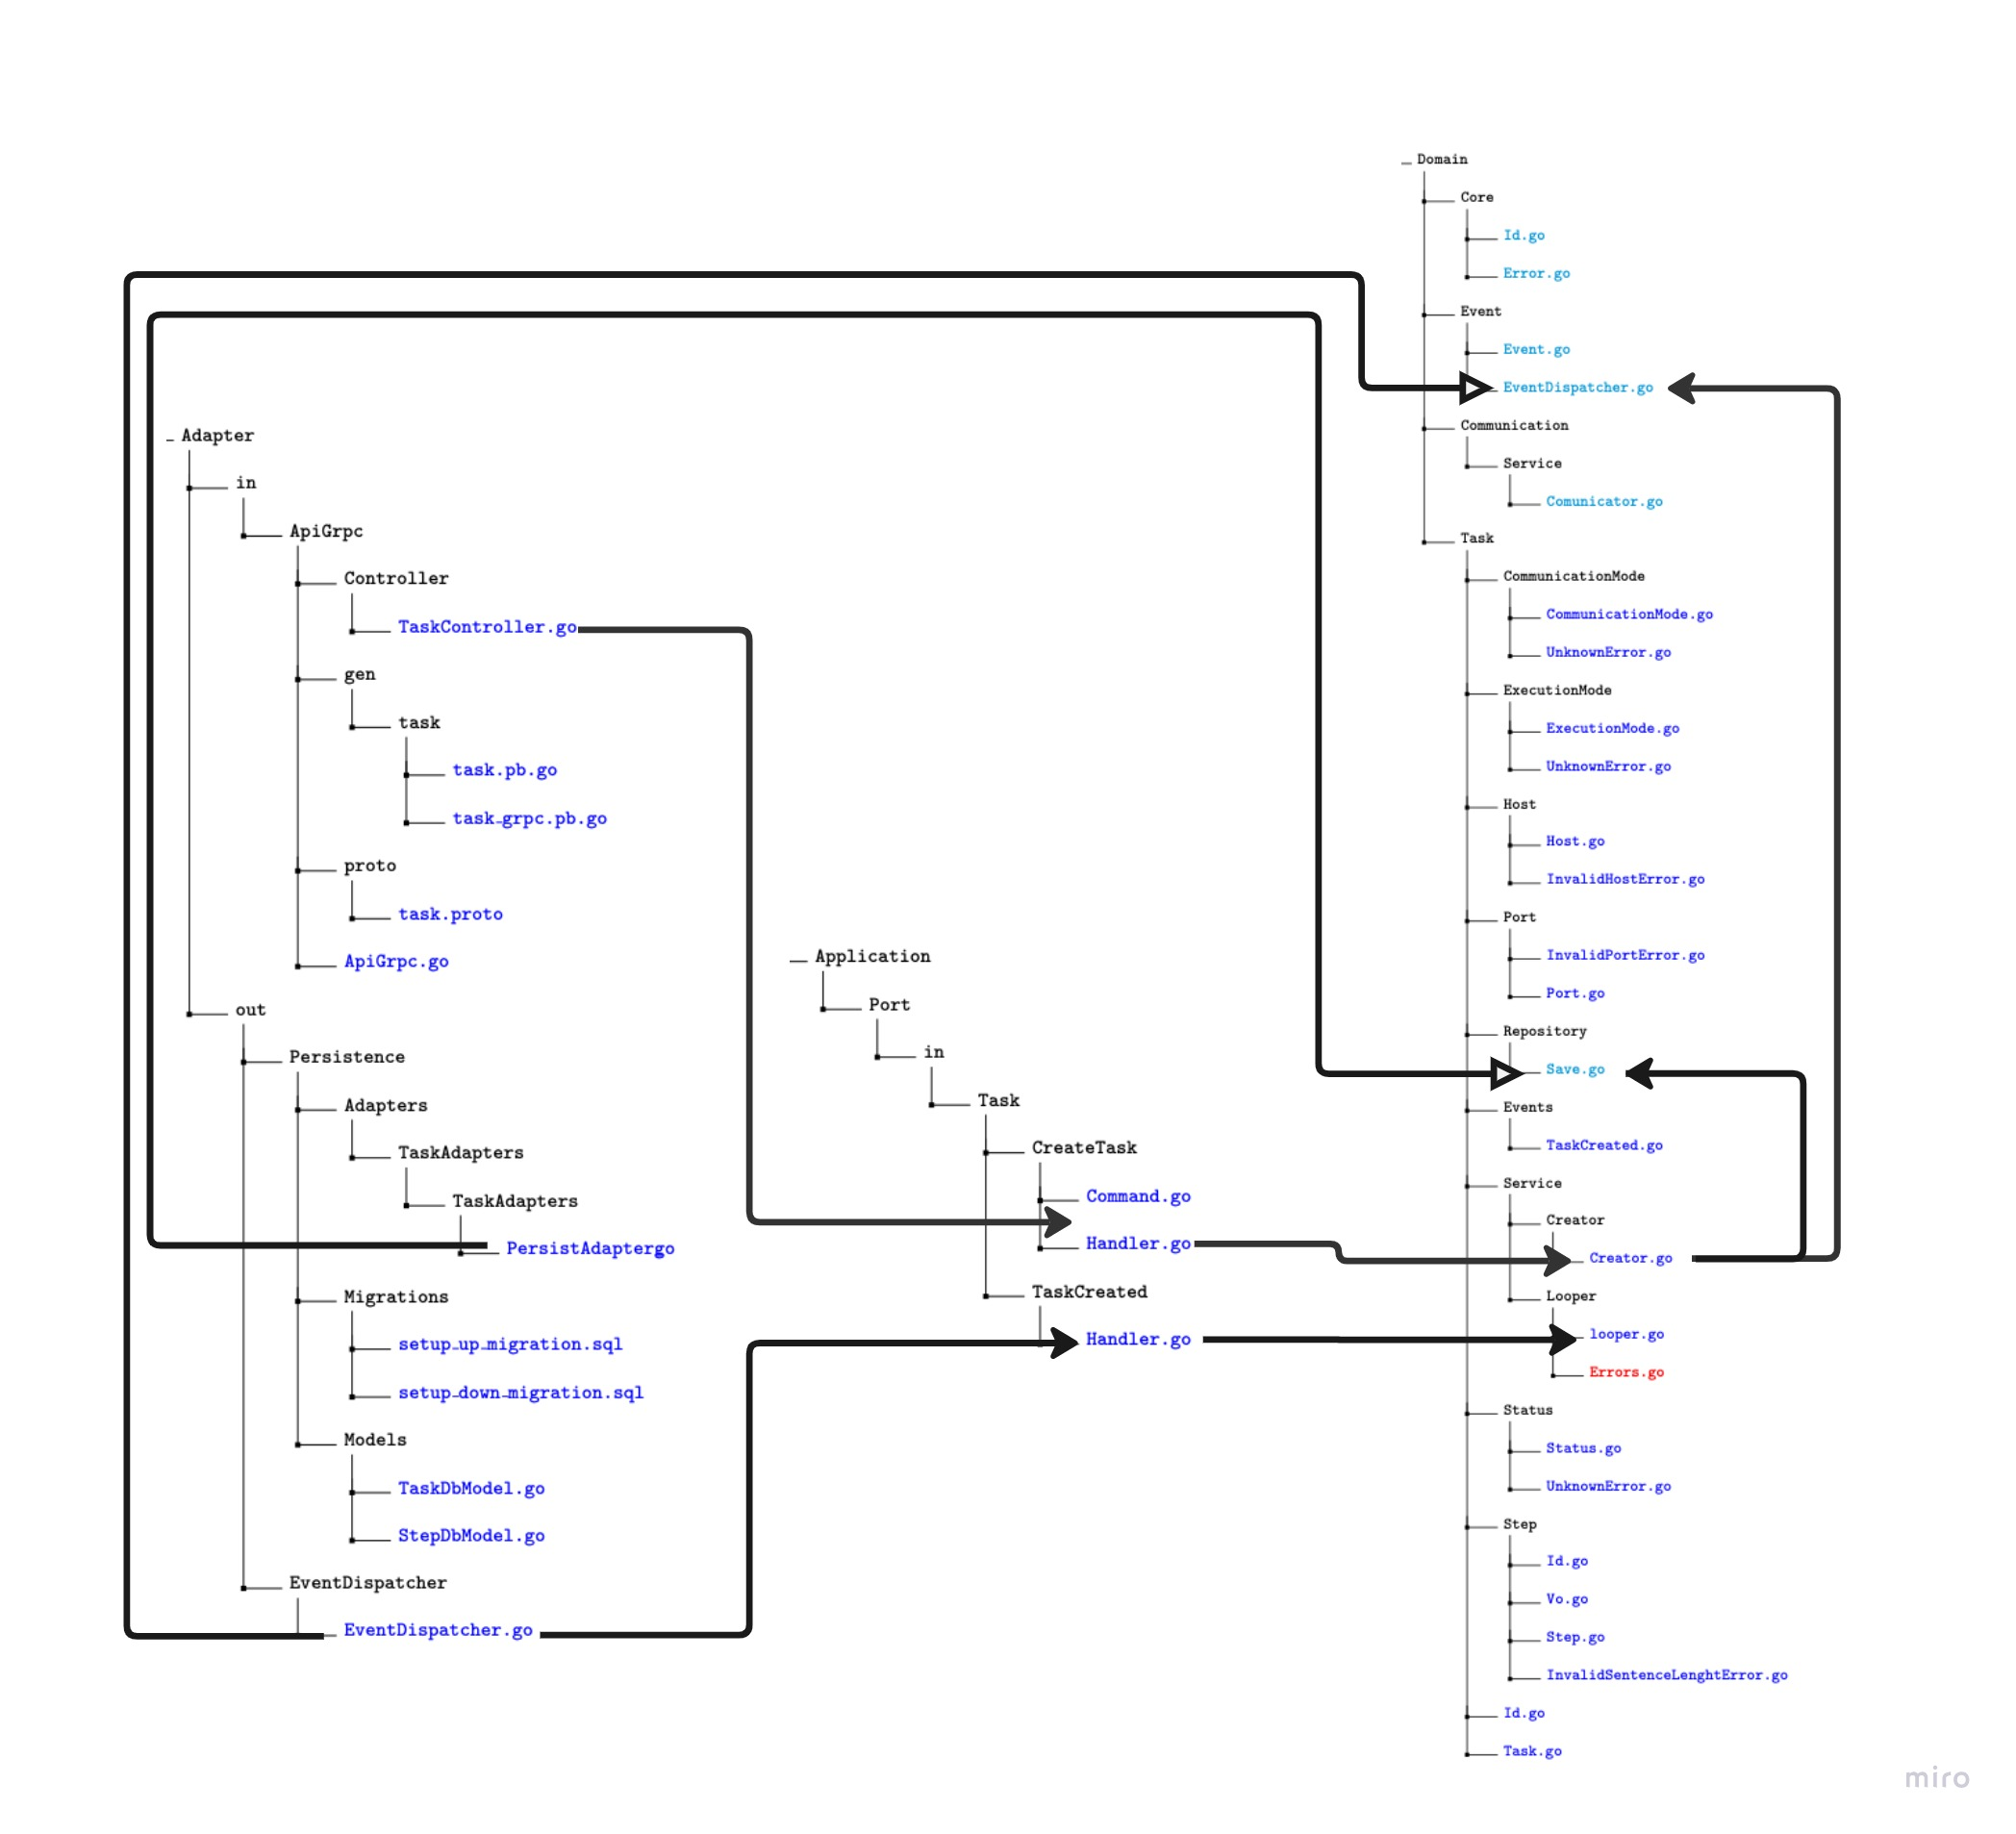
\includegraphics[height=0.5\textheight]{./part/Ejecucion/Seguimiento/CreateTaskUseCase/img/PFM - CreateUseCaseFolderStructure}
    \caption{CreateTaskUseCase folder Structure}\label{fig:createTaskUseCaseArchitectureFolderStructure}
\end{figure}

%Un punto interesante a comentar es el concepto de la estrategia de mapping que hay entre capas. Cada capa requiere sus objetos de trabajo. Tal y como sale descrito en \cite{TomHombergs2019GYHD} Tenemos tantas estratégias como atajos dentro de este paradigma queramos asumir. podemos ver en la figura \ref{fig:mapping types} Los tipos de mapping que se documentan en este libro:
%\begin{itemize}
%    \item The NoMapping Strategy
%    \item The Two-Way MappingStrategy
%    \item The Full MappingStrategy
%    \item The One-Way MappingStrategy
%\end{itemize}

Con respecto a la estrategia de mapping Golang nos permite hacer un full strategy casi por defecto porque al necesitar la implementaci'on de clase para garantizar la cohesión ya estamos utilizando interfaces para todas las clases. Así que en este caso utilizamos un fullMapping adaptado. lo cierto es que las versiones intermedias son todas las combinaciones posibles.

De cara a decidir extraemos la recomendacion de  \cite{TomHombergs2019GYHD}:"
we might start with a simple strategy that allows us to quickly evolve the code and later move to a more complex one that helps us to better decouple the layers.
In order to decide which strategy to use when, we need to agree upon a set of guidelines within the team. These guidelines should answer the question which mapping strategy should be the first choice in which situation. They should also answer why they are first choice so that we’re able to evaluate if those reasons still apply after some time."

Al final se trata de tomar una decisión en equipo, documentar las razones y ser consistentes. Reevaluar las razones ante un reto que las ponga a prueba y tomar o no la decisión de cambiar la estrategia.

En nuestra opinión dentro de la estrategia fullmapping se debe implementar un modelo tanto de entrada, como ya se contempla, como de salída. Es decir, la respuesta que hay entre cada capa también debe ser mappeada, podemos ver el patrón readptado en la figura \ref{fig:GetHandMapping}

\begin{figure}[H]
    \centering
    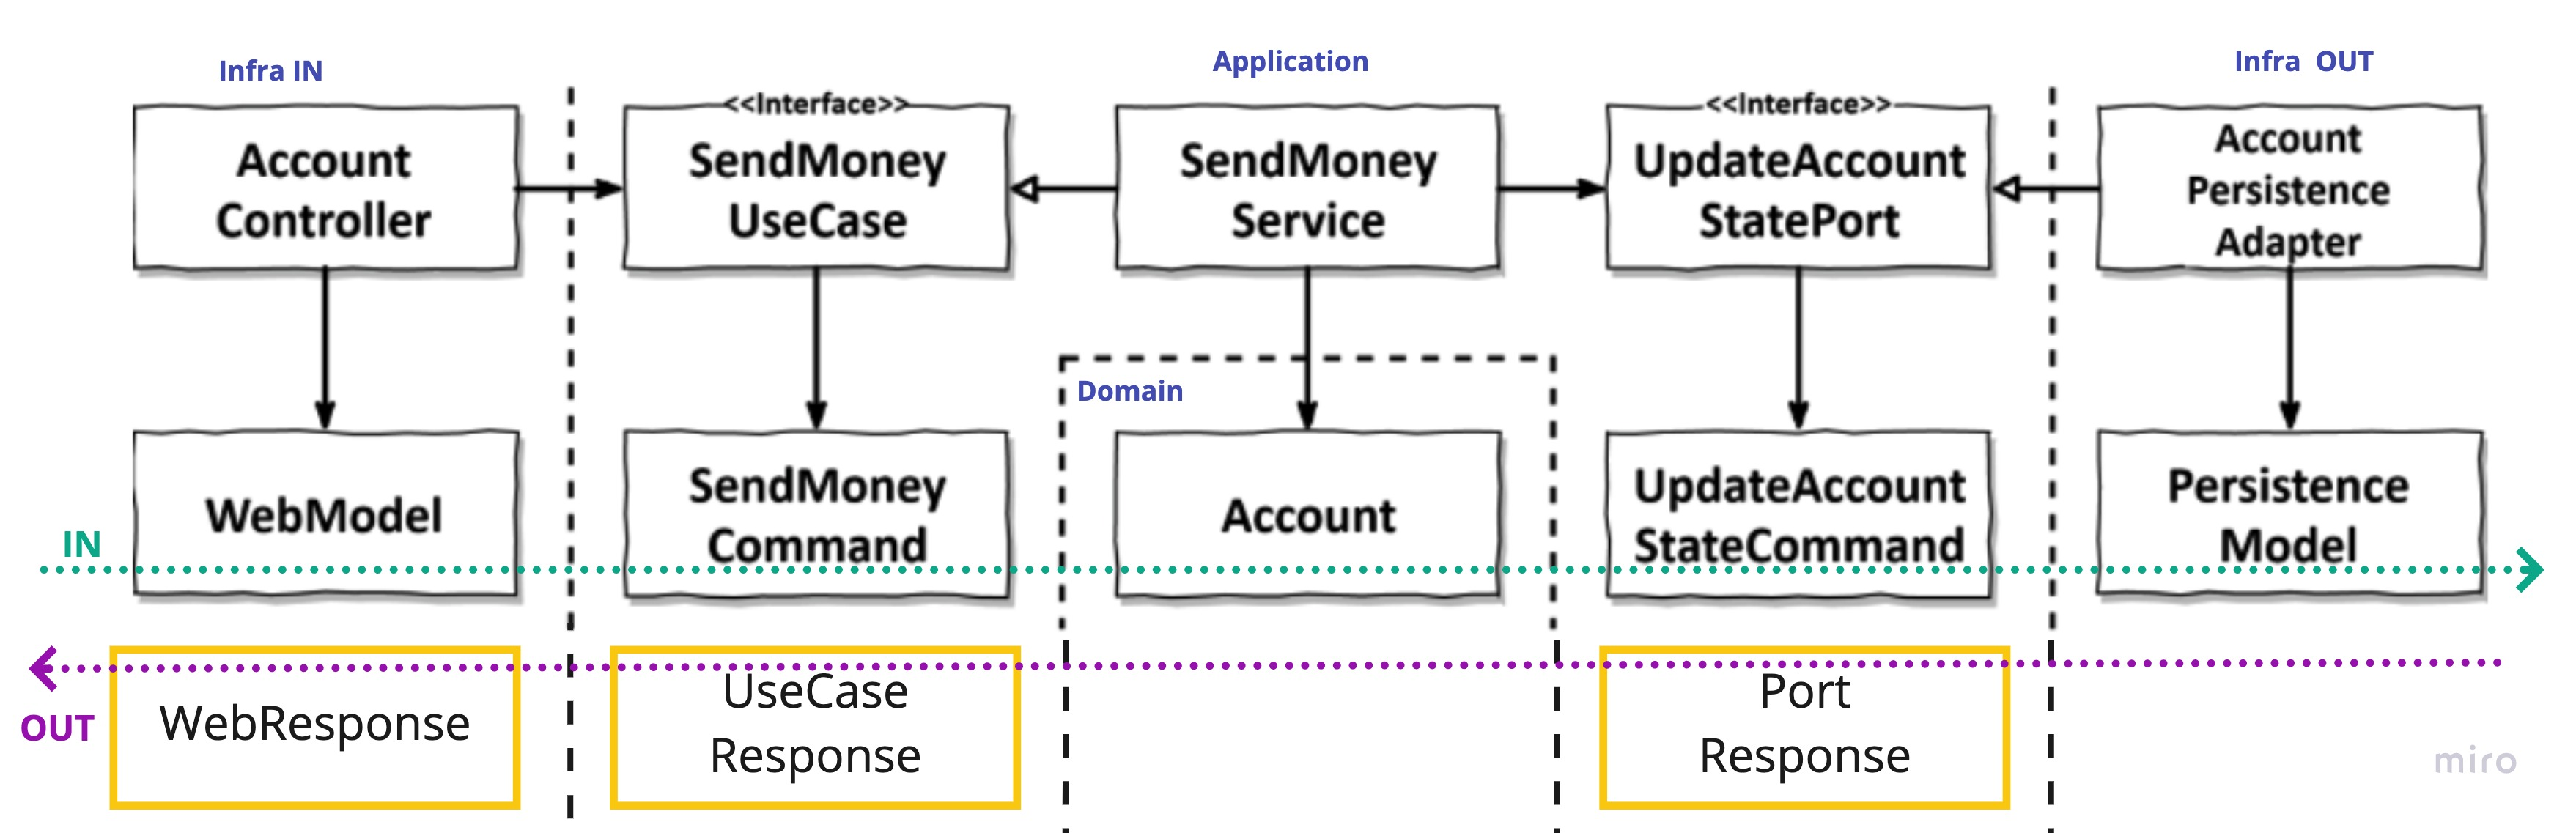
\includegraphics[height=0.2\textheight]{./part/Ejecucion/Seguimiento/CreateTaskUseCase/img/PFM - GetHandMapping}
    \caption{CreateTaskUseCase folder Structure\cite{TomHombergs2019GYHD}}\label{fig:GetHandMapping}
\end{figure}

Claramente esto aumenta la burocracia y finalmente la opción que hemos tomado se puede ver en la figura\ref{fig:CreateTaskUseCaseMapping}

En rojo se han marcado los atajos que se han tomado, es decir, el mapeo que no se ha implementado. El objetivo es aislarse bien de los puertos de entrada, es decir el GRPC, y no tanto de los puertos de salida. ya que la persistencia está bien aislada mediante las interfaces. Dentro de los adaptadores se hará el trabajo de mappeo entre las entidades de dominio y los modelos de persistencia y se traducirá de nuevo a dominio para responder.

\begin{figure}[H]
    \centering
    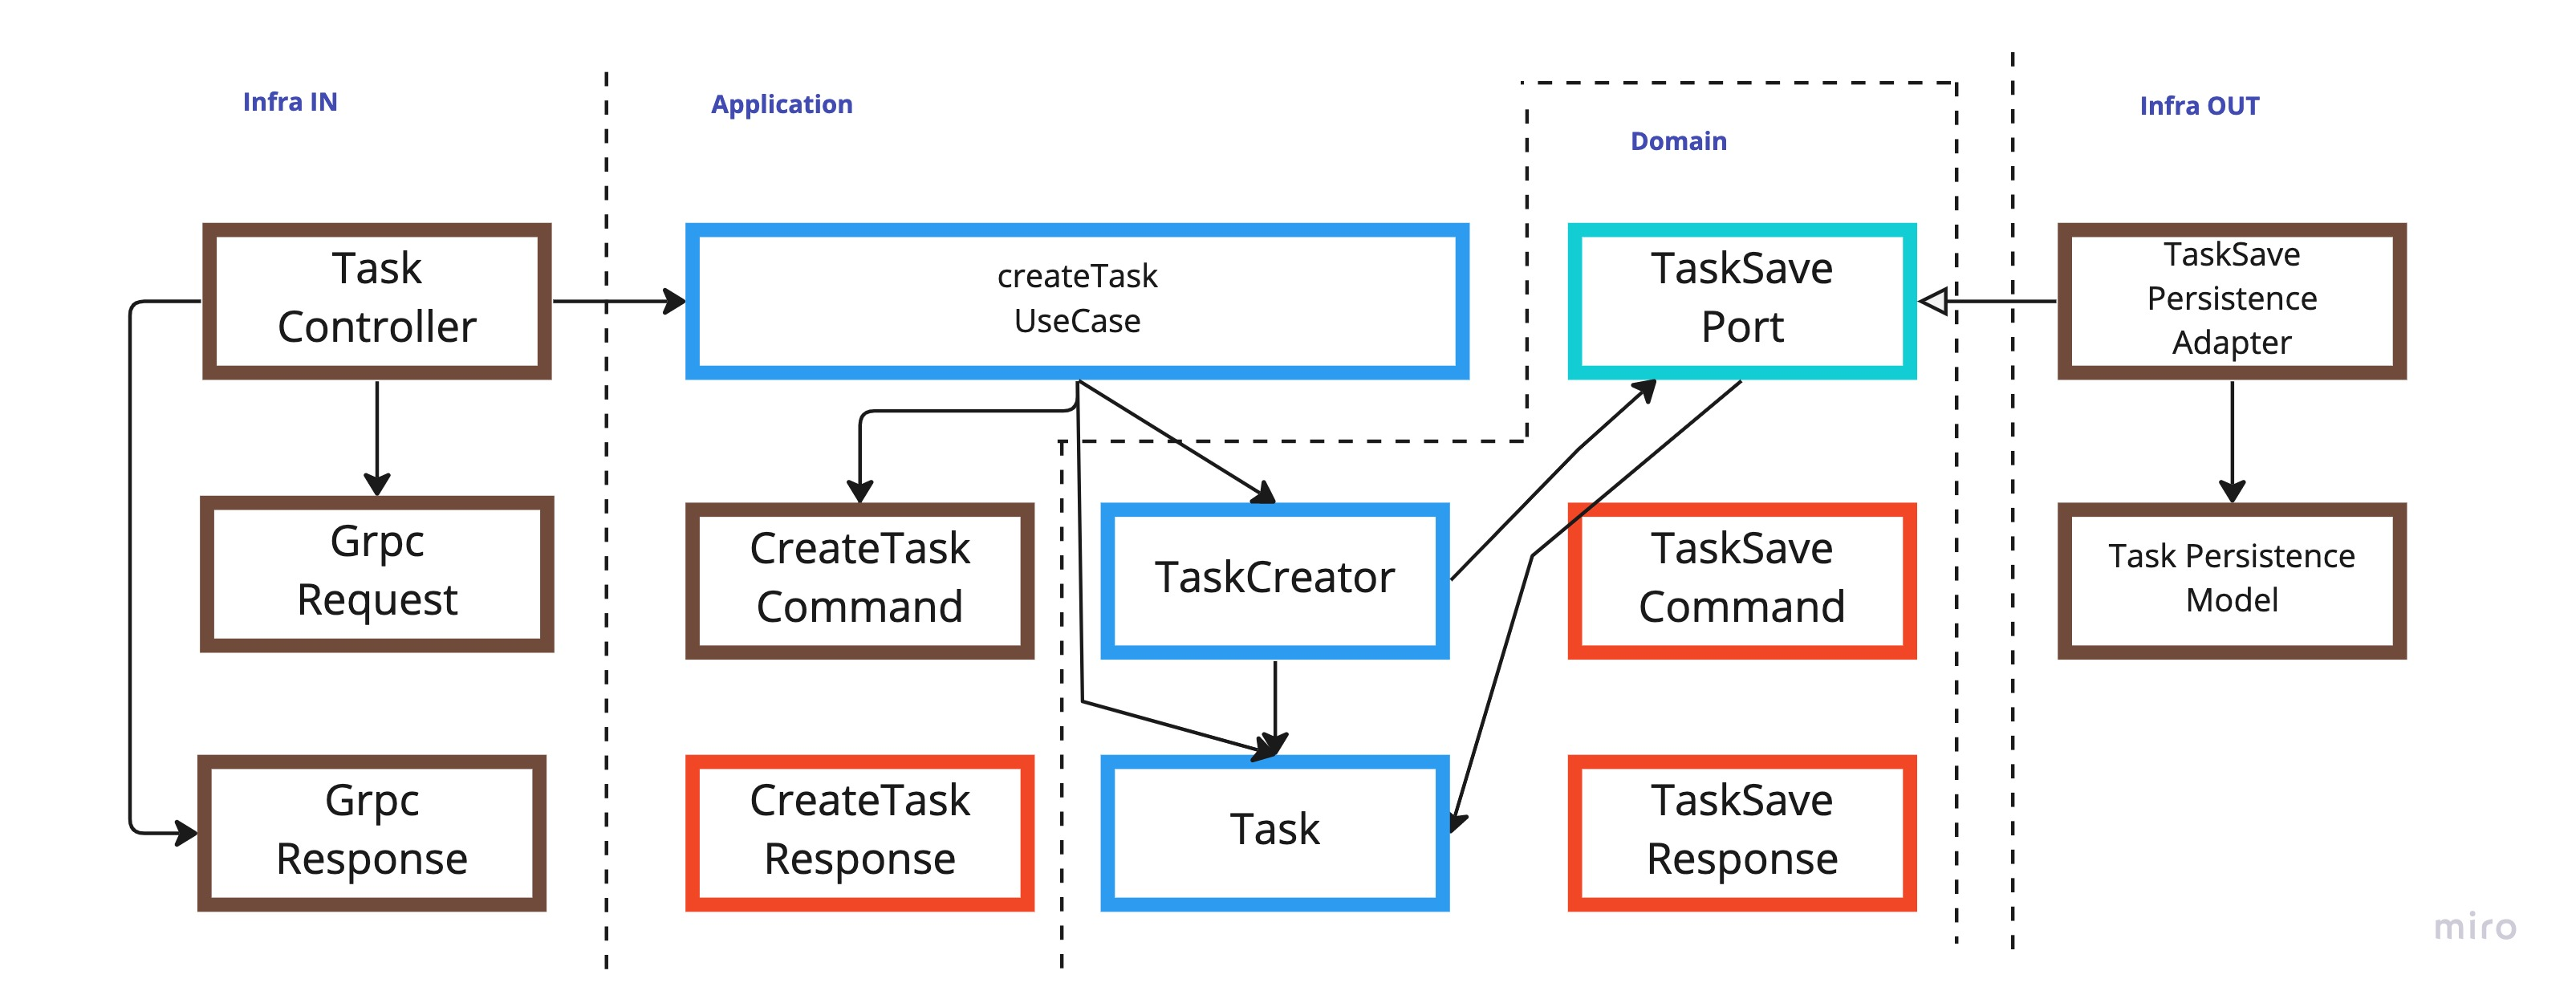
\includegraphics[height=0.2\textheight]{./part/Ejecucion/Seguimiento/CreateTaskUseCase/img/PFM - FinalMapping}
    \caption{CreateTaskUseCase folder Structure}\label{fig:CreateTaskUseCaseMapping}
\end{figure}

Ahora vamos a exponer el código final de este caso de uso, vamos a hacer referencia a:
\begin{itemize}
    \item TaskController \ref{fig:TaskControler}
    \item CreateTaskUseCase \ref{fig:CreateTaskUseCaseCode}
    \item Creator \ref{fig:Creator}
    \item SavePort \ref{fig:SavePort}
    \item PersistAdapter \ref{fig:SaveAdapter}
    \item DispatcherPort \ref{fig:DispatcherPort}
\end{itemize}

\begin{figure}[H]
    \centering
    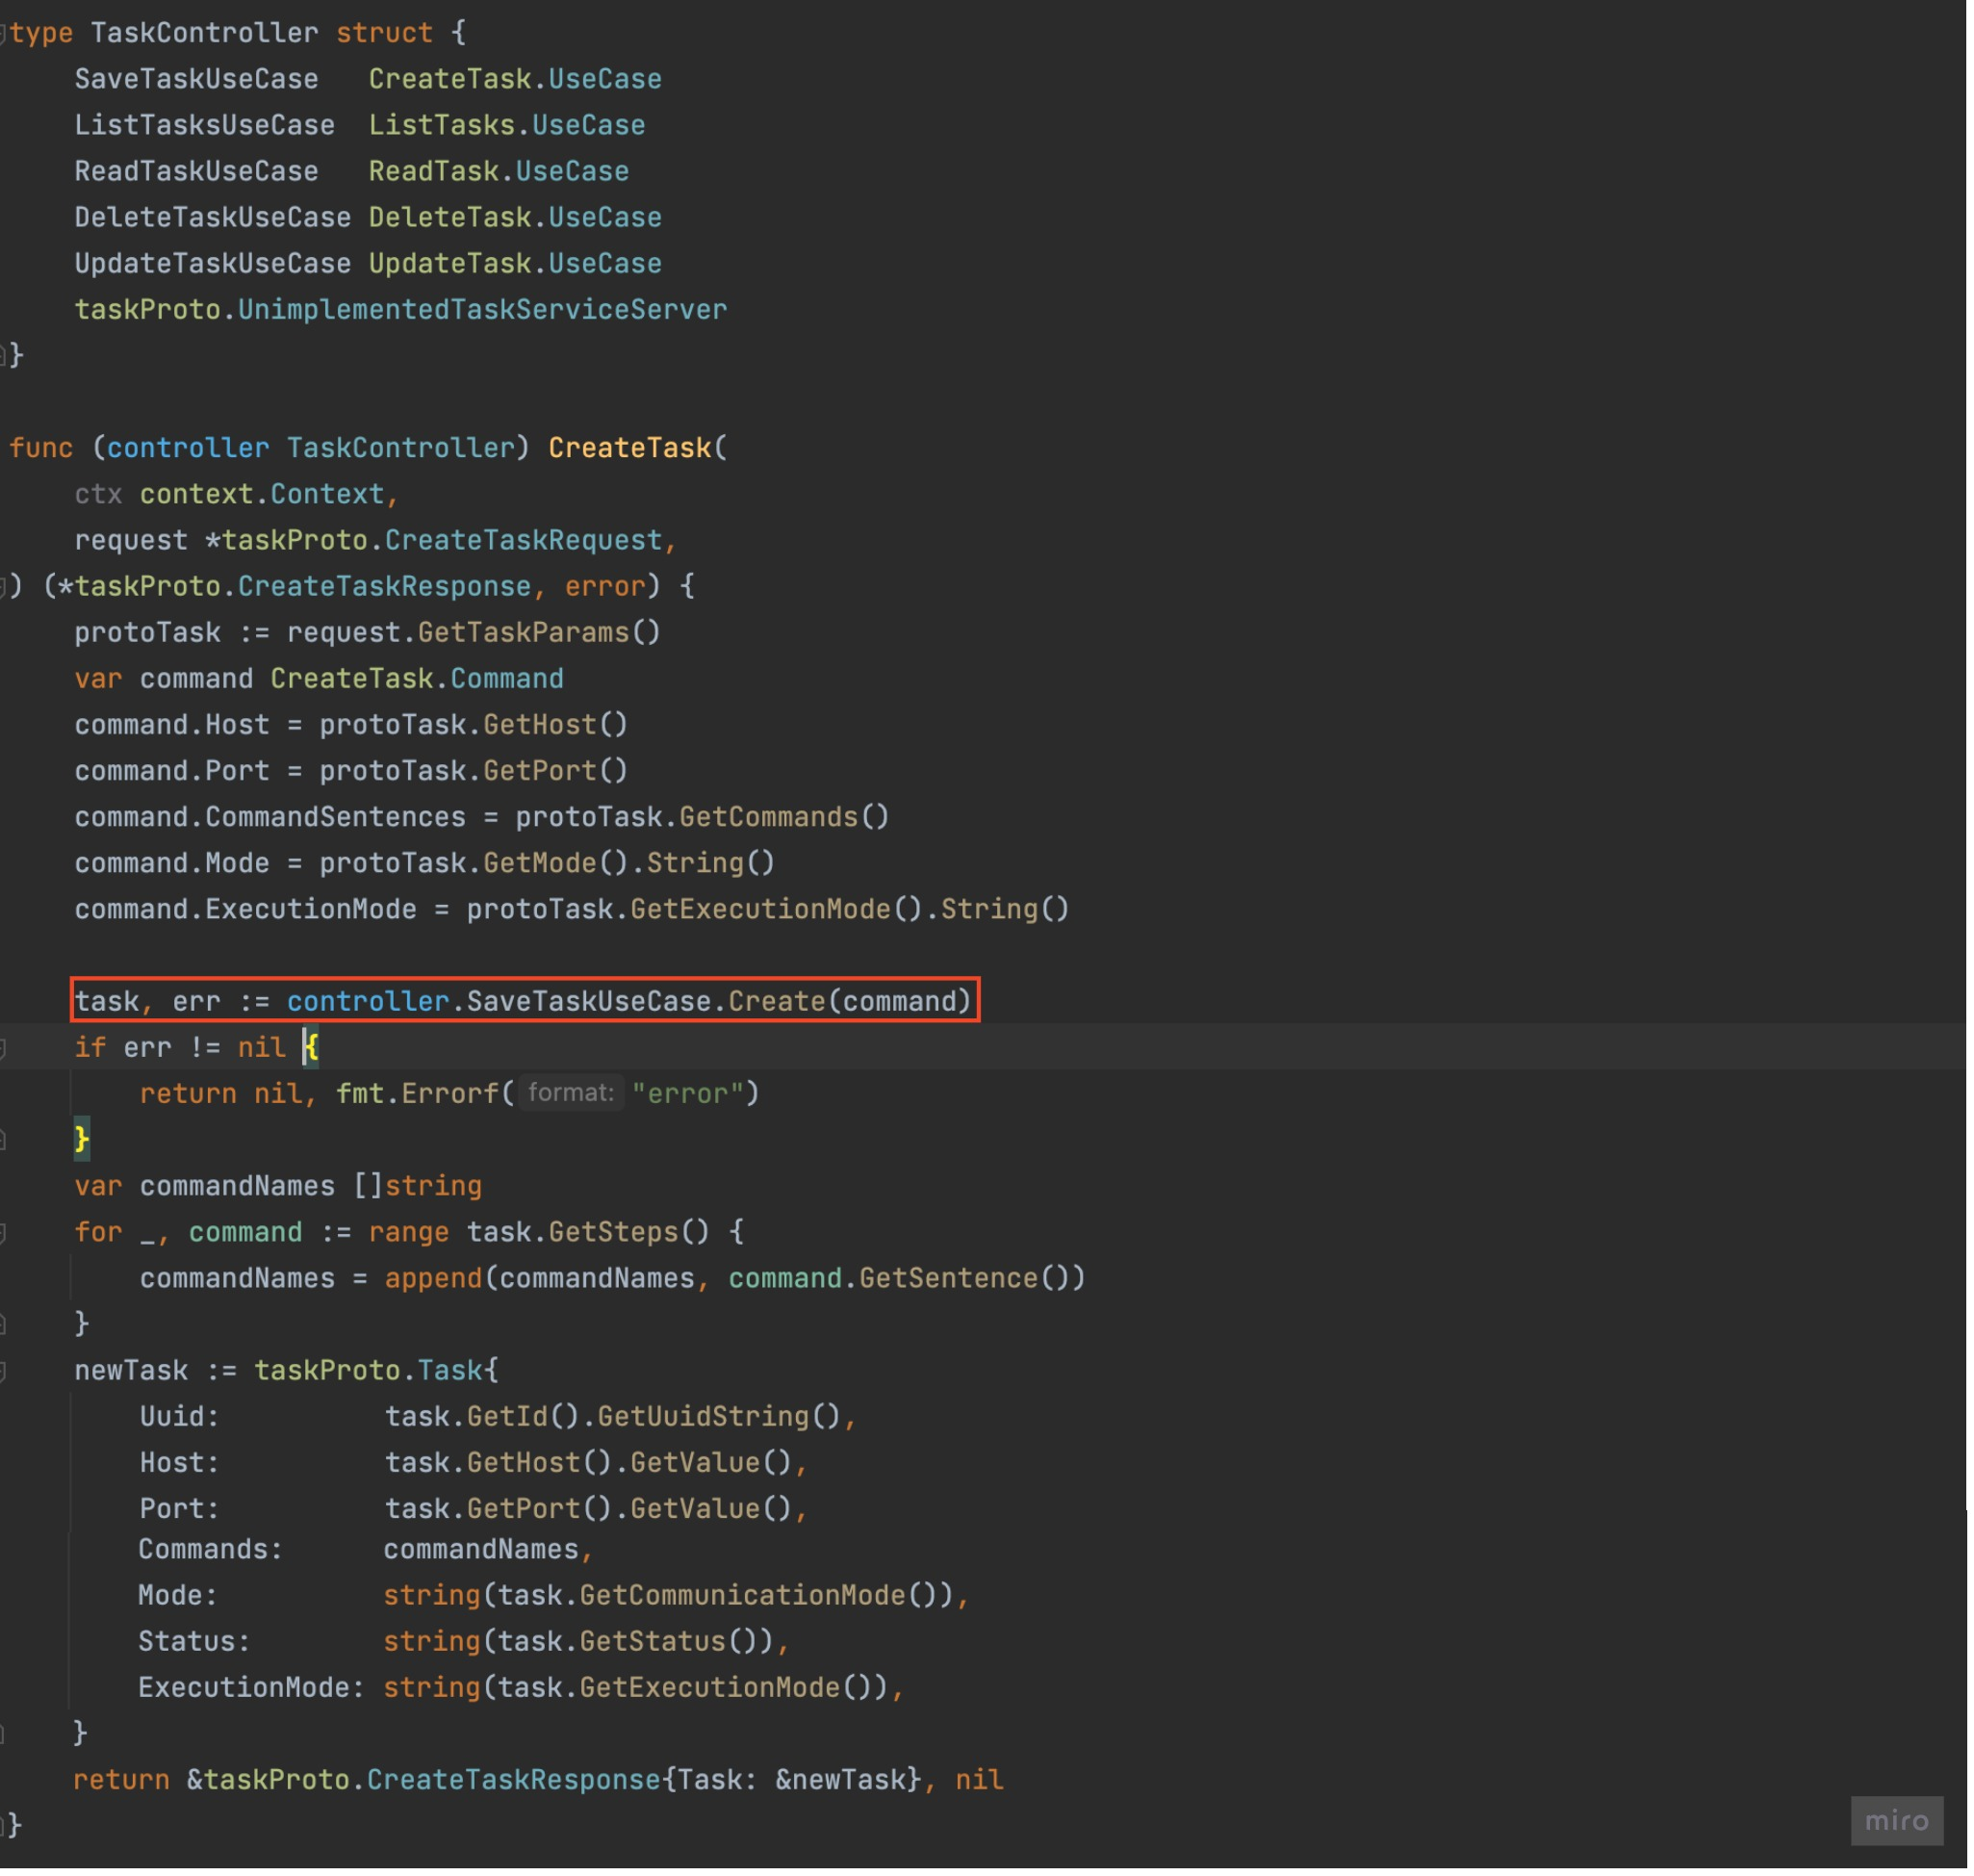
\includegraphics[height=0.5\textheight]{./part/Ejecucion/Seguimiento/CreateTaskUseCase/img/PFM - TaskController}
    \caption{TaskController.go}\label{fig:TaskControler}
\end{figure}

\begin{figure}[H]
    \centering
    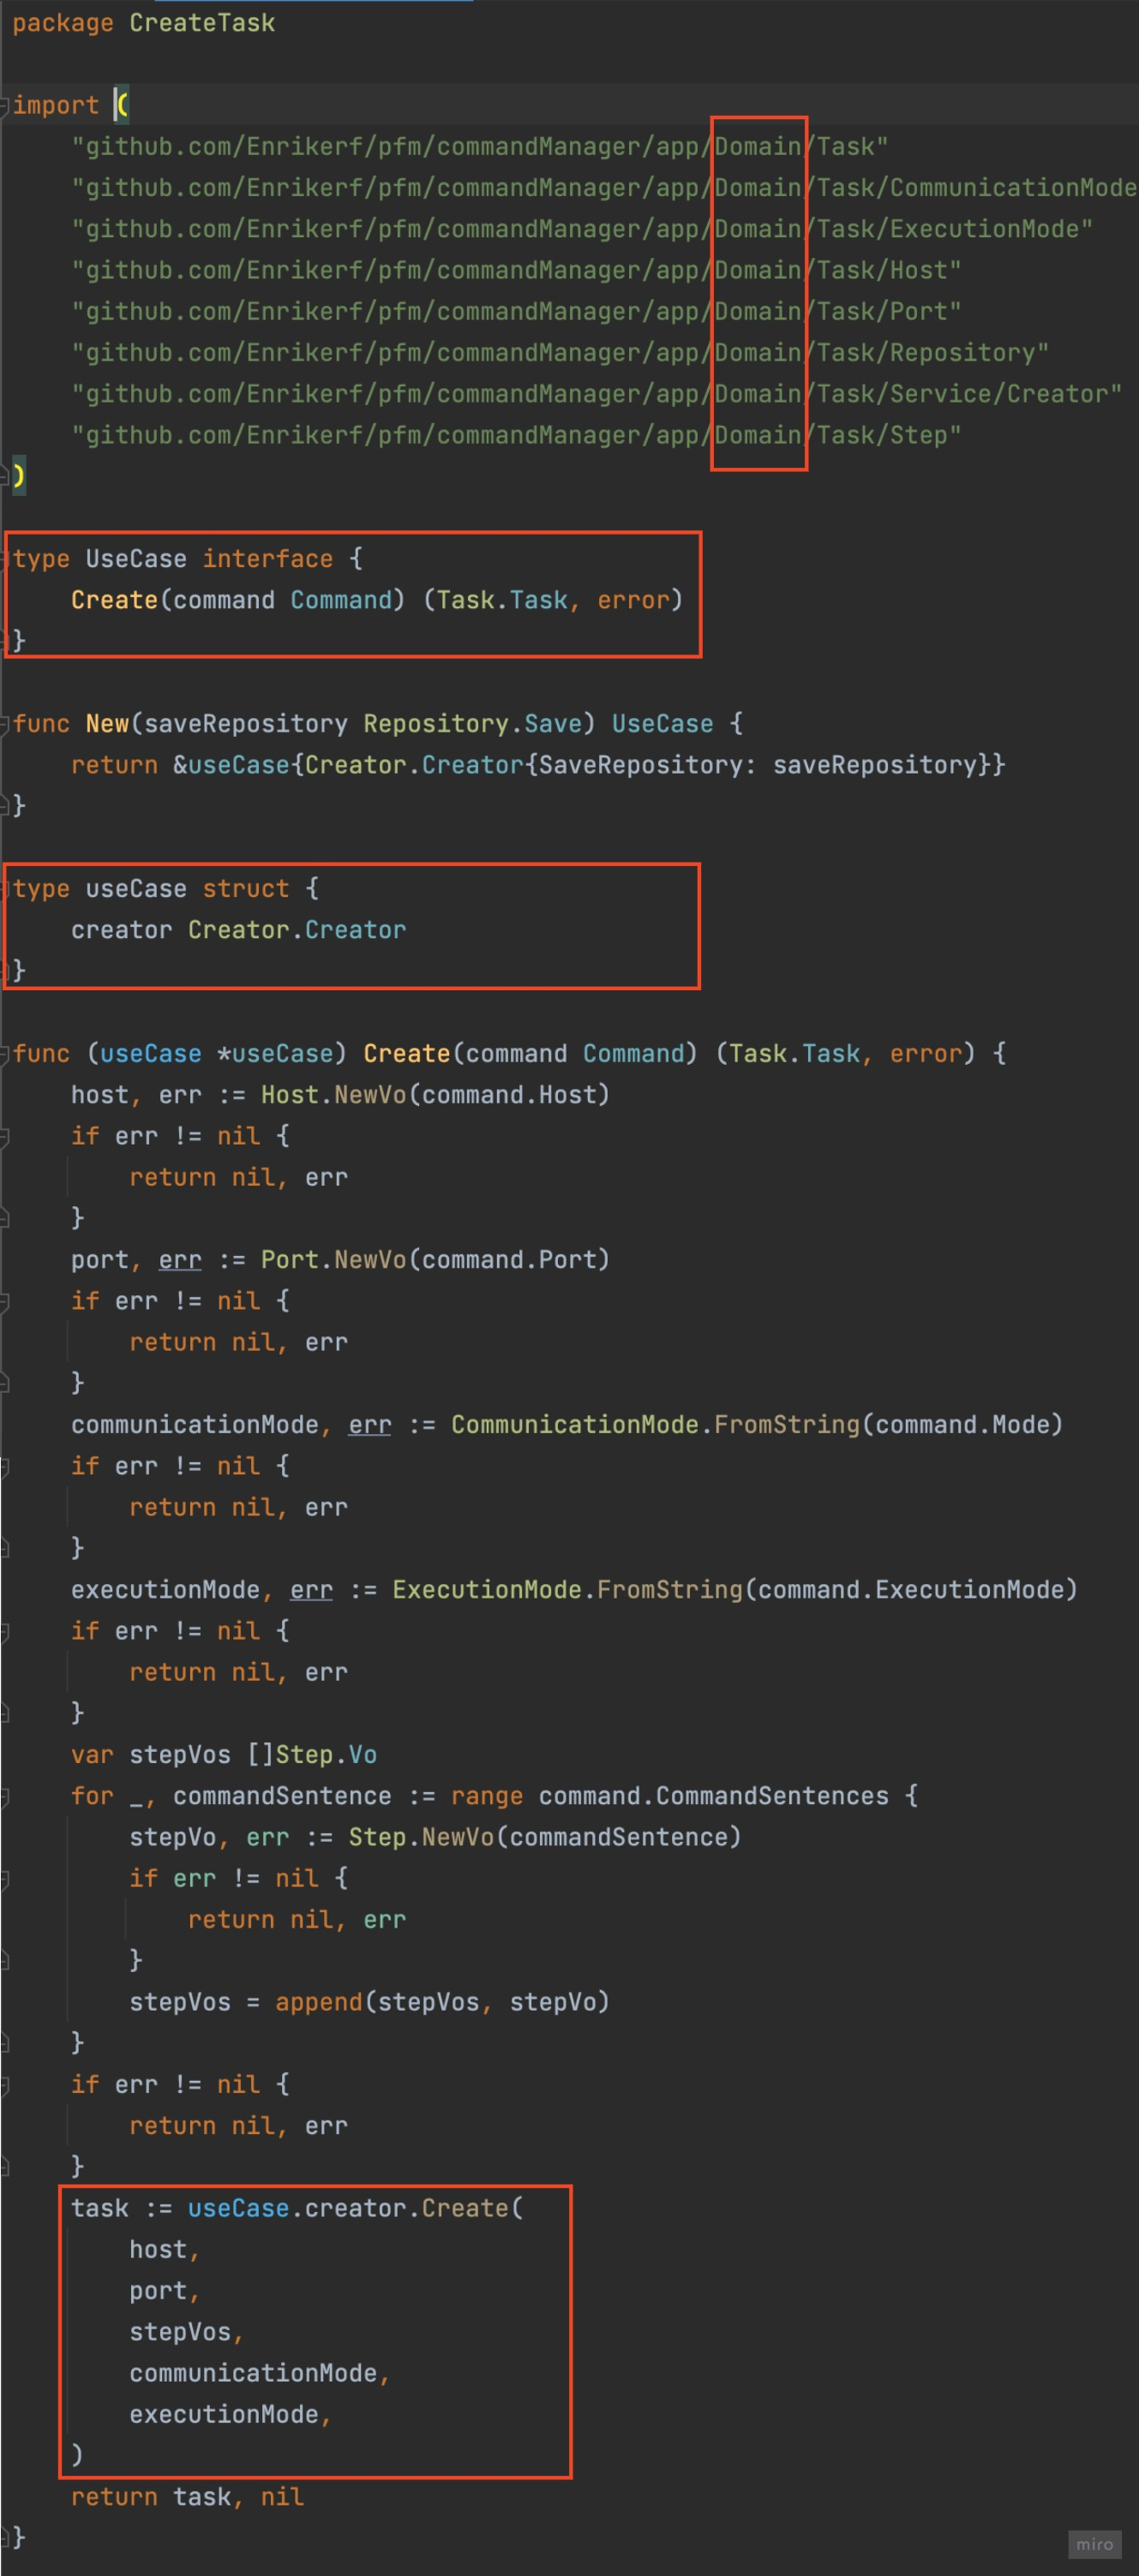
\includegraphics[height=0.5\textheight]{./part/Ejecucion/Seguimiento/CreateTaskUseCase/img/PFM - CreateTaskUseCaseCode}
    \caption{CreateTaskUseCaseCode.go}\label{fig:CreateTaskUseCaseCode}
\end{figure}

\begin{figure}[H]
    \centering
    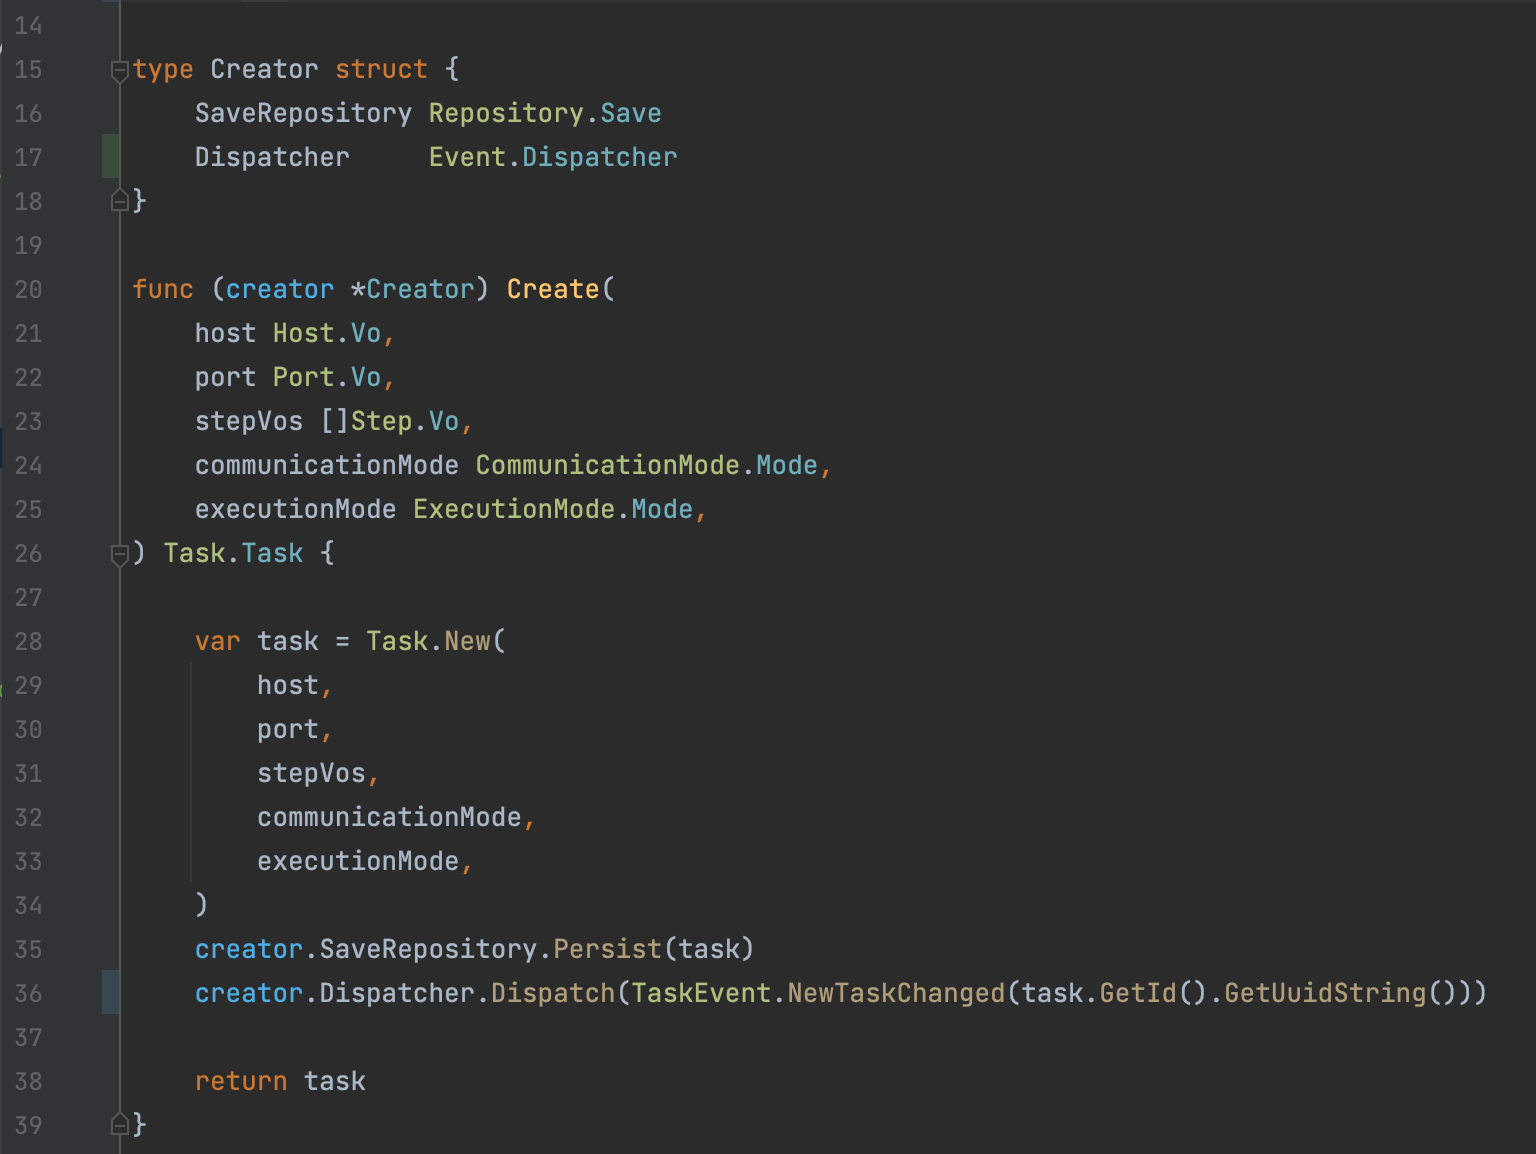
\includegraphics[height=0.5\textheight]{./part/Ejecucion/Seguimiento/CreateTaskUseCase/img/PFM - creator}
    \caption{Creator.go}\label{fig:Creator}
\end{figure}

\begin{figure}[H]
    \centering
    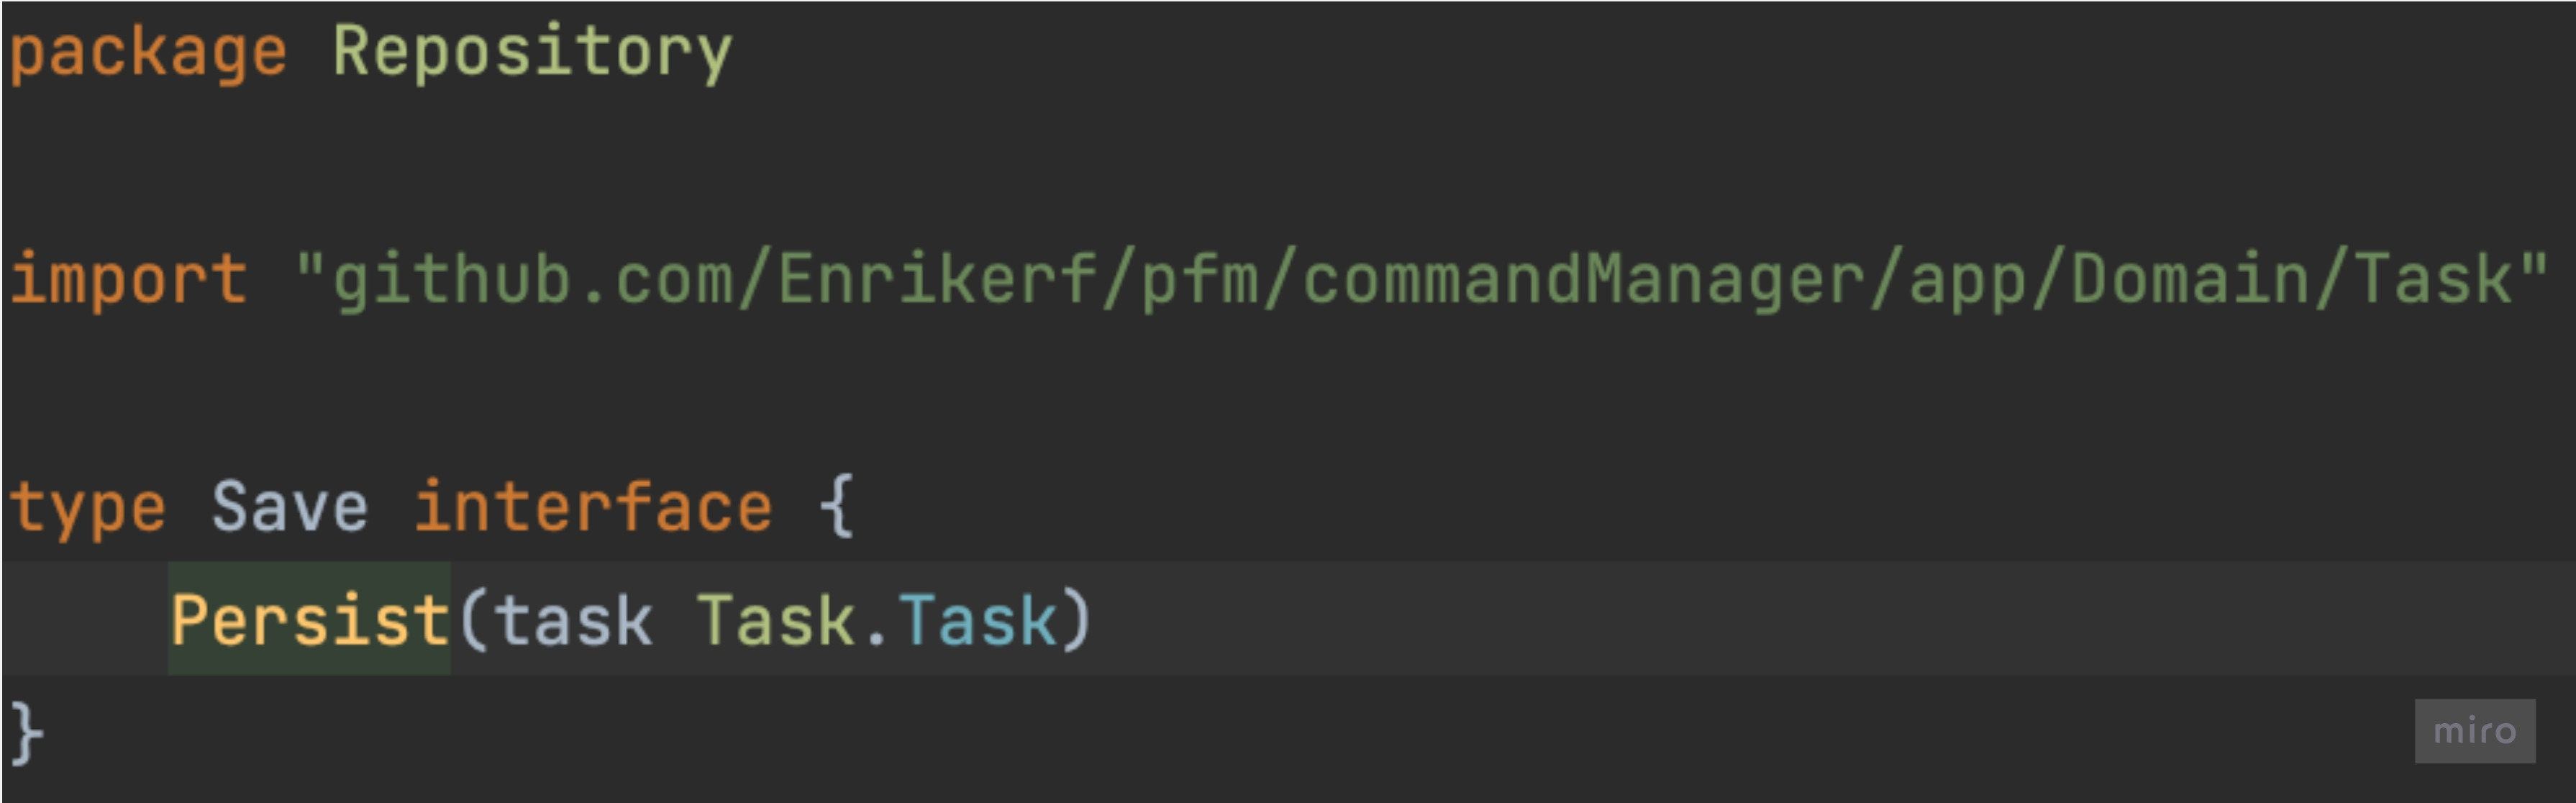
\includegraphics[height=0.2\textheight]{./part/Ejecucion/Seguimiento/CreateTaskUseCase/img/PFM - SavePort}
    \caption{Creator.go}\label{fig:SavePort}
\end{figure}

\begin{figure}[H]
    \centering
    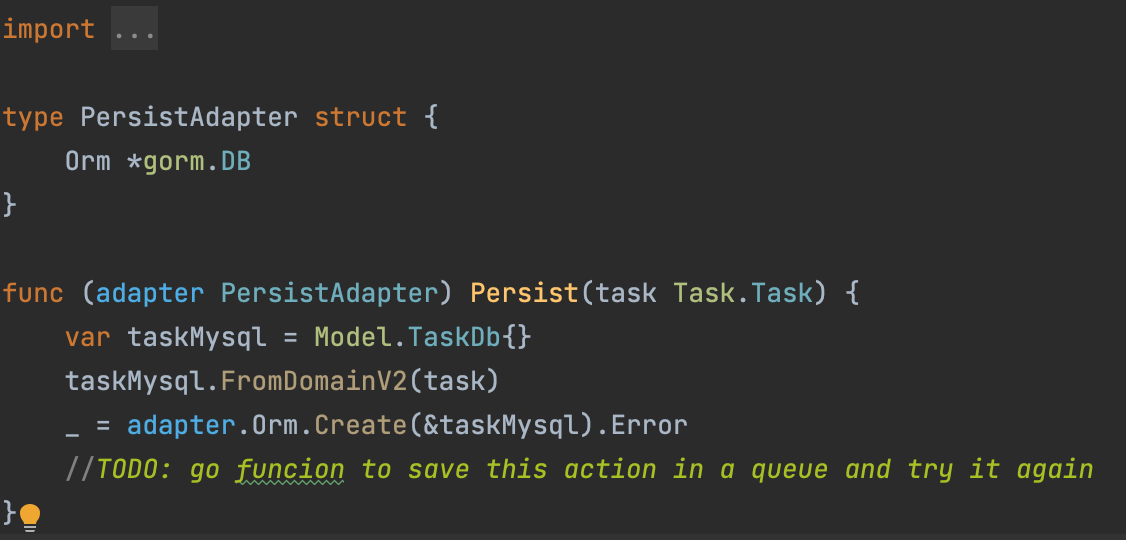
\includegraphics[height=0.2\textheight]{./part/Ejecucion/Seguimiento/CreateTaskUseCase/img/PFM - SaveAdapter}
    \caption{Creator.go}\label{fig:SaveAdapter}
\end{figure}

\begin{figure}[H]
    \centering
    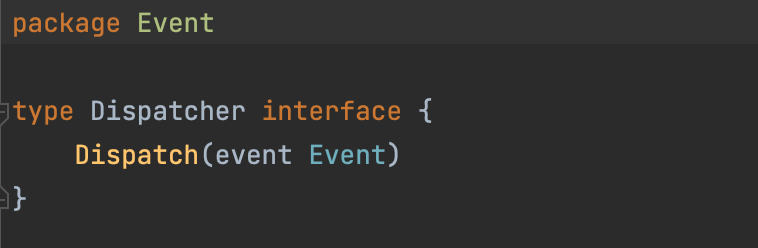
\includegraphics[height=0.2\textheight]{./part/Ejecucion/Seguimiento/CreateTaskUseCase/img/PFM - Dispatcher}
    \caption{Creator.go}\label{fig:DispatcherPort}
\end{figure}
\subsubsection{TaskLooper}
%    
El codigo de colores utilizado en los diagramas de esta seccion se refieren al equivalente a clase en golang en azul y a las interfaces puras en turquesa  y a los structs en marron

%El tipico diagráma cuando se habla de arquitectura hexagonal es tal y como se muestra en la figura\ref{fig:hexagonalDiagram} Si bien consideramos que no tiene mucho sentido y de cara a la parte didáctica confunde, ya que el hexágono es una simple licencia estética. en el caso de existir más puertos de salida y entrada que los representados el hexágono pierde todo el sentido y cuando se enfrenta por primera vez este diagrama se tiende a intentar descifrar el sentído del hexagono.
%
%\begin{figure}[H]
%    \centering
%    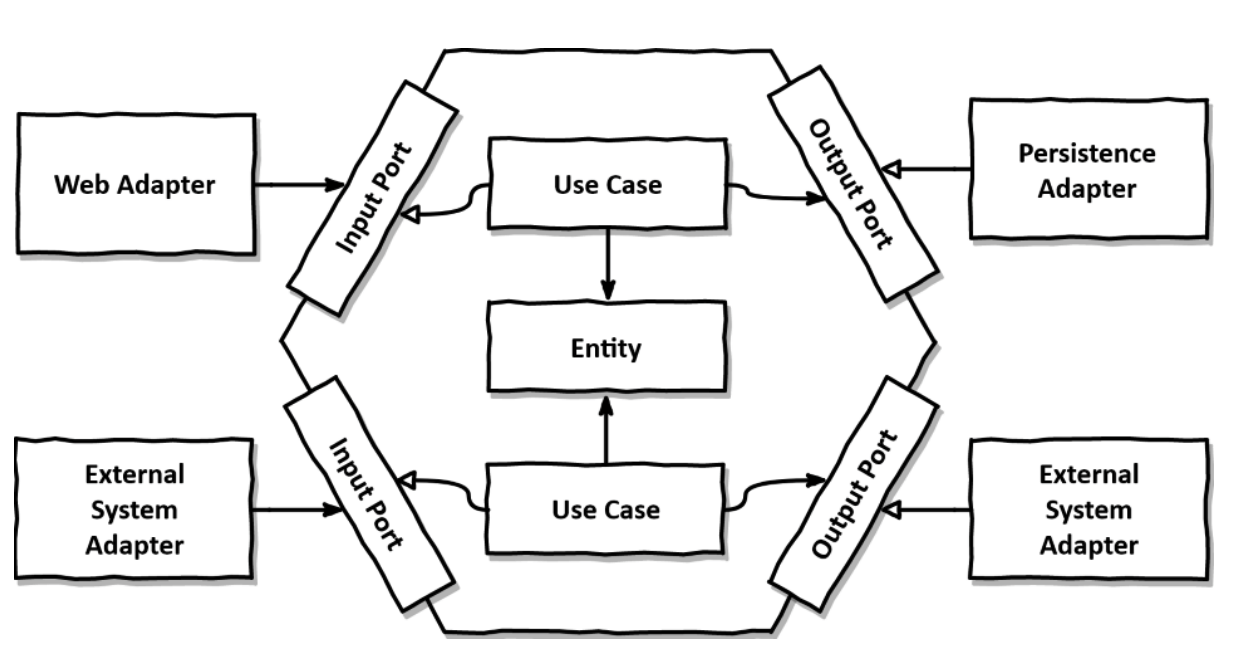
\includegraphics[height=0.3\textheight]{./part/Ejecucion/Seguimiento/CreateTaskUseCase/img/HexagonalDiagram}
%    \caption{Hexagonal architecture diagram\cite{TomHombergs2019GYHD}}\label{fig:hexagonalDiagram}
%\end{figure}

Tomando como referencia \ref{fig:hexagonalDiagram} el diagrmaa tipico de una arquitectura hexagonal, en nuestro caso si intercambiamos ExternalSystemAdapter por nuestro Dispatcher de eventos e introducimos servicios de dominio entre el caso de uso y la Entidad tendremos nuestro esquema de alto nivel de nuestra arquitectura hexagonal. El esbozo de este diagrama lo podemos encontrar en la figura\ref{fig:CreateTaskHexagonalDiagram} Como vemos no tiene tanto sentido el dibujo ya que hay puertos de salida que se convierten en puertos de entrada como es el dispatcher y cuando queremos quitar lógica de negocio del caso de uso mediante servicios de dominio que impidan el acceso directo a los repositorios de persistencia dicho diagrama se va quedando pequeño. Es perferible diagramas UML tal y comose muestra en\ref{fig:createTaskUseCaseArchitecture}


\begin{figure}[H]
    \centering
    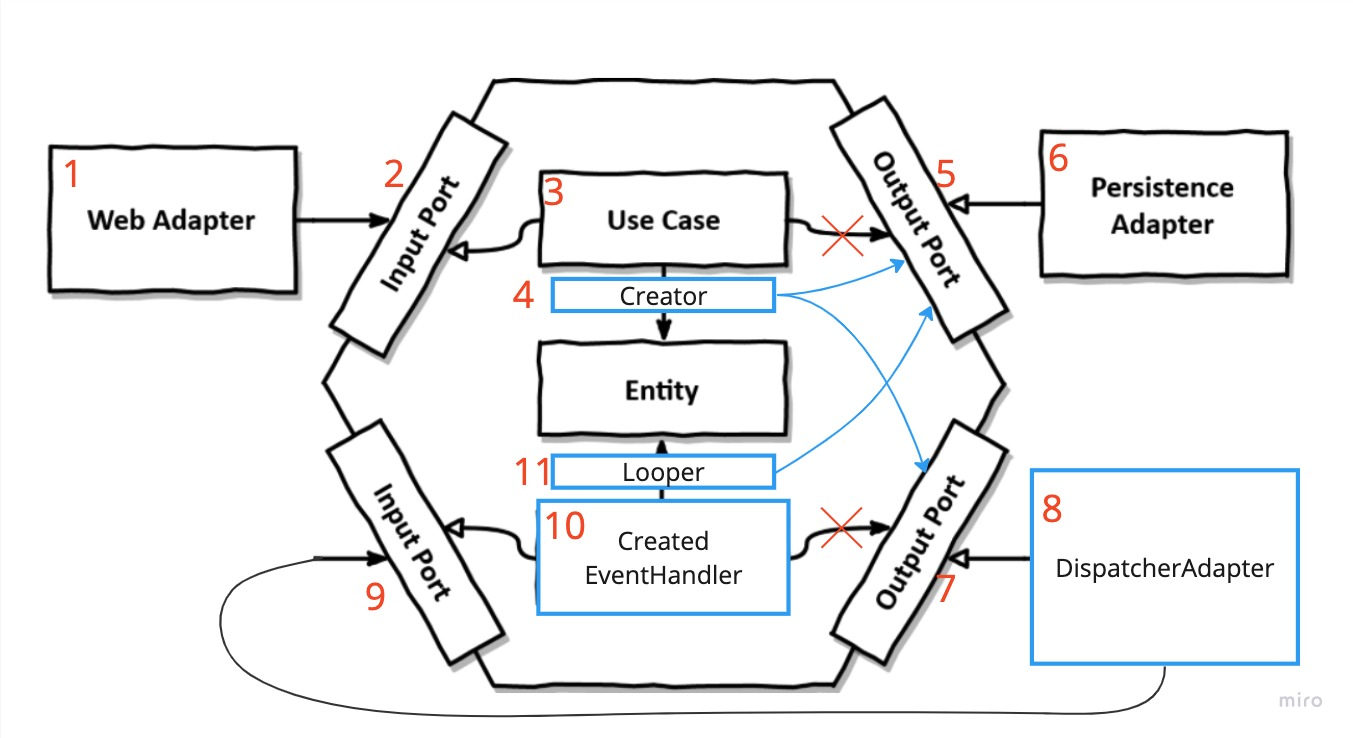
\includegraphics[height=0.3\textheight]{./part/Ejecucion/Seguimiento/CreateTaskUseCase/img/CreateTaskHexagonalDiagram}
    \caption{Hexagonal architecture diagram}\label{fig:CreateTaskHexagonalDiagram}
\end{figure}

\begin{figure}[H]
    \centering
    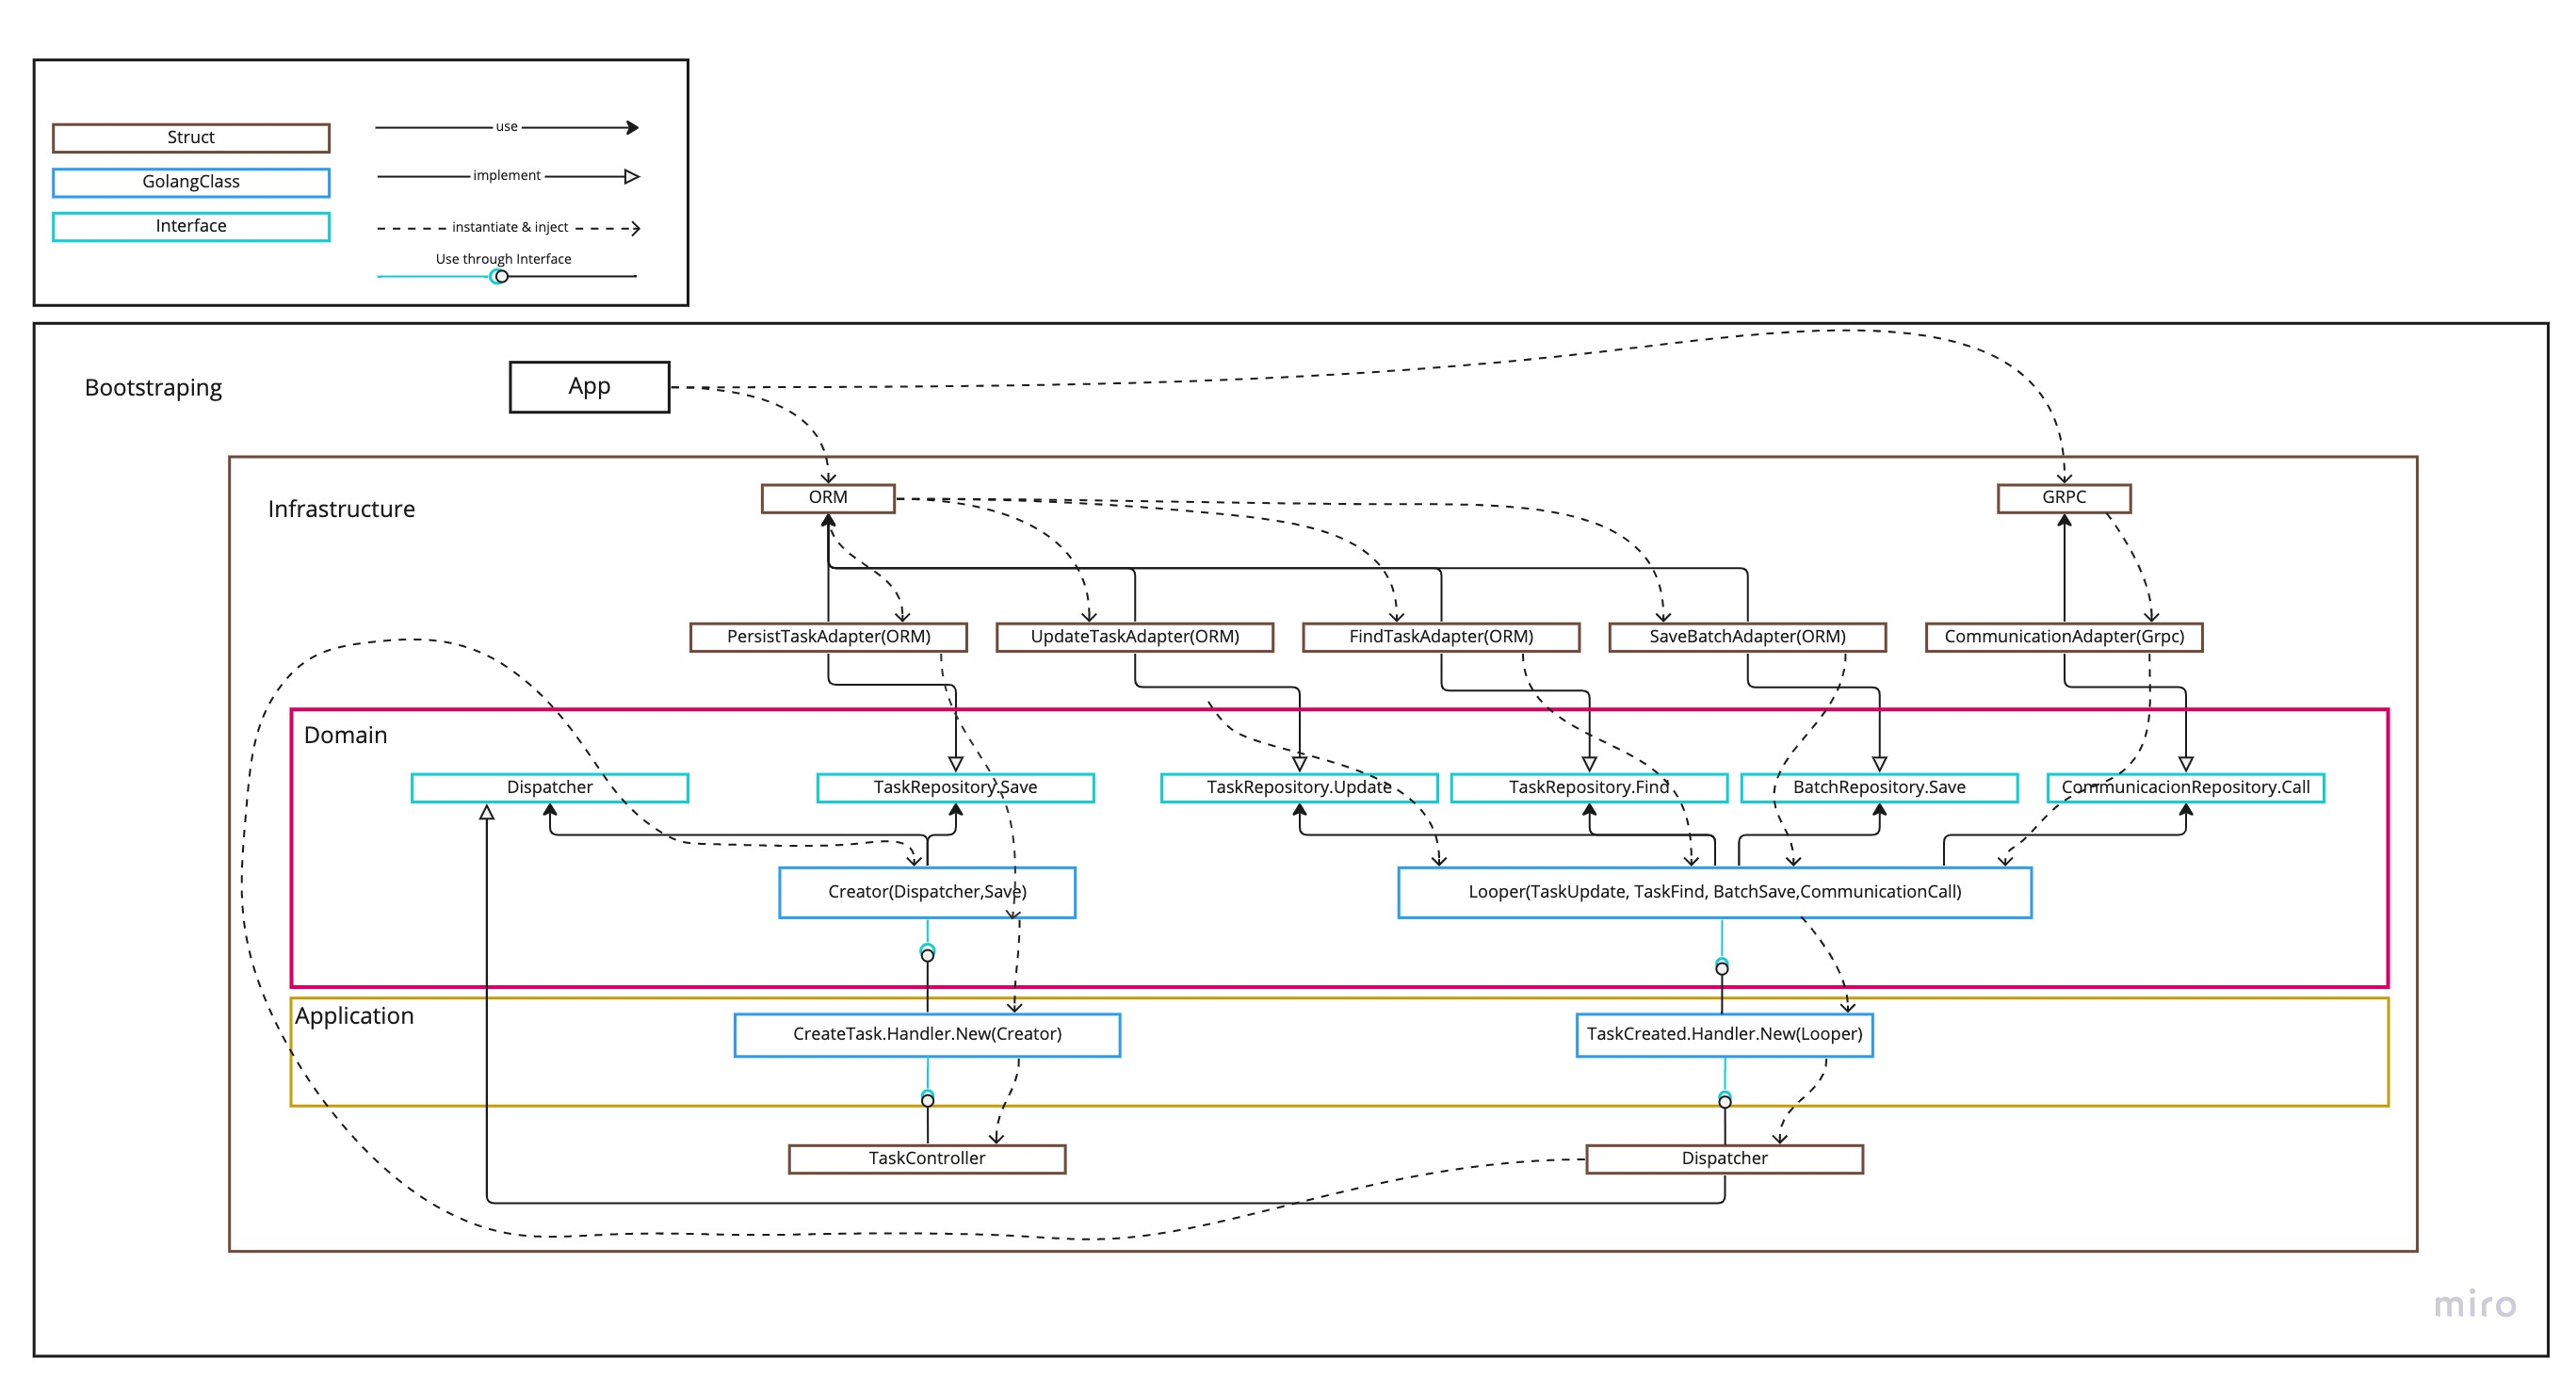
\includegraphics[height=0.3\textheight]{./part/Ejecucion/Seguimiento/CreateTaskUseCase/img/createTaskUseCaseArchitecture}
    \caption{CreateTaskUseCase hexagonal architecture diagram}\label{fig:createTaskUseCaseArchitecture}
\end{figure}

Acercandonos más al código podemos ver en el diagrama \ref{fig:createTaskUseCaseArchitectureFolderStructure} cómo es el uso entre los componentes que exísten en la estructrura de carpetas.

\begin{figure}[H]
    \centering
    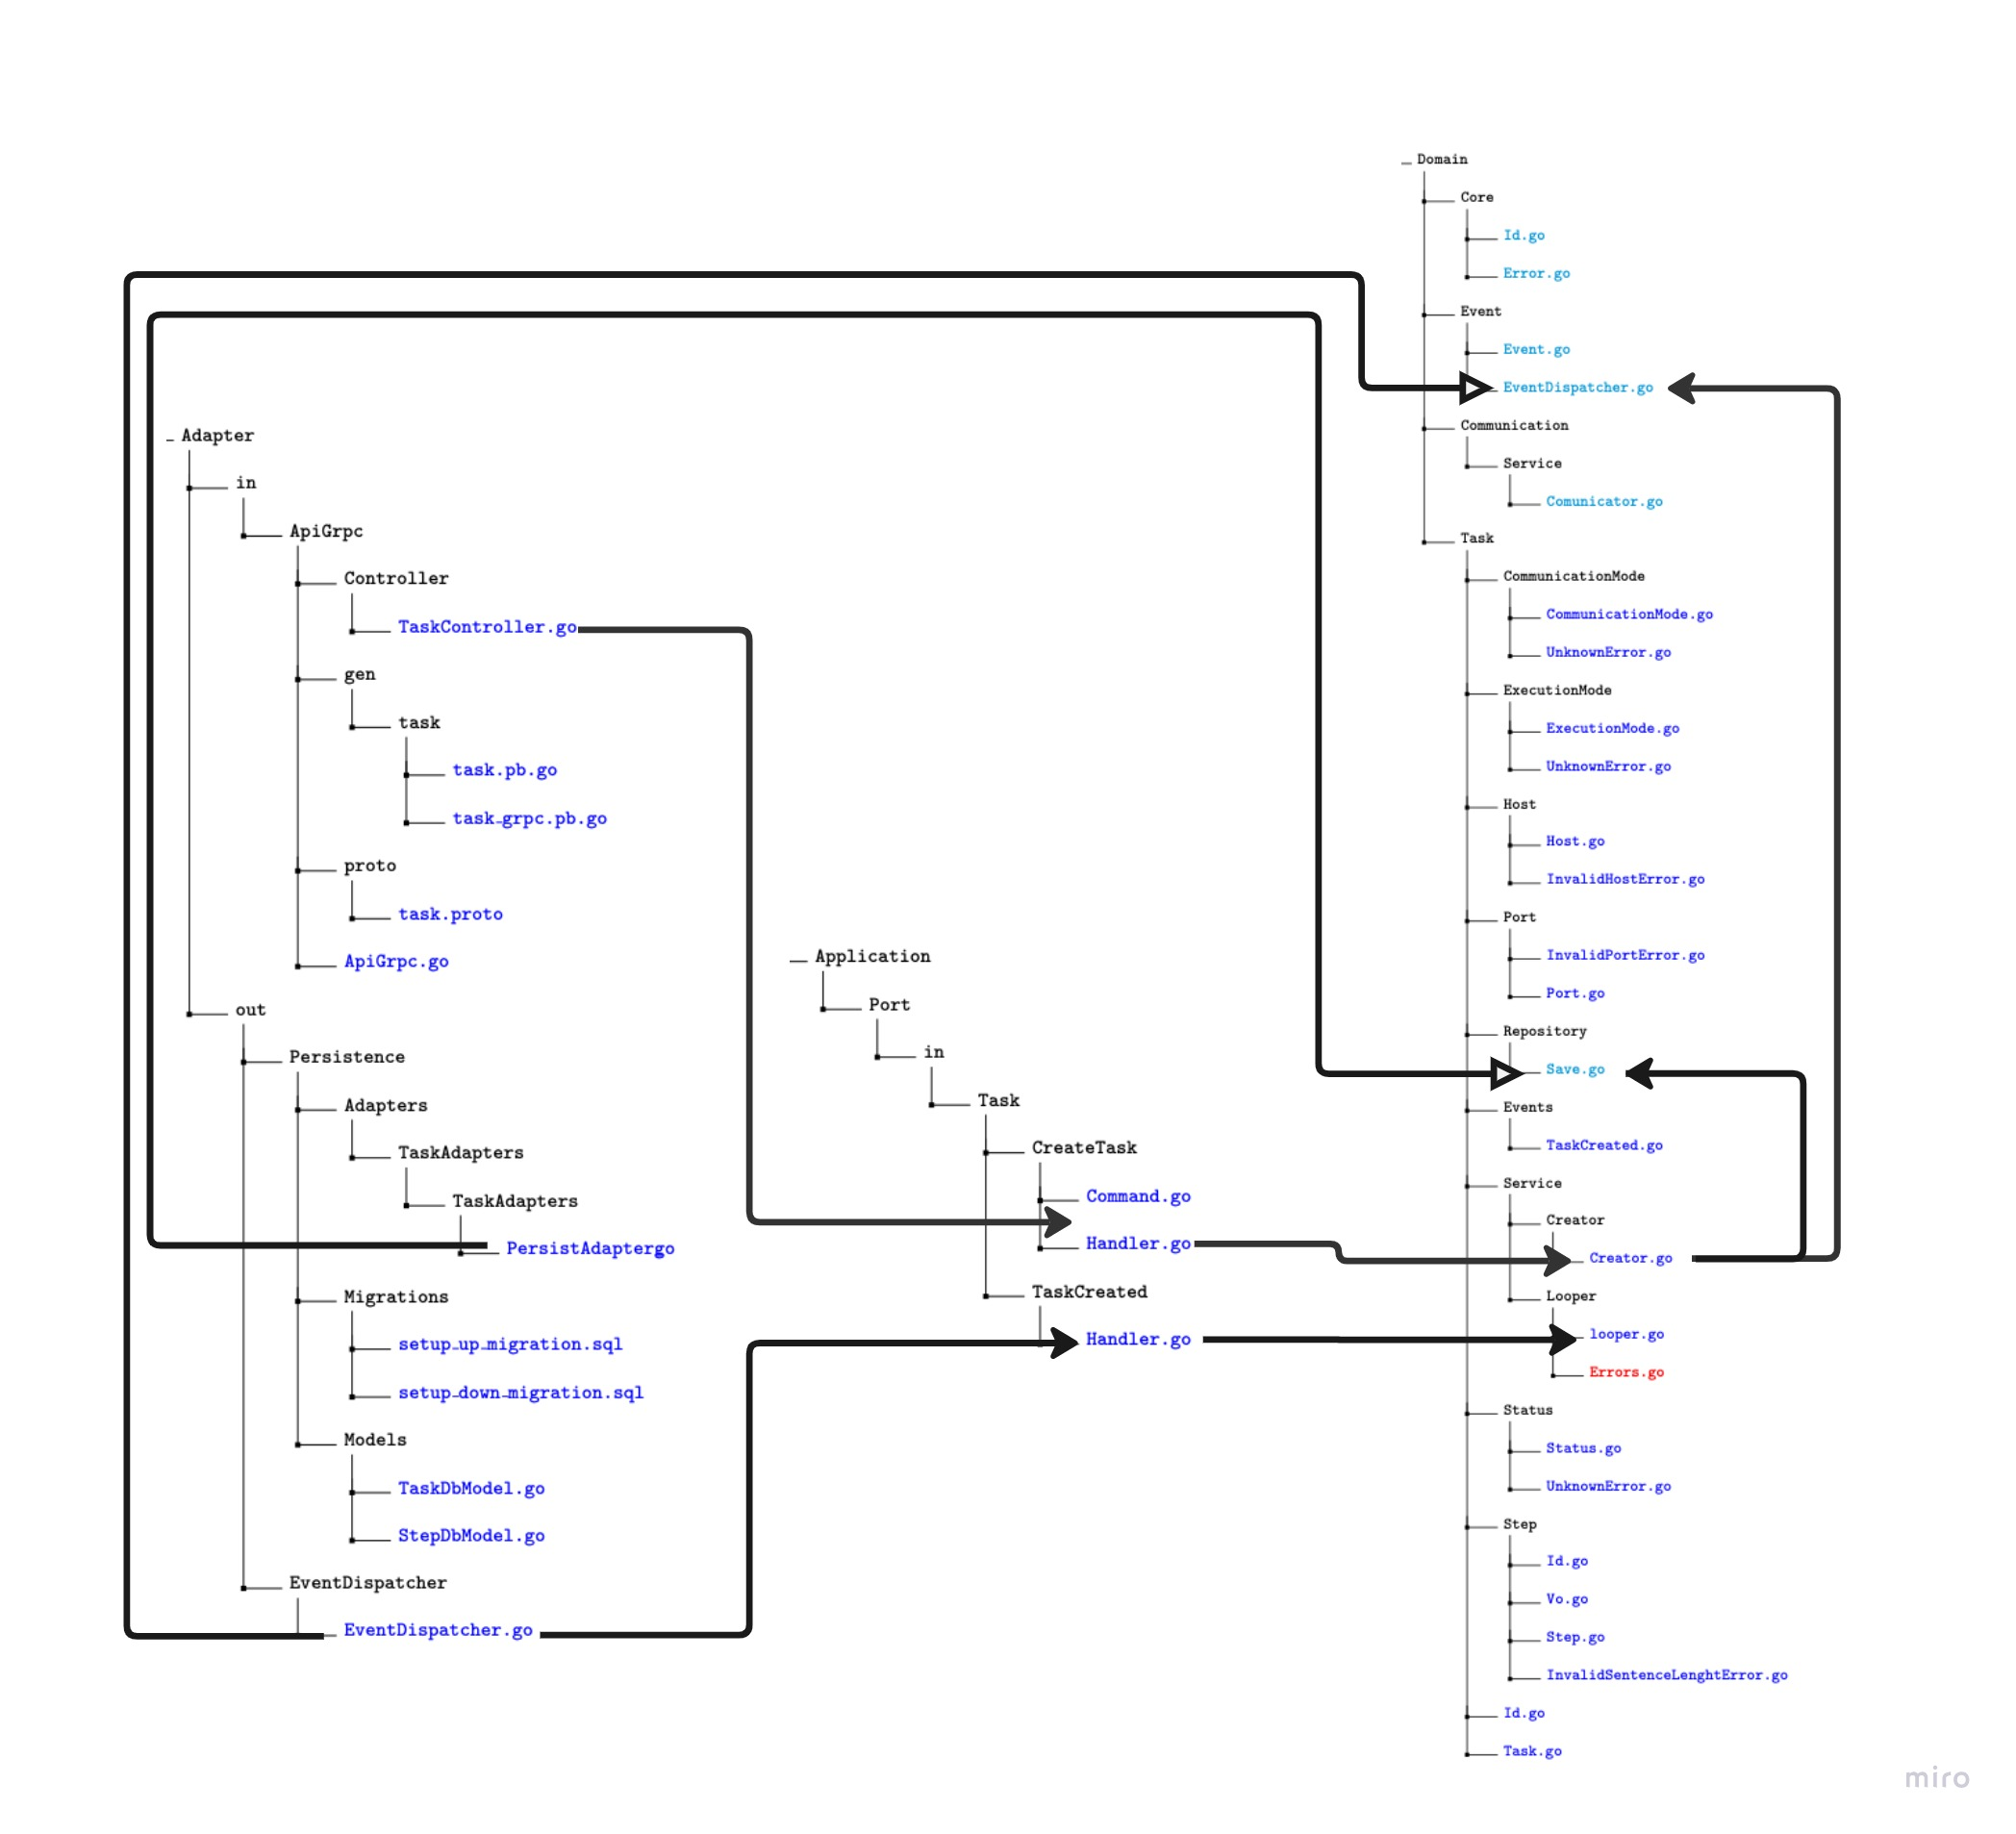
\includegraphics[height=0.5\textheight]{./part/Ejecucion/Seguimiento/CreateTaskUseCase/img/PFM - CreateUseCaseFolderStructure}
    \caption{CreateTaskUseCase folder Structure}\label{fig:createTaskUseCaseArchitectureFolderStructure}
\end{figure}

%Un punto interesante a comentar es el concepto de la estrategia de mapping que hay entre capas. Cada capa requiere sus objetos de trabajo. Tal y como sale descrito en \cite{TomHombergs2019GYHD} Tenemos tantas estratégias como atajos dentro de este paradigma queramos asumir. podemos ver en la figura \ref{fig:mapping types} Los tipos de mapping que se documentan en este libro:
%\begin{itemize}
%    \item The NoMapping Strategy
%    \item The Two-Way MappingStrategy
%    \item The Full MappingStrategy
%    \item The One-Way MappingStrategy
%\end{itemize}

Con respecto a la estrategia de mapping Golang nos permite hacer un full strategy casi por defecto porque al necesitar la implementaci'on de clase para garantizar la cohesión ya estamos utilizando interfaces para todas las clases. Así que en este caso utilizamos un fullMapping adaptado. lo cierto es que las versiones intermedias son todas las combinaciones posibles.

De cara a decidir extraemos la recomendacion de  \cite{TomHombergs2019GYHD}:"
we might start with a simple strategy that allows us to quickly evolve the code and later move to a more complex one that helps us to better decouple the layers.
In order to decide which strategy to use when, we need to agree upon a set of guidelines within the team. These guidelines should answer the question which mapping strategy should be the first choice in which situation. They should also answer why they are first choice so that we’re able to evaluate if those reasons still apply after some time."

Al final se trata de tomar una decisión en equipo, documentar las razones y ser consistentes. Reevaluar las razones ante un reto que las ponga a prueba y tomar o no la decisión de cambiar la estrategia.

En nuestra opinión dentro de la estrategia fullmapping se debe implementar un modelo tanto de entrada, como ya se contempla, como de salída. Es decir, la respuesta que hay entre cada capa también debe ser mappeada, podemos ver el patrón readptado en la figura \ref{fig:GetHandMapping}

\begin{figure}[H]
    \centering
    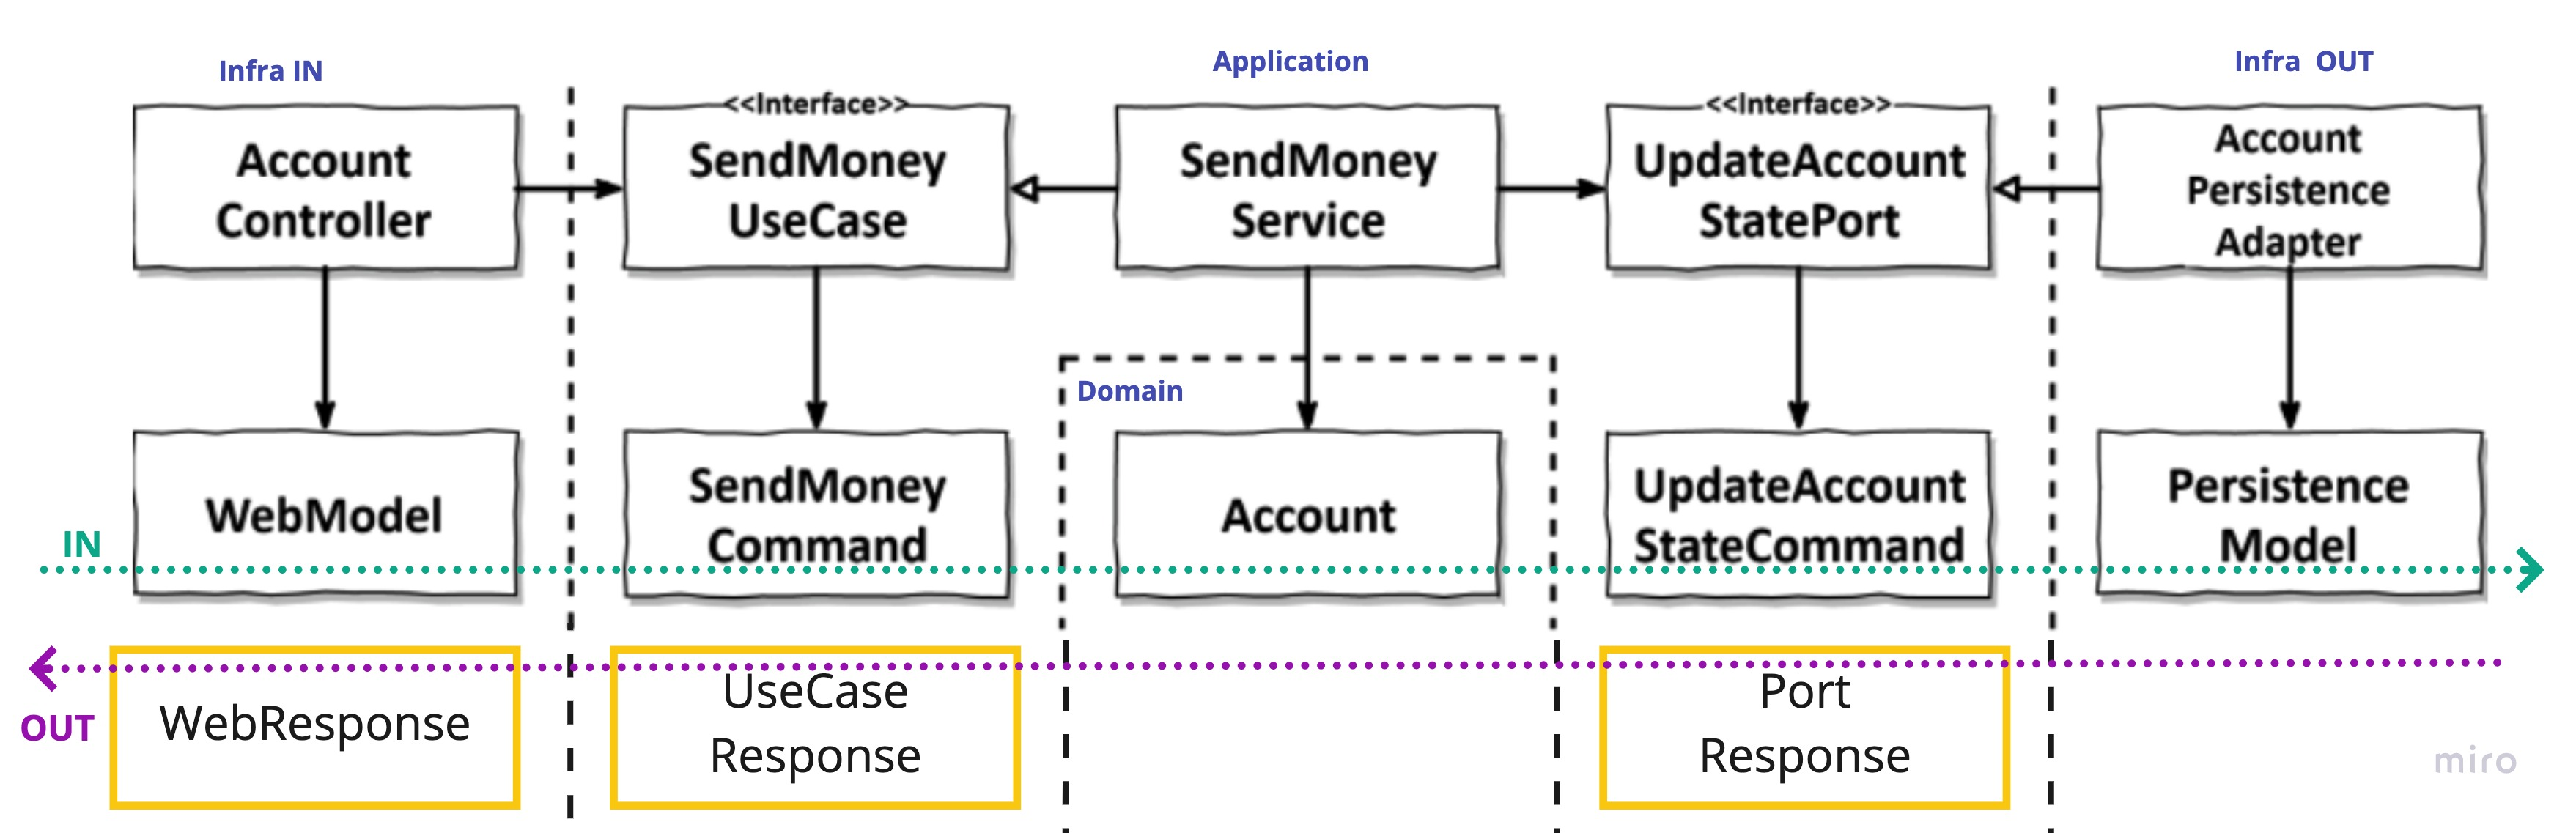
\includegraphics[height=0.2\textheight]{./part/Ejecucion/Seguimiento/CreateTaskUseCase/img/PFM - GetHandMapping}
    \caption{CreateTaskUseCase folder Structure\cite{TomHombergs2019GYHD}}\label{fig:GetHandMapping}
\end{figure}

Claramente esto aumenta la burocracia y finalmente la opción que hemos tomado se puede ver en la figura\ref{fig:CreateTaskUseCaseMapping}

En rojo se han marcado los atajos que se han tomado, es decir, el mapeo que no se ha implementado. El objetivo es aislarse bien de los puertos de entrada, es decir el GRPC, y no tanto de los puertos de salida. ya que la persistencia está bien aislada mediante las interfaces. Dentro de los adaptadores se hará el trabajo de mappeo entre las entidades de dominio y los modelos de persistencia y se traducirá de nuevo a dominio para responder.

\begin{figure}[H]
    \centering
    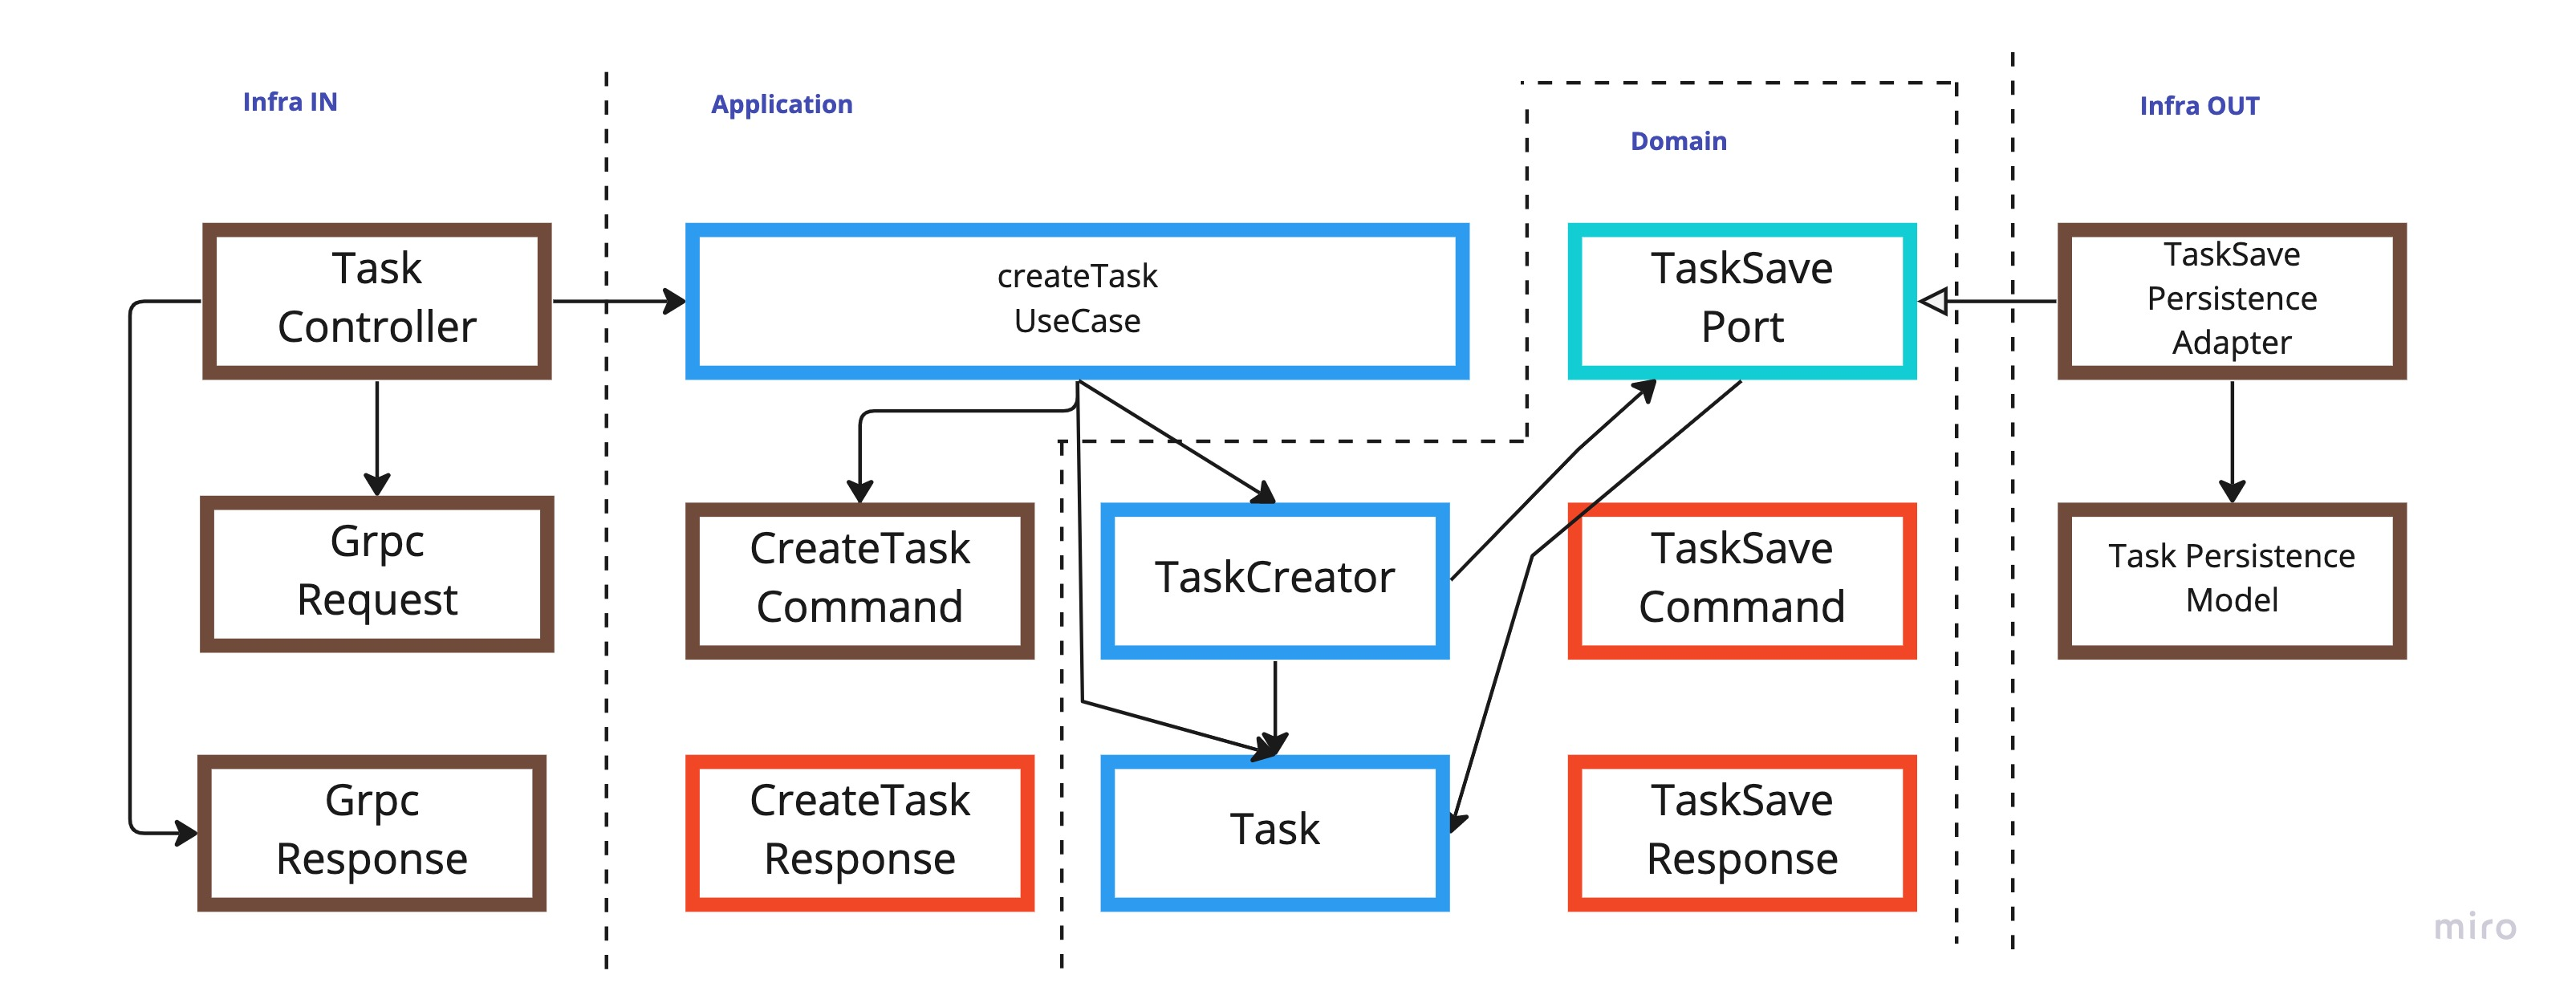
\includegraphics[height=0.2\textheight]{./part/Ejecucion/Seguimiento/CreateTaskUseCase/img/PFM - FinalMapping}
    \caption{CreateTaskUseCase folder Structure}\label{fig:CreateTaskUseCaseMapping}
\end{figure}

Ahora vamos a exponer el código final de este caso de uso, vamos a hacer referencia a:
\begin{itemize}
    \item TaskController \ref{fig:TaskControler}
    \item CreateTaskUseCase \ref{fig:CreateTaskUseCaseCode}
    \item Creator \ref{fig:Creator}
    \item SavePort \ref{fig:SavePort}
    \item PersistAdapter \ref{fig:SaveAdapter}
    \item DispatcherPort \ref{fig:DispatcherPort}
\end{itemize}

\begin{figure}[H]
    \centering
    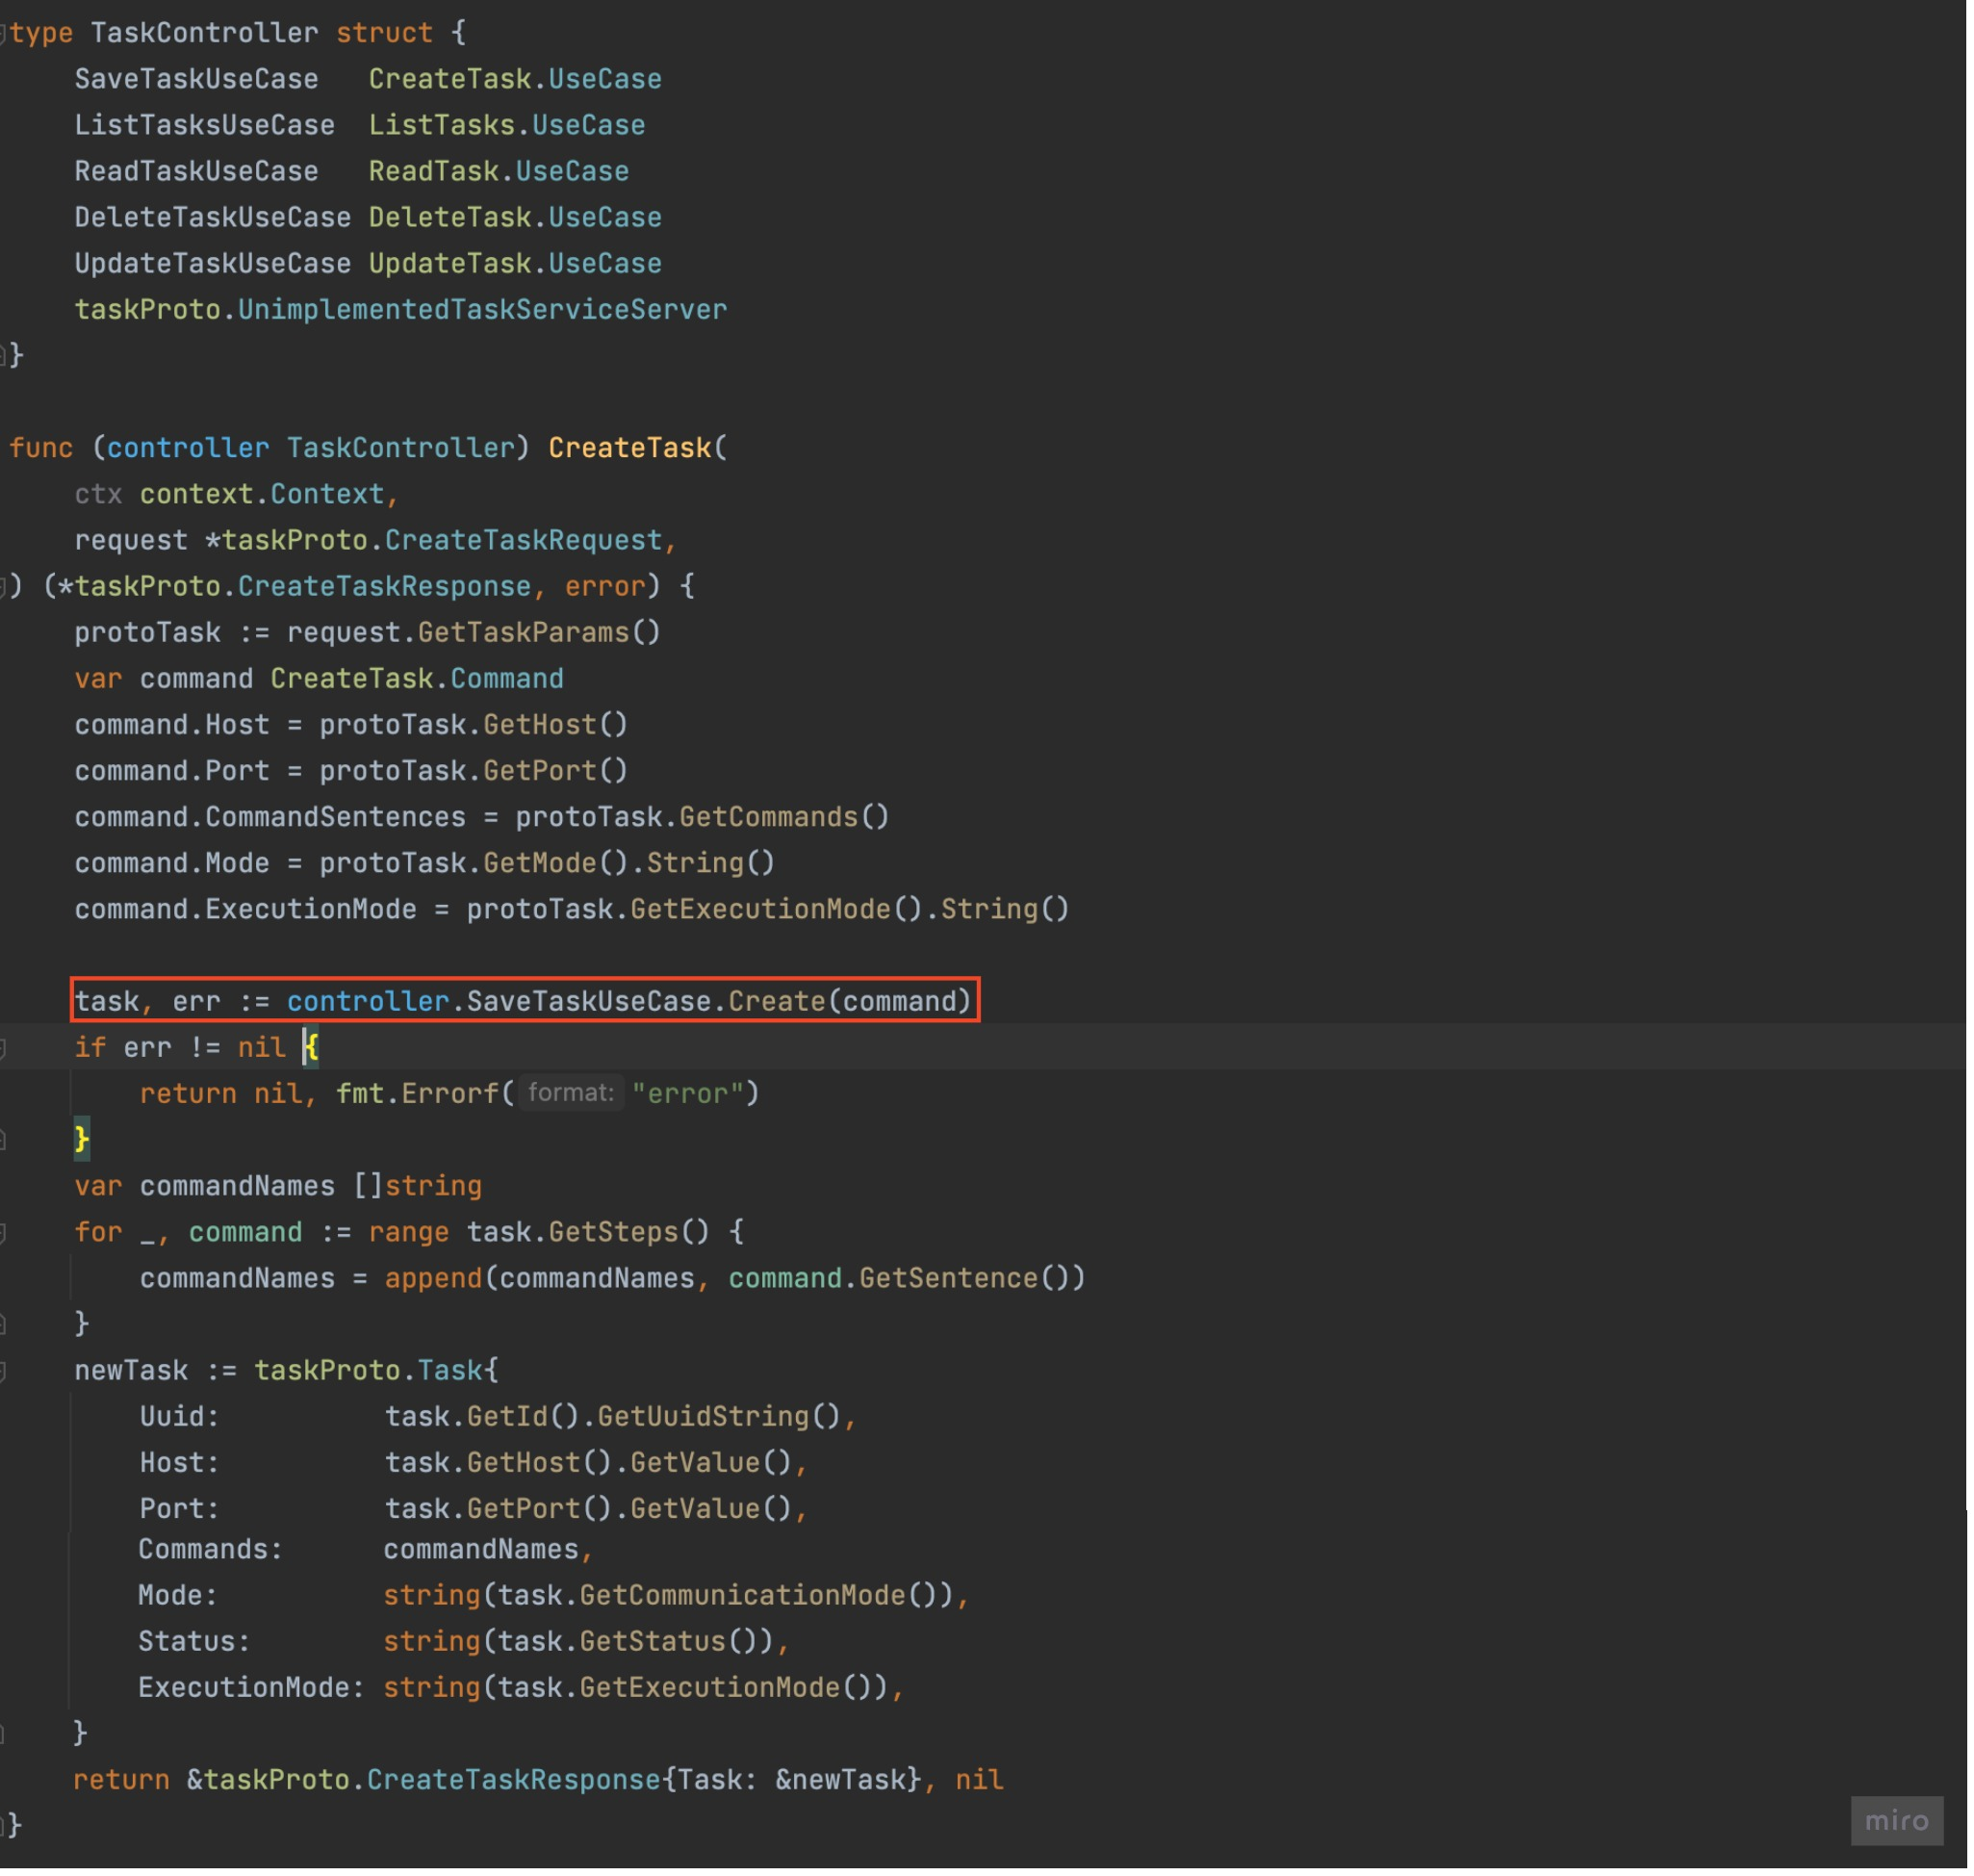
\includegraphics[height=0.5\textheight]{./part/Ejecucion/Seguimiento/CreateTaskUseCase/img/PFM - TaskController}
    \caption{TaskController.go}\label{fig:TaskControler}
\end{figure}

\begin{figure}[H]
    \centering
    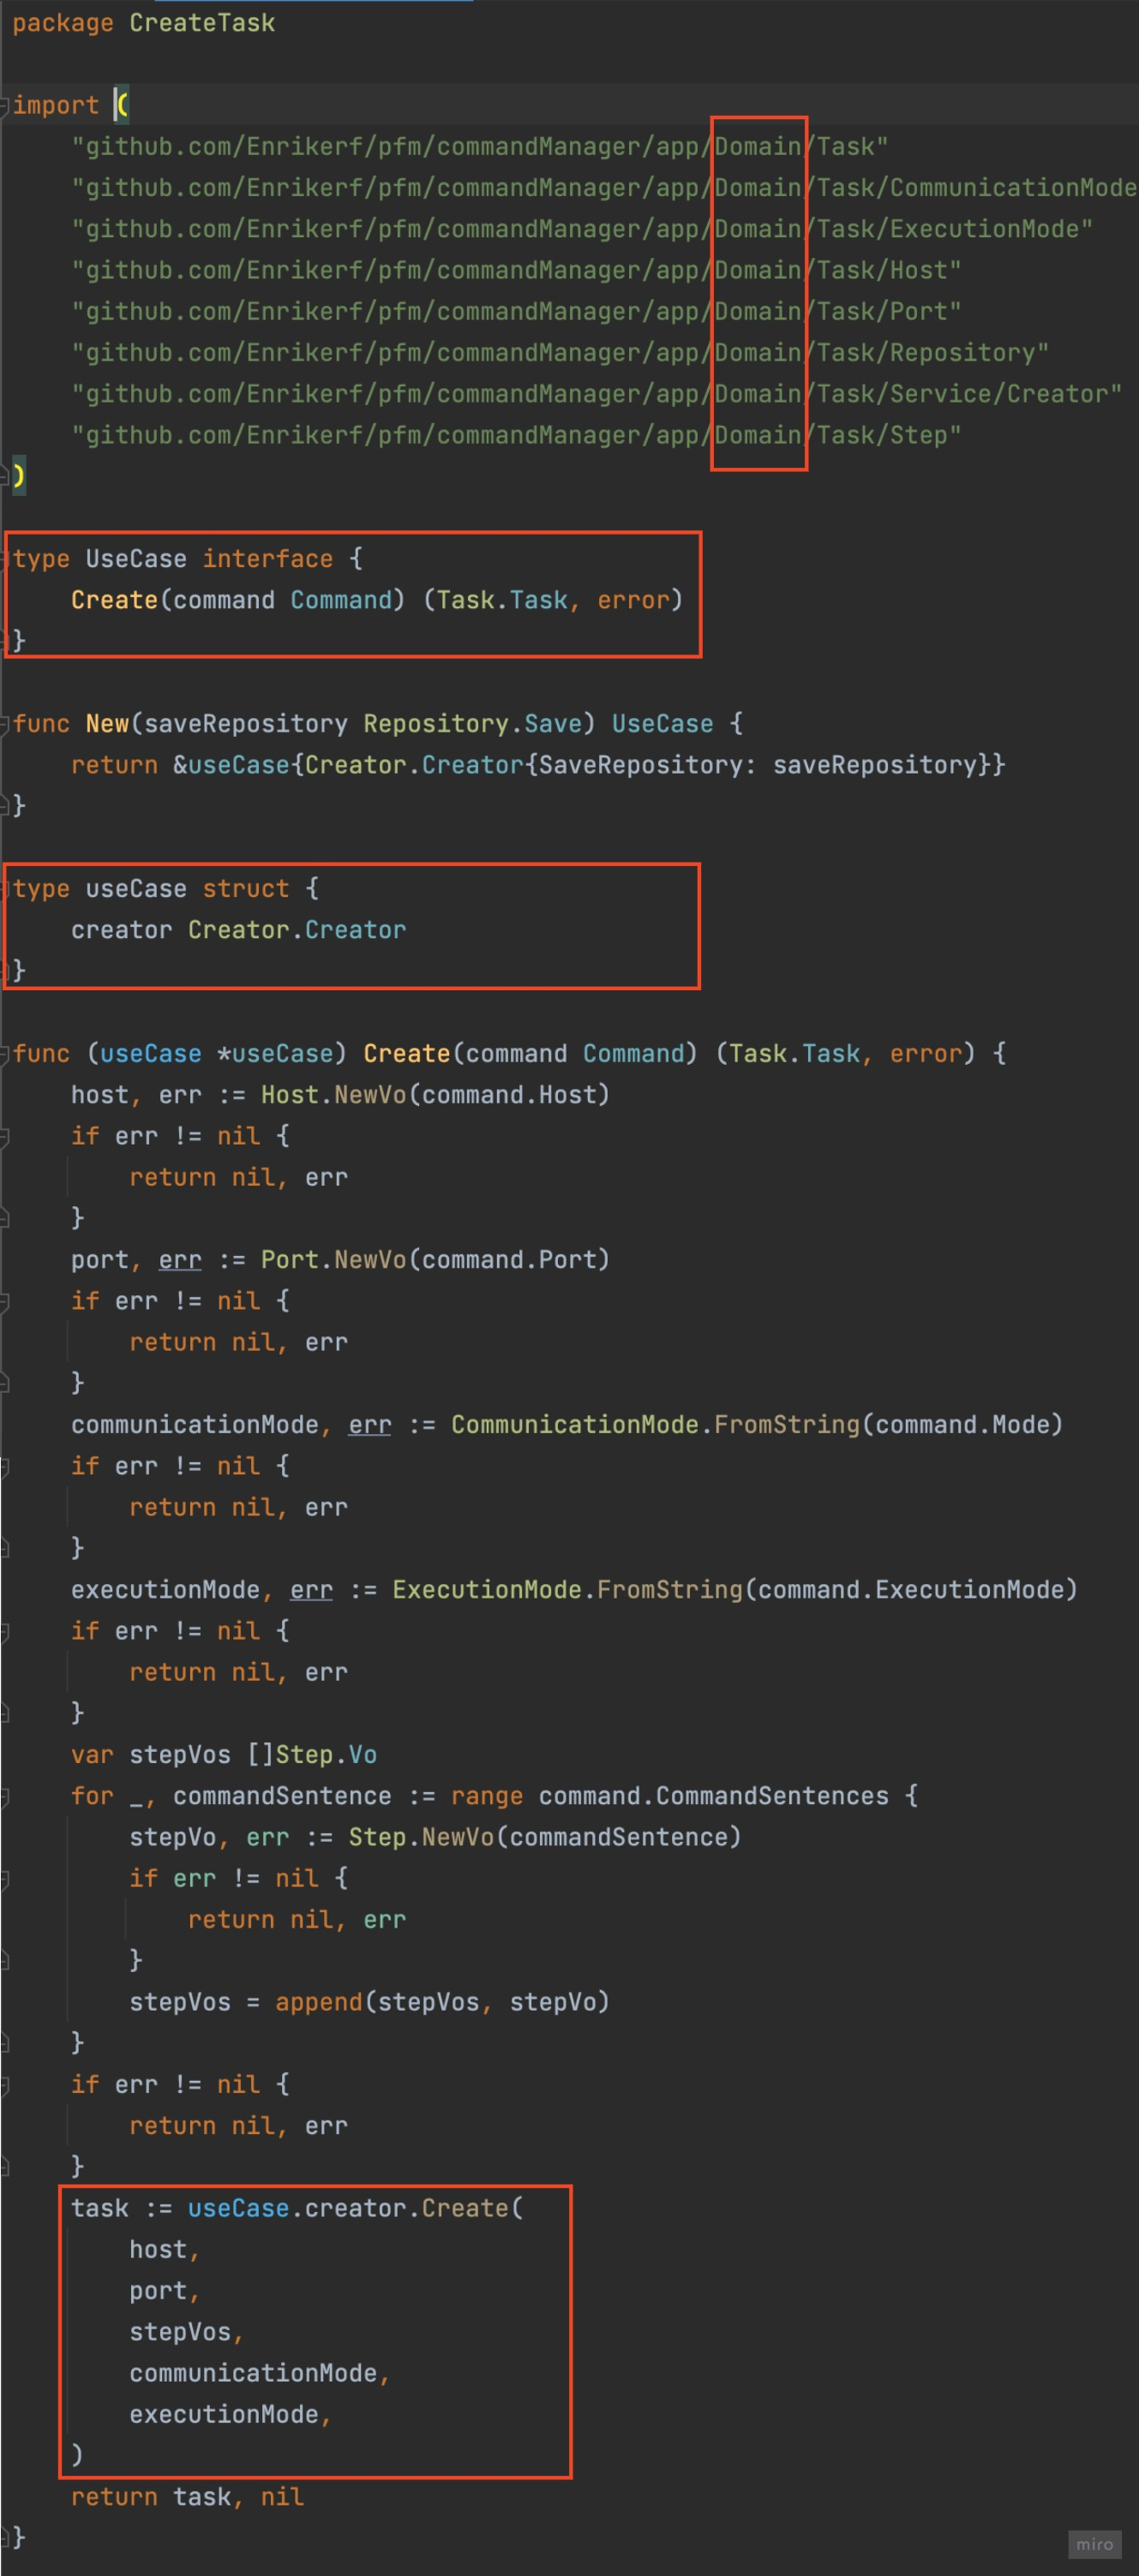
\includegraphics[height=0.5\textheight]{./part/Ejecucion/Seguimiento/CreateTaskUseCase/img/PFM - CreateTaskUseCaseCode}
    \caption{CreateTaskUseCaseCode.go}\label{fig:CreateTaskUseCaseCode}
\end{figure}

\begin{figure}[H]
    \centering
    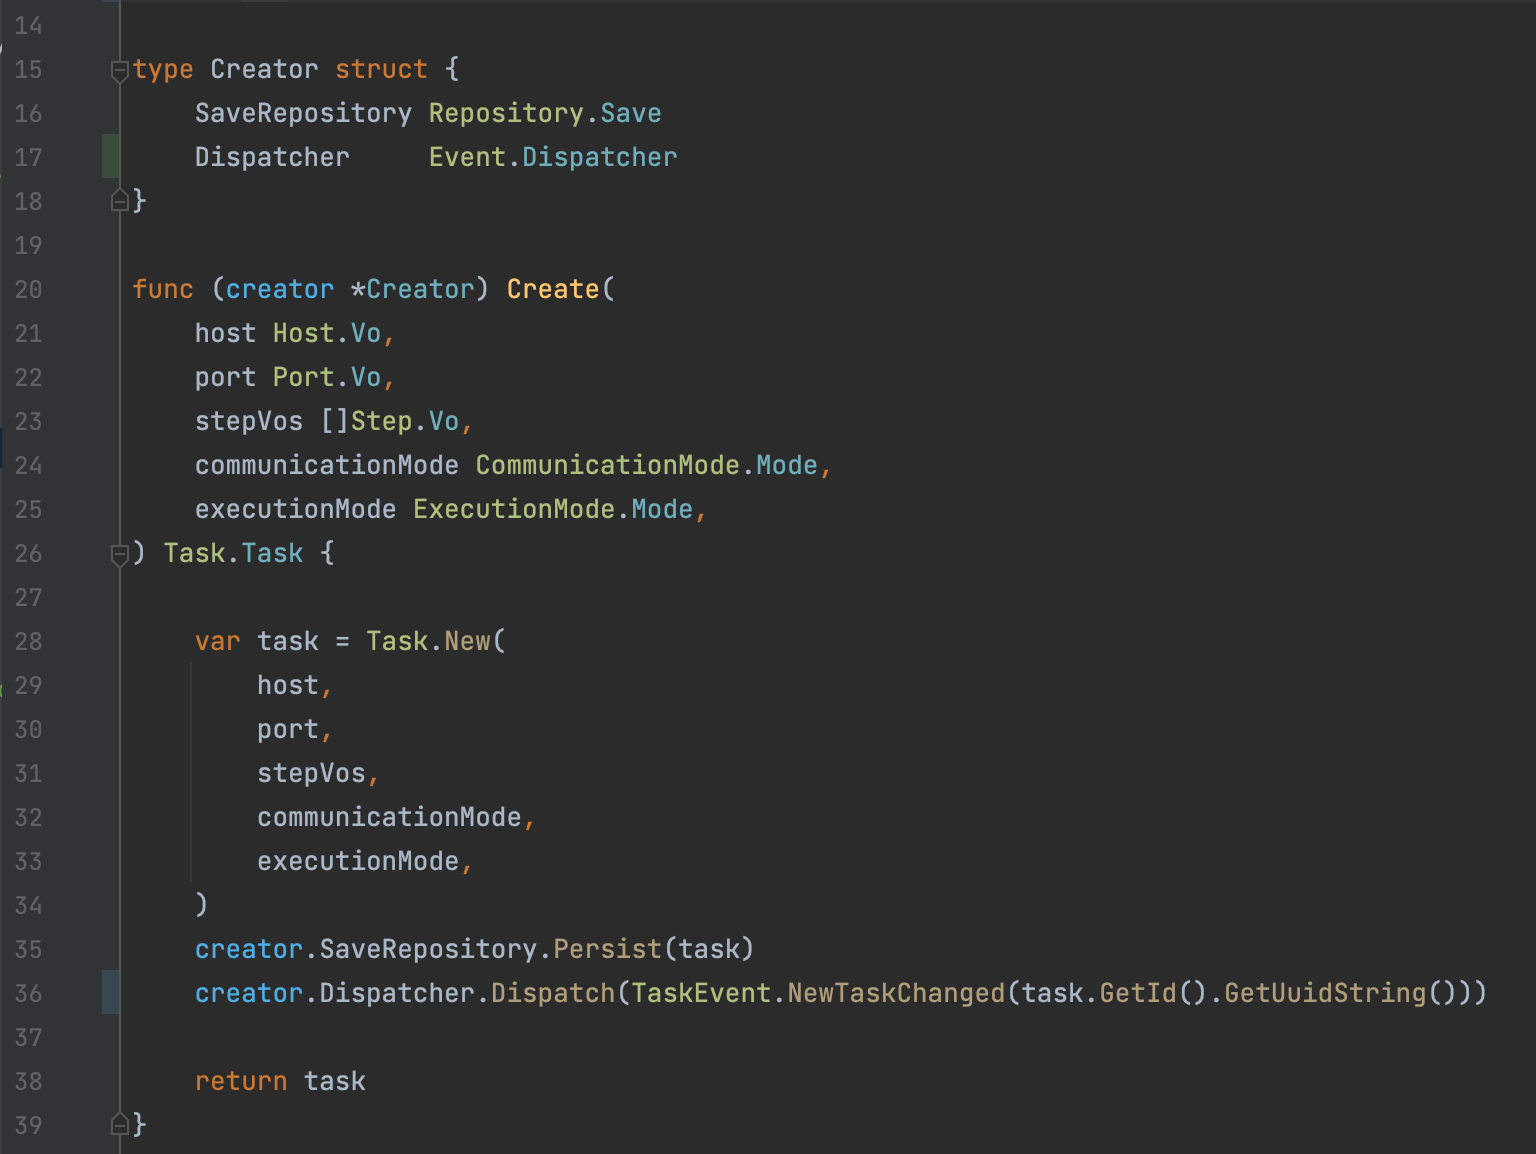
\includegraphics[height=0.5\textheight]{./part/Ejecucion/Seguimiento/CreateTaskUseCase/img/PFM - creator}
    \caption{Creator.go}\label{fig:Creator}
\end{figure}

\begin{figure}[H]
    \centering
    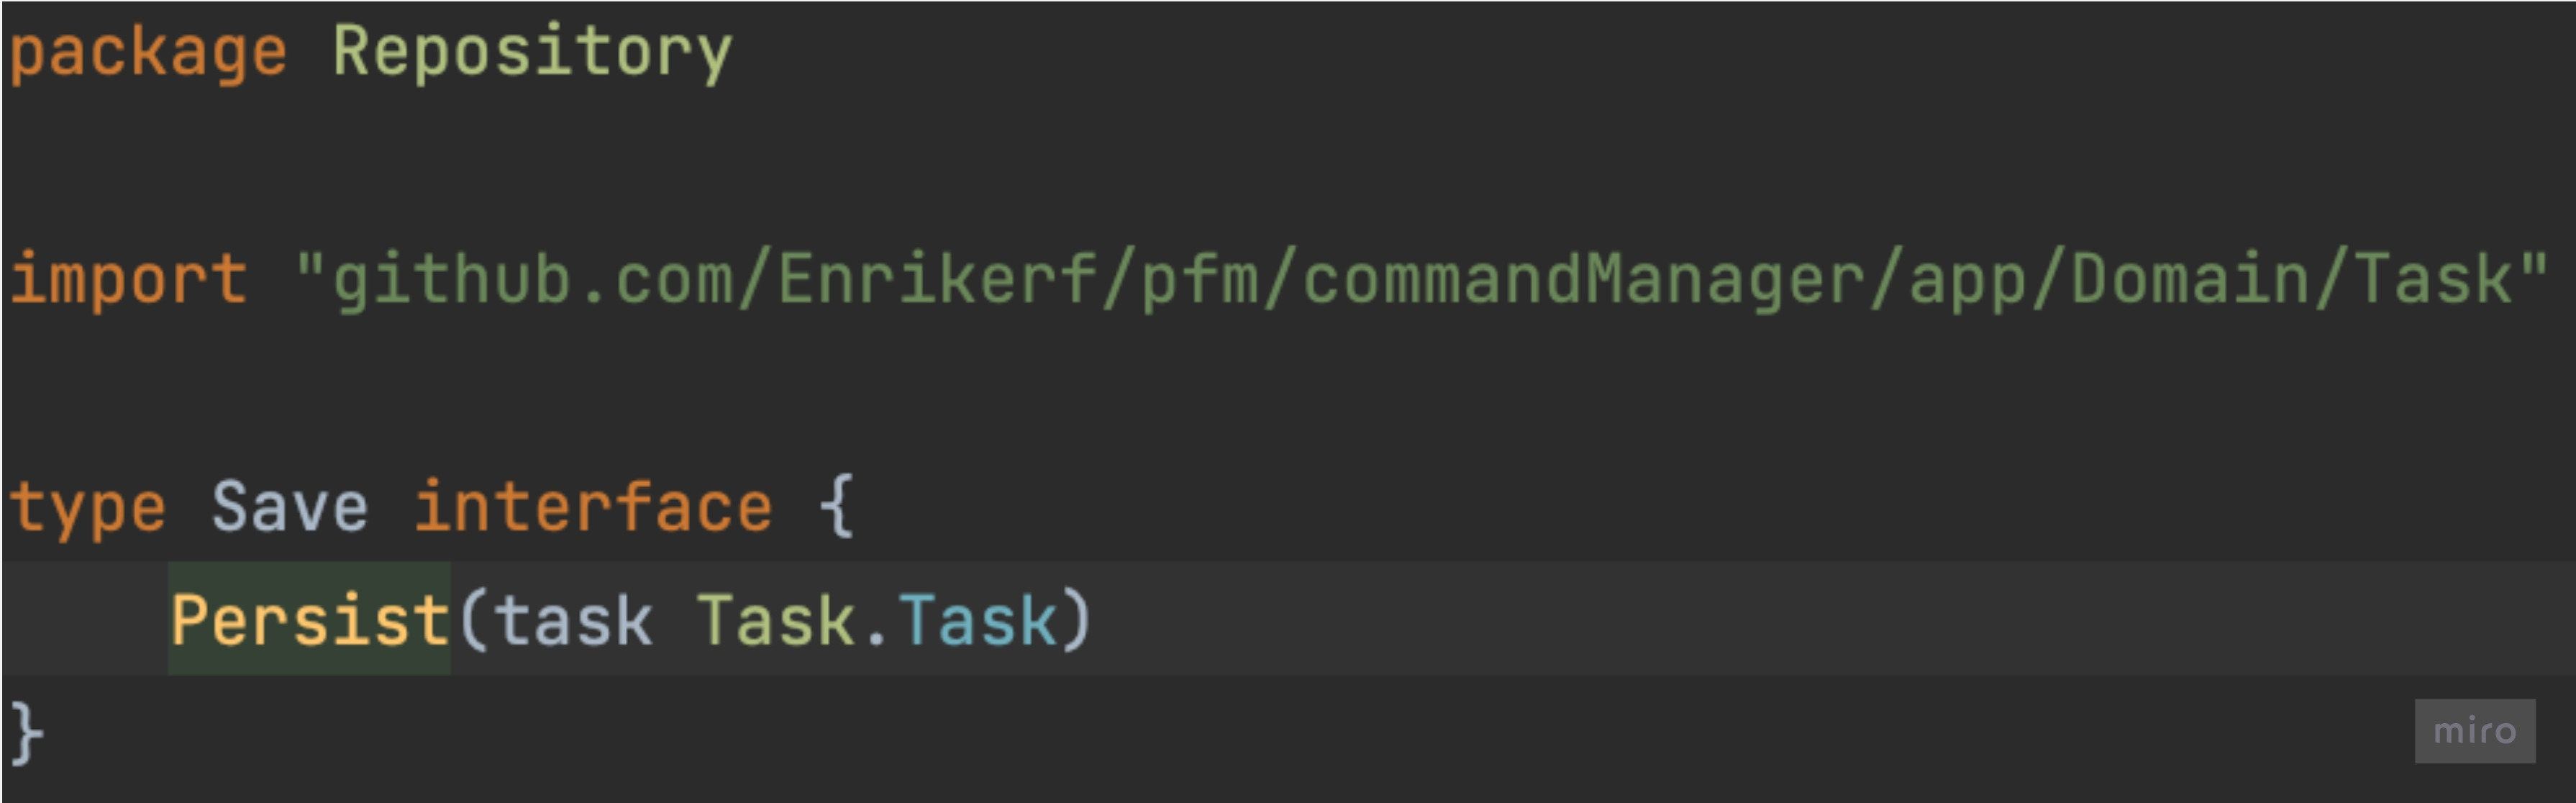
\includegraphics[height=0.2\textheight]{./part/Ejecucion/Seguimiento/CreateTaskUseCase/img/PFM - SavePort}
    \caption{Creator.go}\label{fig:SavePort}
\end{figure}

\begin{figure}[H]
    \centering
    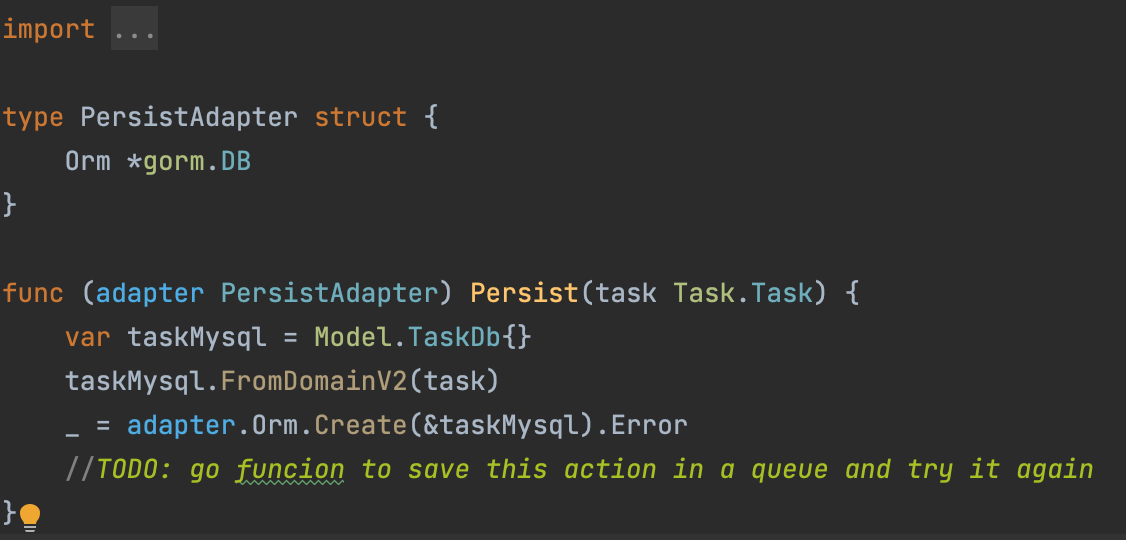
\includegraphics[height=0.2\textheight]{./part/Ejecucion/Seguimiento/CreateTaskUseCase/img/PFM - SaveAdapter}
    \caption{Creator.go}\label{fig:SaveAdapter}
\end{figure}

\begin{figure}[H]
    \centering
    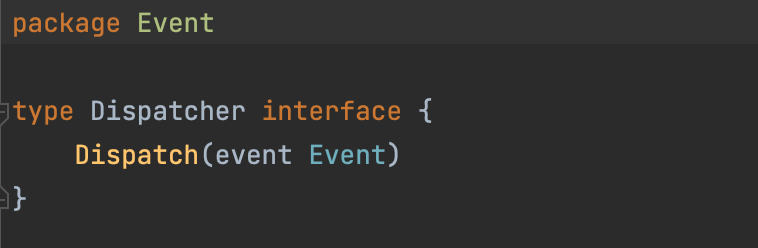
\includegraphics[height=0.2\textheight]{./part/Ejecucion/Seguimiento/CreateTaskUseCase/img/PFM - Dispatcher}
    \caption{Creator.go}\label{fig:DispatcherPort}
\end{figure}
\subsubsection{CallAdapter}
%    
El codigo de colores utilizado en los diagramas de esta seccion se refieren al equivalente a clase en golang en azul y a las interfaces puras en turquesa  y a los structs en marron

%El tipico diagráma cuando se habla de arquitectura hexagonal es tal y como se muestra en la figura\ref{fig:hexagonalDiagram} Si bien consideramos que no tiene mucho sentido y de cara a la parte didáctica confunde, ya que el hexágono es una simple licencia estética. en el caso de existir más puertos de salida y entrada que los representados el hexágono pierde todo el sentido y cuando se enfrenta por primera vez este diagrama se tiende a intentar descifrar el sentído del hexagono.
%
%\begin{figure}[H]
%    \centering
%    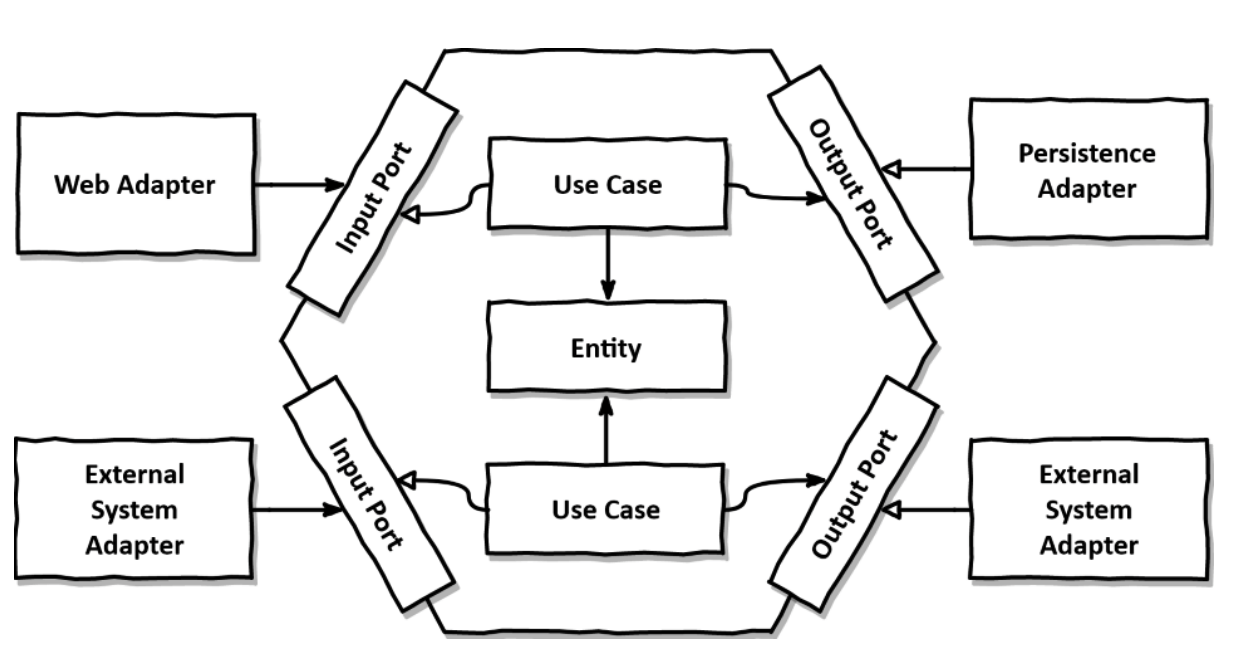
\includegraphics[height=0.3\textheight]{./part/Ejecucion/Seguimiento/CreateTaskUseCase/img/HexagonalDiagram}
%    \caption{Hexagonal architecture diagram\cite{TomHombergs2019GYHD}}\label{fig:hexagonalDiagram}
%\end{figure}

Tomando como referencia \ref{fig:hexagonalDiagram} el diagrmaa tipico de una arquitectura hexagonal, en nuestro caso si intercambiamos ExternalSystemAdapter por nuestro Dispatcher de eventos e introducimos servicios de dominio entre el caso de uso y la Entidad tendremos nuestro esquema de alto nivel de nuestra arquitectura hexagonal. El esbozo de este diagrama lo podemos encontrar en la figura\ref{fig:CreateTaskHexagonalDiagram} Como vemos no tiene tanto sentido el dibujo ya que hay puertos de salida que se convierten en puertos de entrada como es el dispatcher y cuando queremos quitar lógica de negocio del caso de uso mediante servicios de dominio que impidan el acceso directo a los repositorios de persistencia dicho diagrama se va quedando pequeño. Es perferible diagramas UML tal y comose muestra en\ref{fig:createTaskUseCaseArchitecture}


\begin{figure}[H]
    \centering
    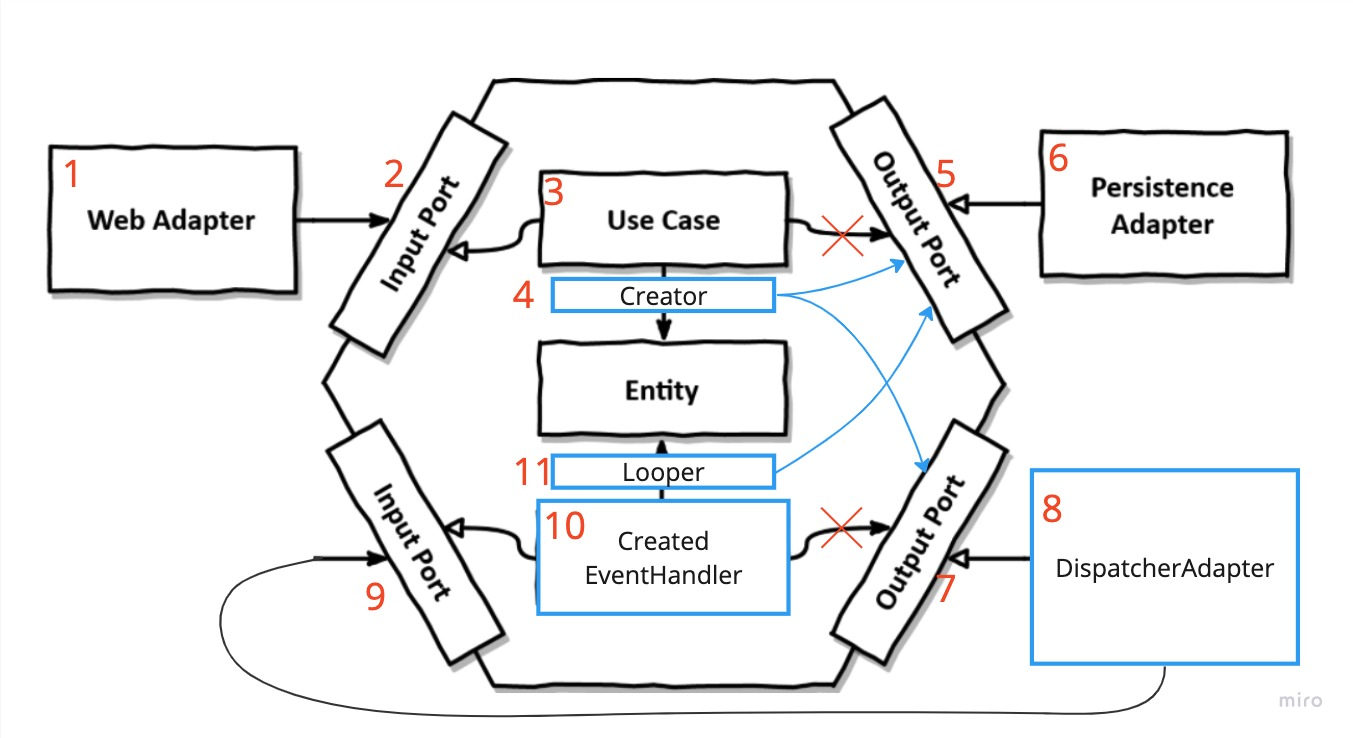
\includegraphics[height=0.3\textheight]{./part/Ejecucion/Seguimiento/CreateTaskUseCase/img/CreateTaskHexagonalDiagram}
    \caption{Hexagonal architecture diagram}\label{fig:CreateTaskHexagonalDiagram}
\end{figure}

\begin{figure}[H]
    \centering
    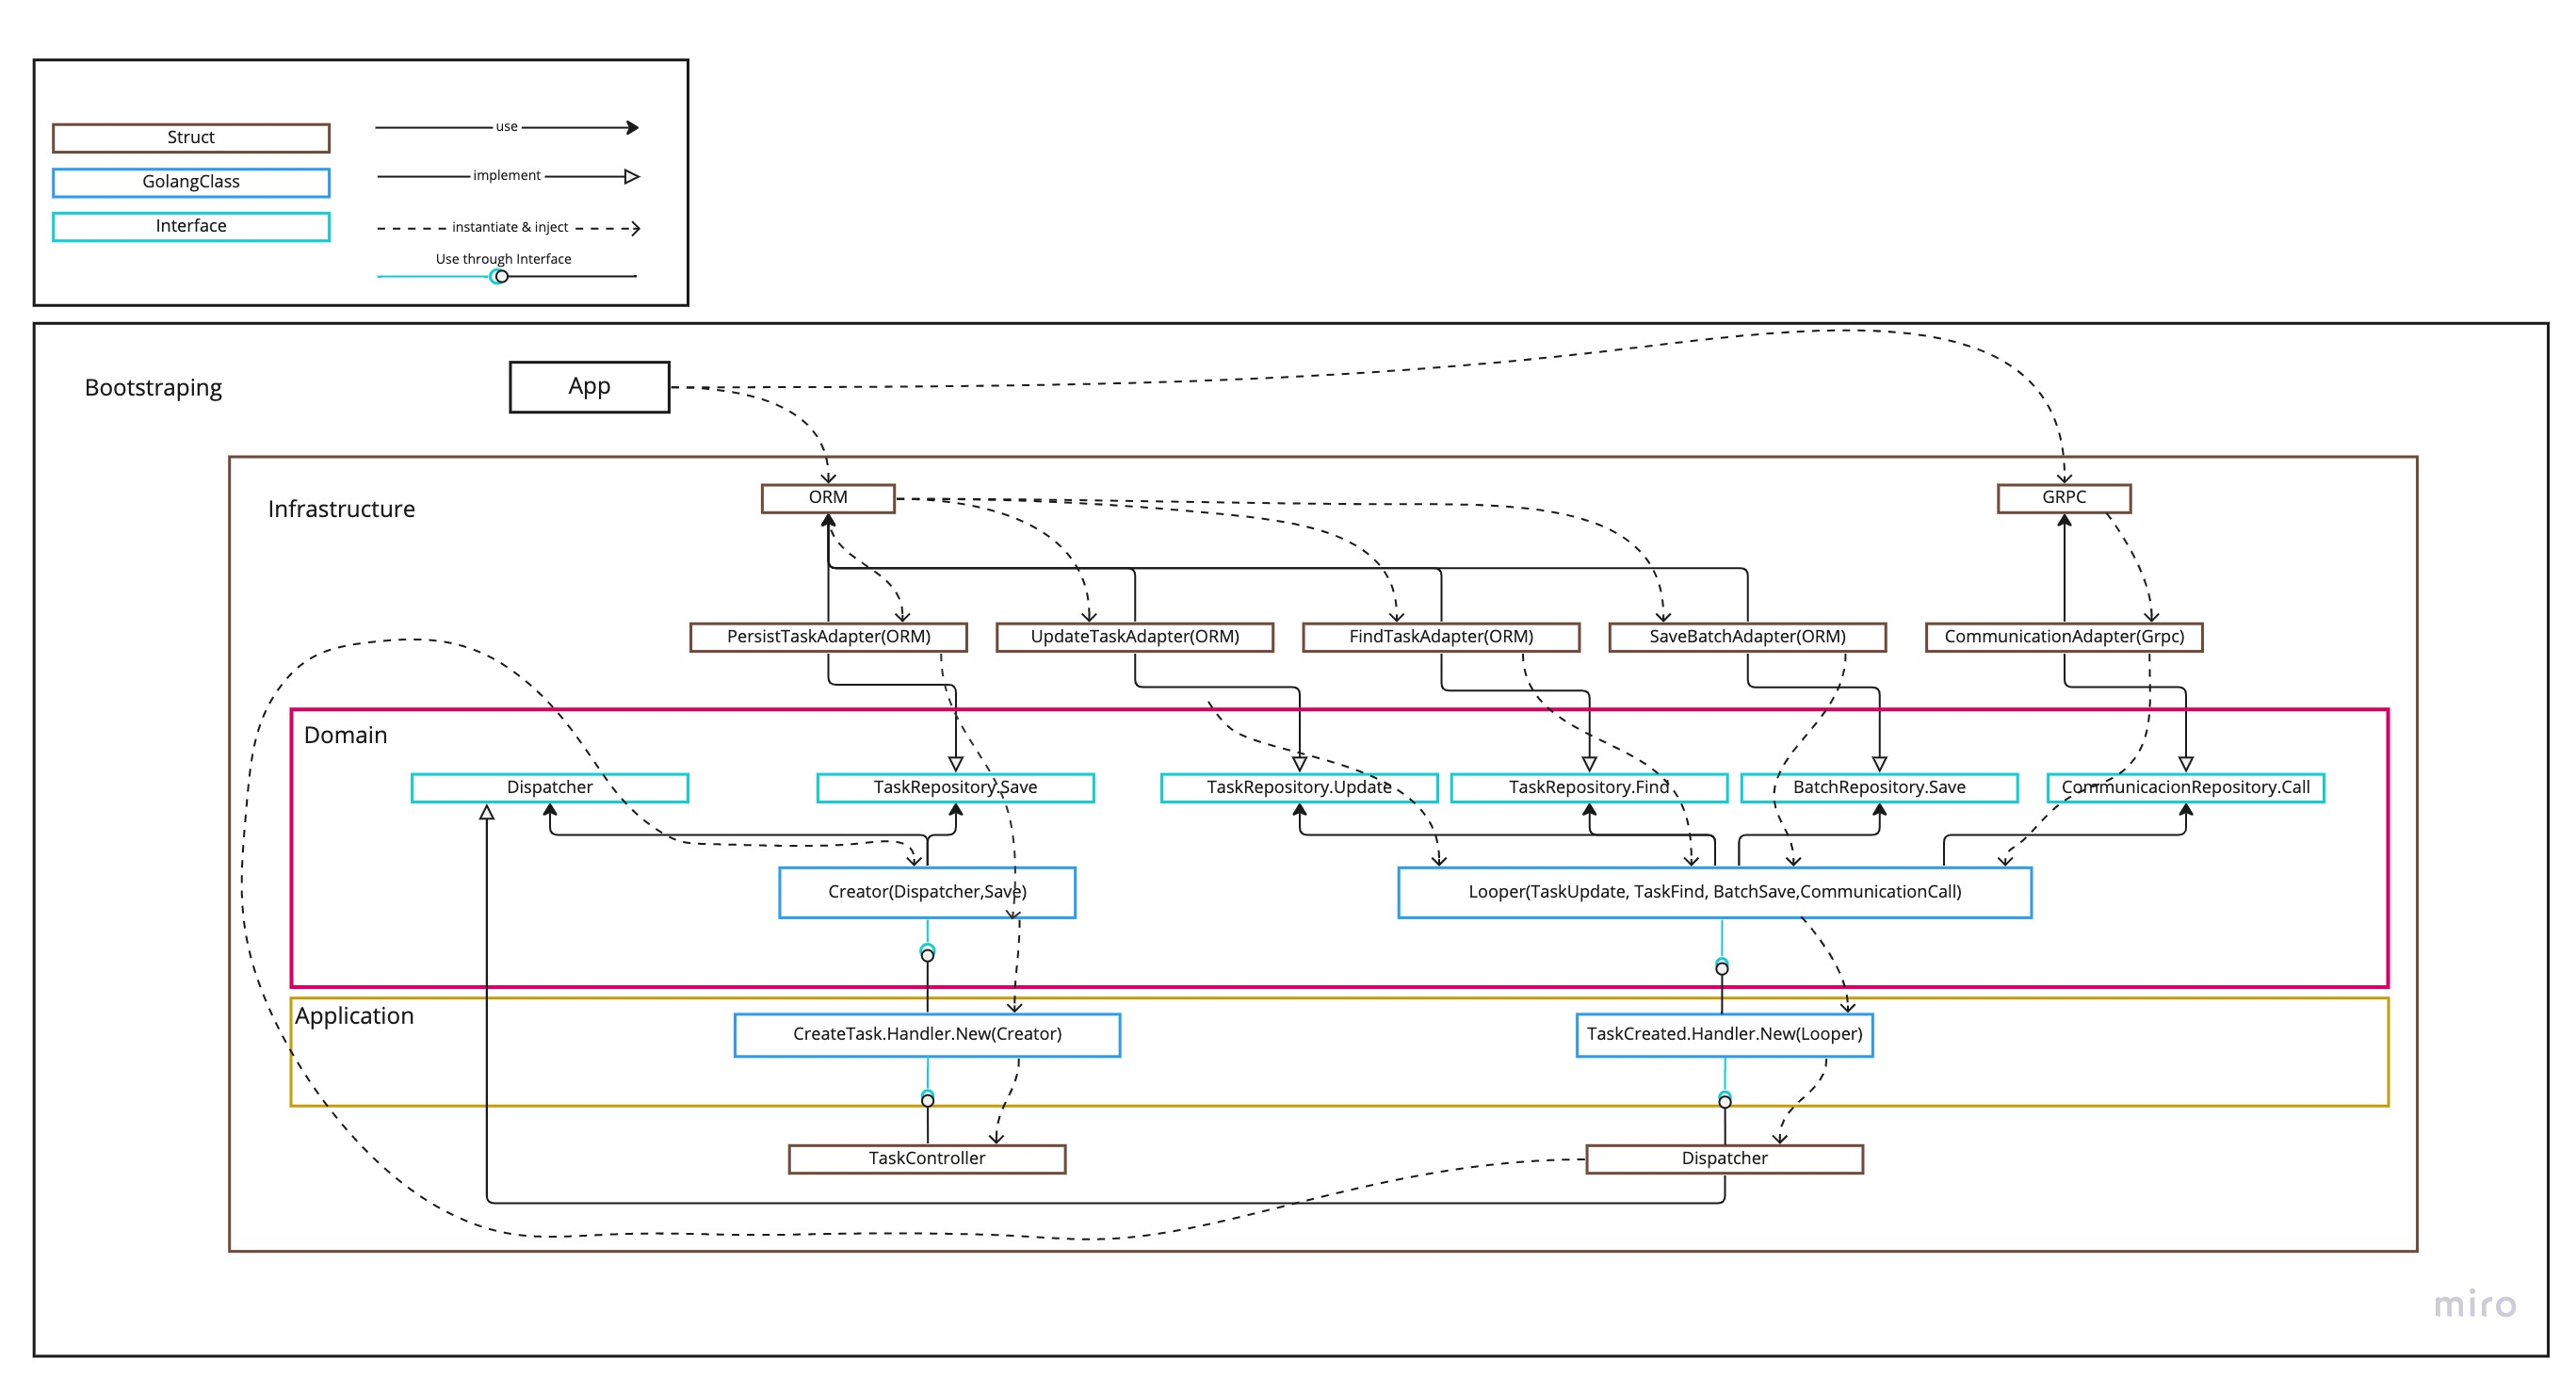
\includegraphics[height=0.3\textheight]{./part/Ejecucion/Seguimiento/CreateTaskUseCase/img/createTaskUseCaseArchitecture}
    \caption{CreateTaskUseCase hexagonal architecture diagram}\label{fig:createTaskUseCaseArchitecture}
\end{figure}

Acercandonos más al código podemos ver en el diagrama \ref{fig:createTaskUseCaseArchitectureFolderStructure} cómo es el uso entre los componentes que exísten en la estructrura de carpetas.

\begin{figure}[H]
    \centering
    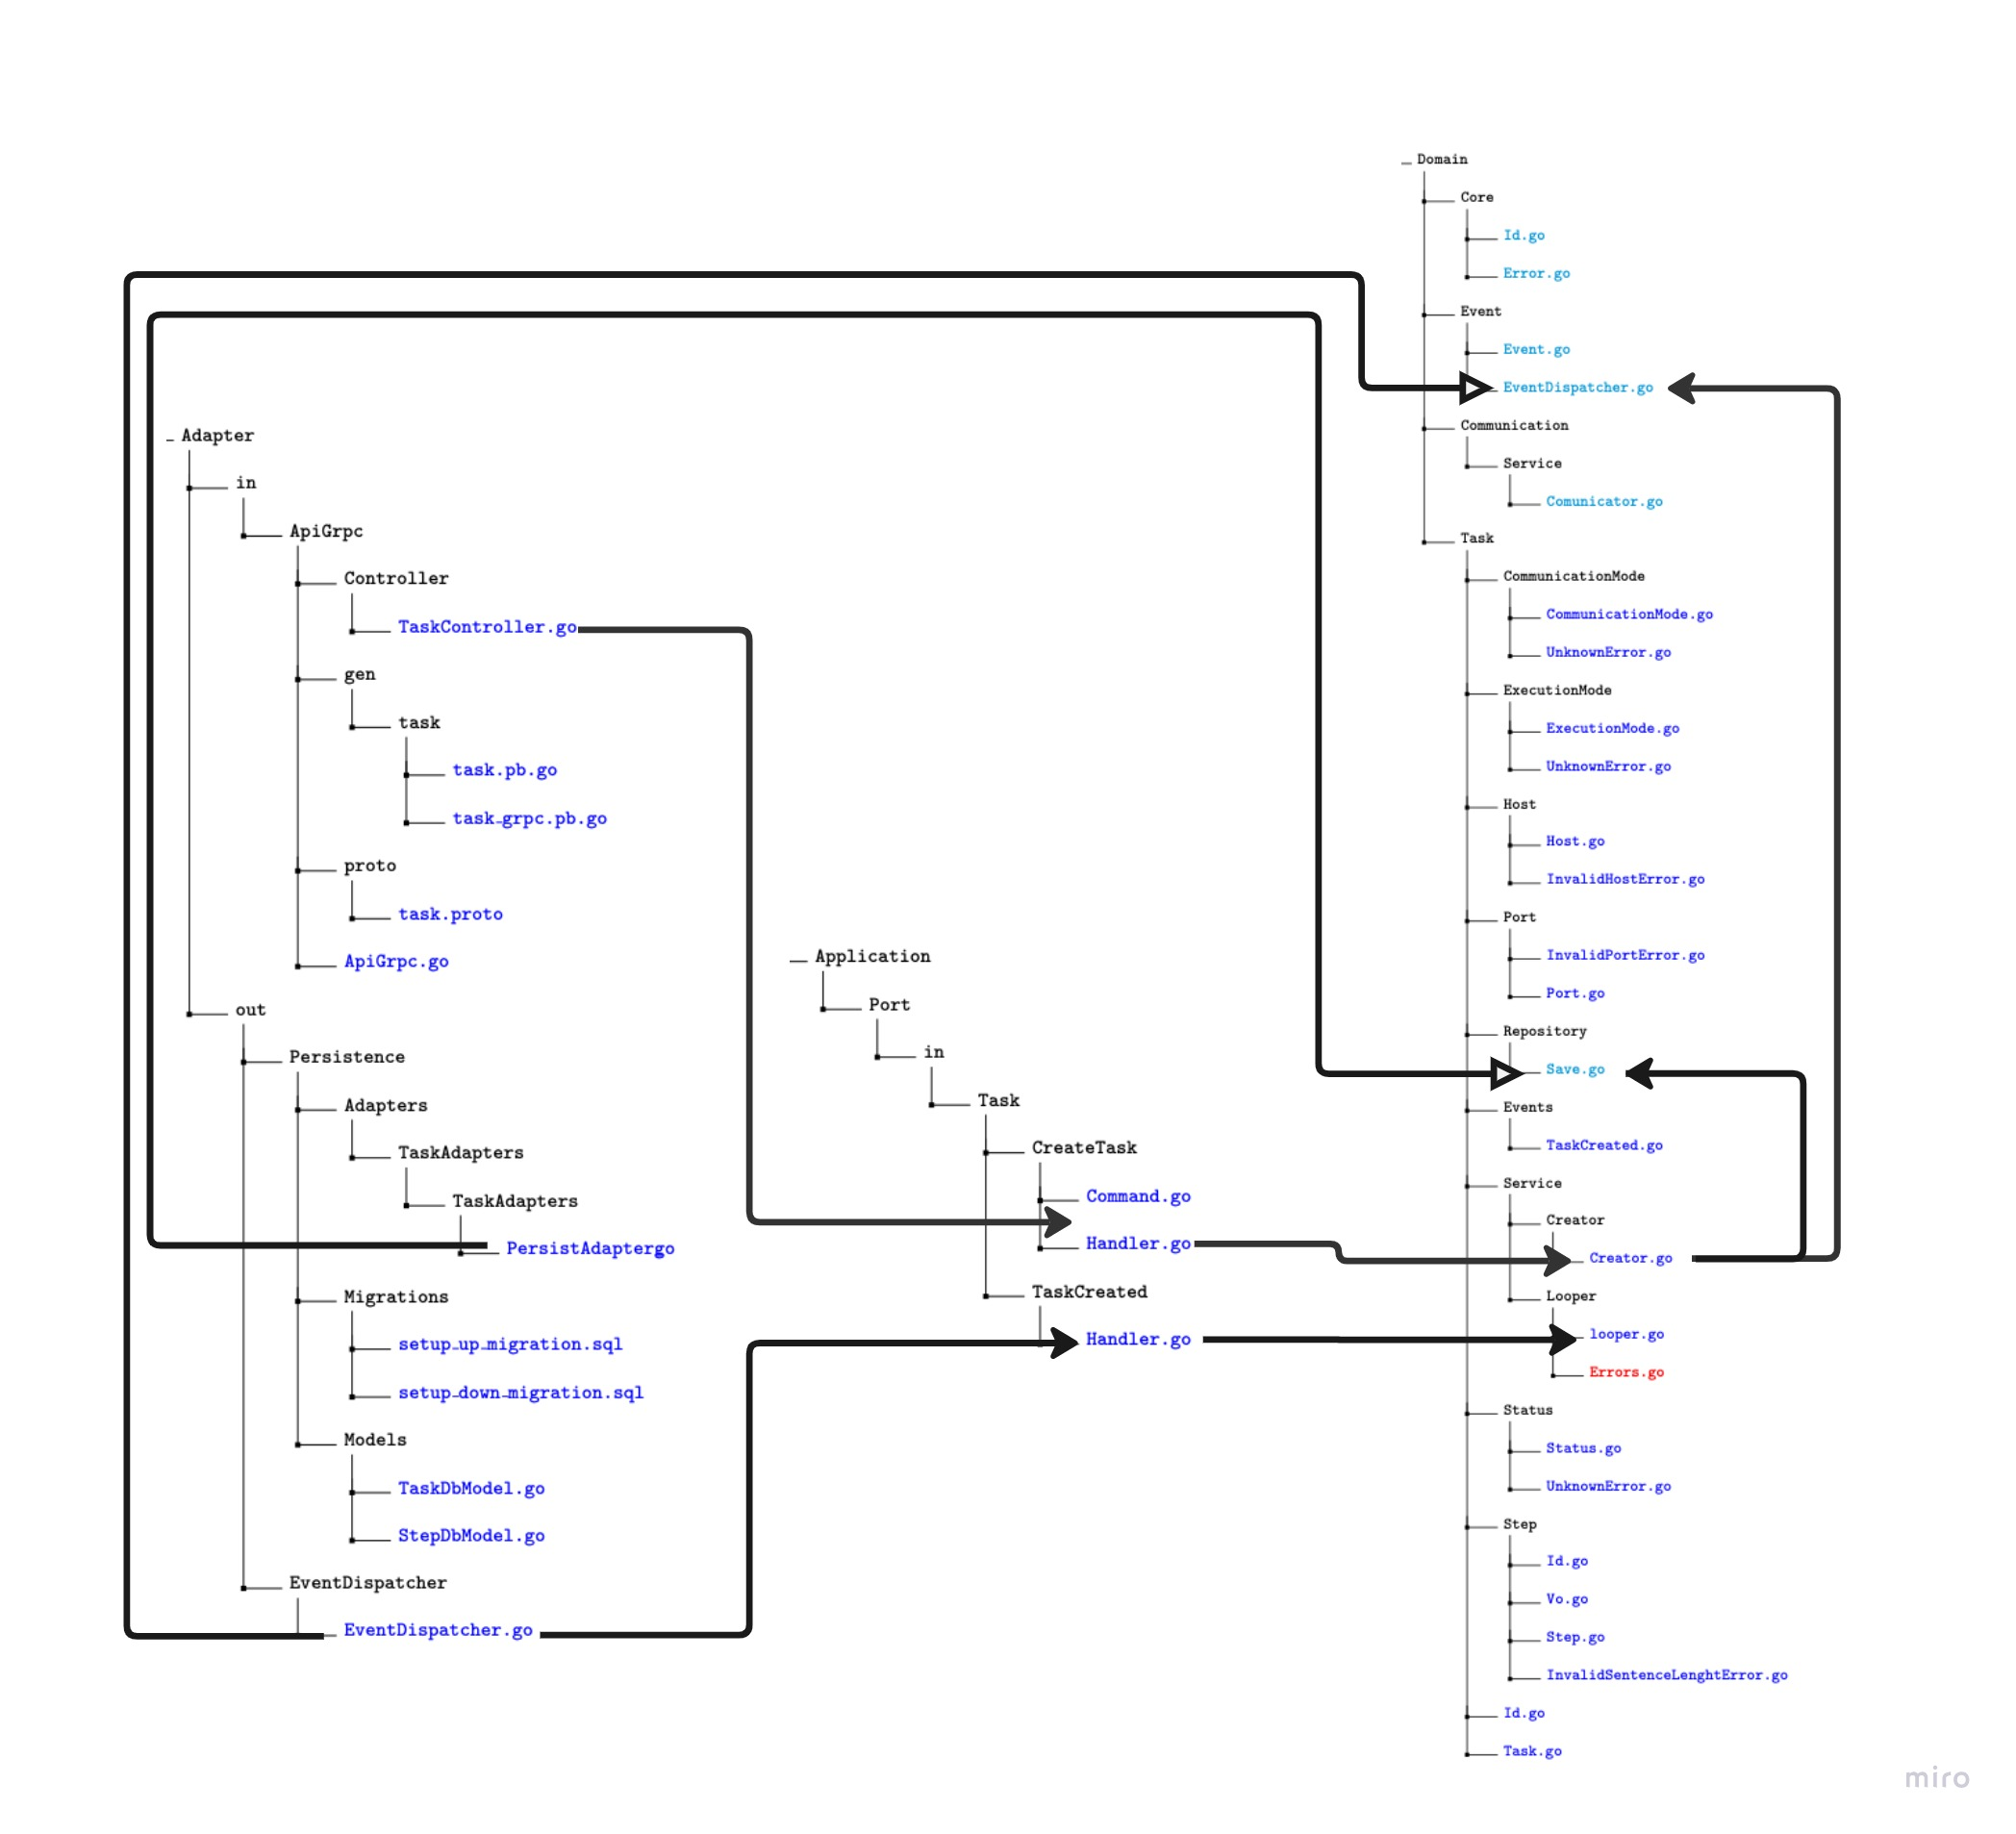
\includegraphics[height=0.5\textheight]{./part/Ejecucion/Seguimiento/CreateTaskUseCase/img/PFM - CreateUseCaseFolderStructure}
    \caption{CreateTaskUseCase folder Structure}\label{fig:createTaskUseCaseArchitectureFolderStructure}
\end{figure}

%Un punto interesante a comentar es el concepto de la estrategia de mapping que hay entre capas. Cada capa requiere sus objetos de trabajo. Tal y como sale descrito en \cite{TomHombergs2019GYHD} Tenemos tantas estratégias como atajos dentro de este paradigma queramos asumir. podemos ver en la figura \ref{fig:mapping types} Los tipos de mapping que se documentan en este libro:
%\begin{itemize}
%    \item The NoMapping Strategy
%    \item The Two-Way MappingStrategy
%    \item The Full MappingStrategy
%    \item The One-Way MappingStrategy
%\end{itemize}

Con respecto a la estrategia de mapping Golang nos permite hacer un full strategy casi por defecto porque al necesitar la implementaci'on de clase para garantizar la cohesión ya estamos utilizando interfaces para todas las clases. Así que en este caso utilizamos un fullMapping adaptado. lo cierto es que las versiones intermedias son todas las combinaciones posibles.

De cara a decidir extraemos la recomendacion de  \cite{TomHombergs2019GYHD}:"
we might start with a simple strategy that allows us to quickly evolve the code and later move to a more complex one that helps us to better decouple the layers.
In order to decide which strategy to use when, we need to agree upon a set of guidelines within the team. These guidelines should answer the question which mapping strategy should be the first choice in which situation. They should also answer why they are first choice so that we’re able to evaluate if those reasons still apply after some time."

Al final se trata de tomar una decisión en equipo, documentar las razones y ser consistentes. Reevaluar las razones ante un reto que las ponga a prueba y tomar o no la decisión de cambiar la estrategia.

En nuestra opinión dentro de la estrategia fullmapping se debe implementar un modelo tanto de entrada, como ya se contempla, como de salída. Es decir, la respuesta que hay entre cada capa también debe ser mappeada, podemos ver el patrón readptado en la figura \ref{fig:GetHandMapping}

\begin{figure}[H]
    \centering
    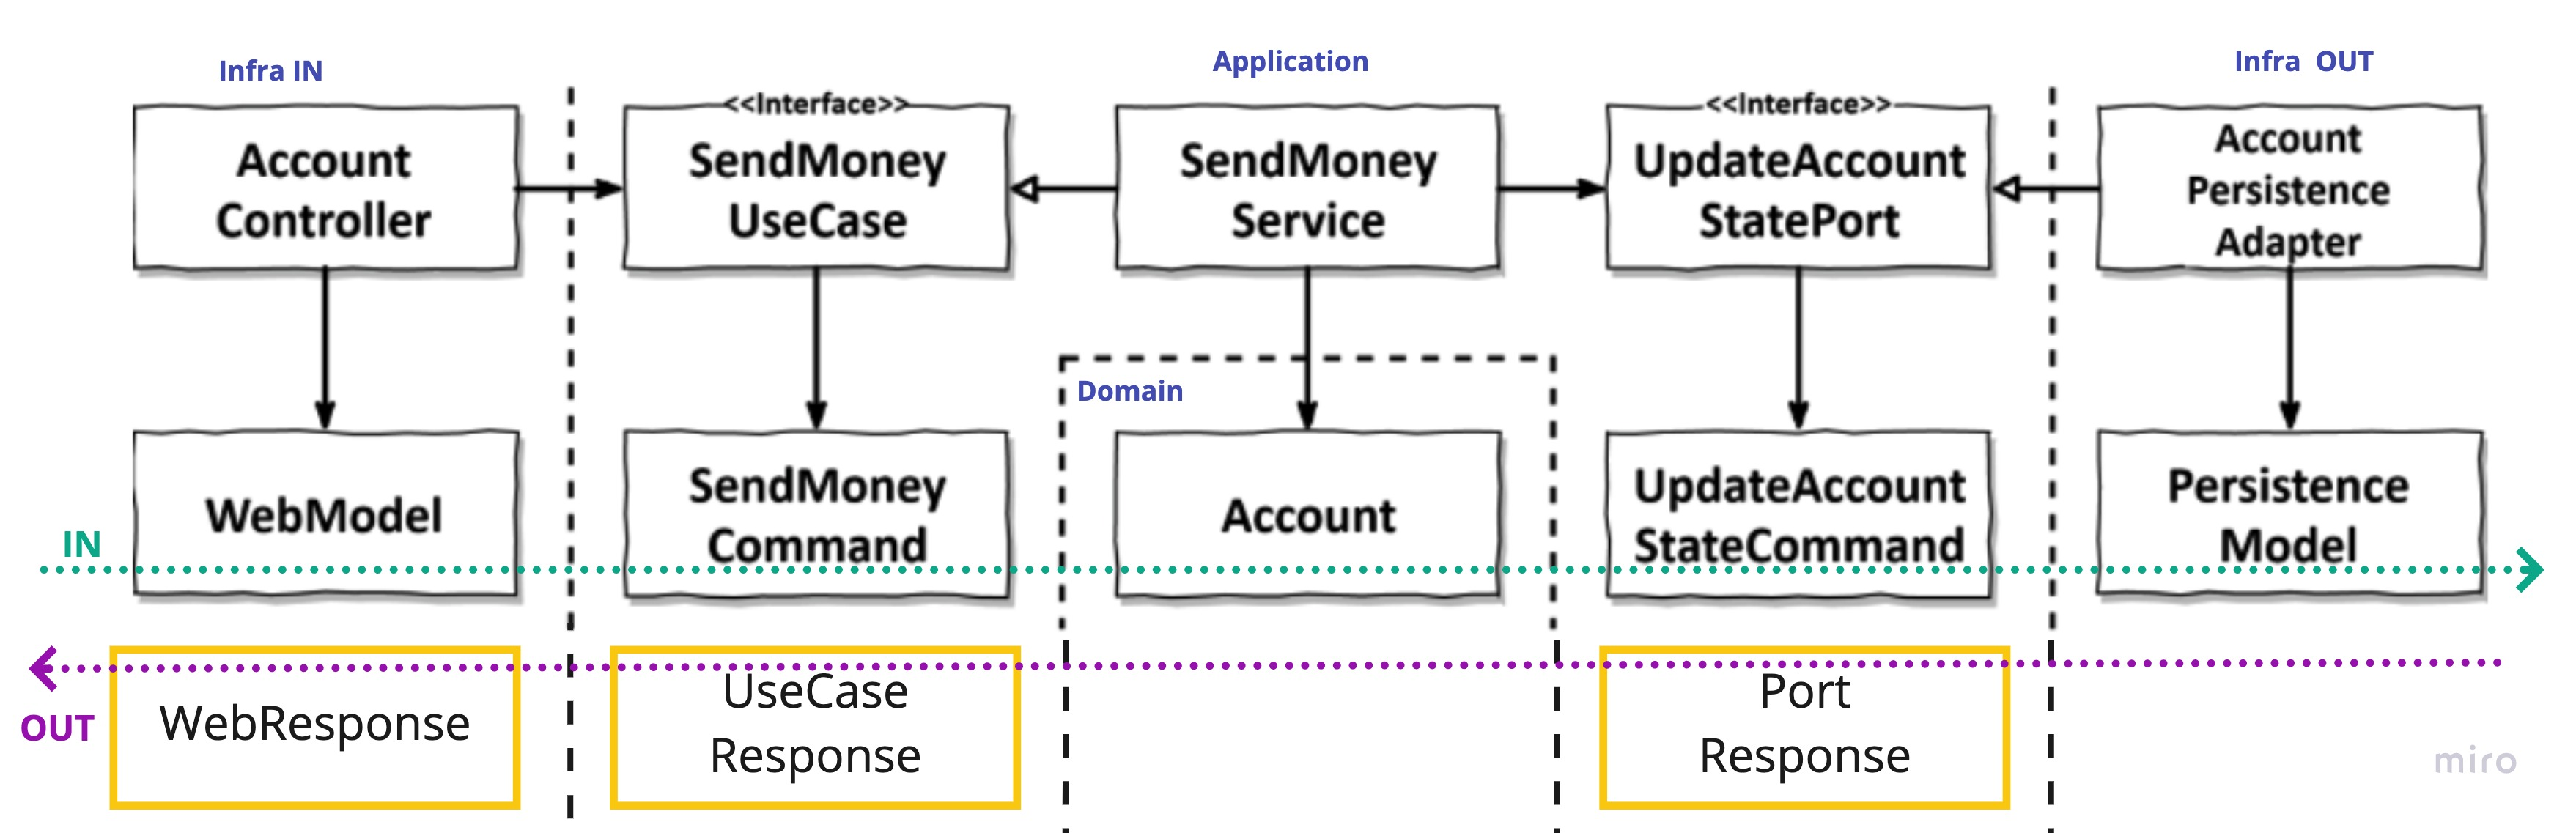
\includegraphics[height=0.2\textheight]{./part/Ejecucion/Seguimiento/CreateTaskUseCase/img/PFM - GetHandMapping}
    \caption{CreateTaskUseCase folder Structure\cite{TomHombergs2019GYHD}}\label{fig:GetHandMapping}
\end{figure}

Claramente esto aumenta la burocracia y finalmente la opción que hemos tomado se puede ver en la figura\ref{fig:CreateTaskUseCaseMapping}

En rojo se han marcado los atajos que se han tomado, es decir, el mapeo que no se ha implementado. El objetivo es aislarse bien de los puertos de entrada, es decir el GRPC, y no tanto de los puertos de salida. ya que la persistencia está bien aislada mediante las interfaces. Dentro de los adaptadores se hará el trabajo de mappeo entre las entidades de dominio y los modelos de persistencia y se traducirá de nuevo a dominio para responder.

\begin{figure}[H]
    \centering
    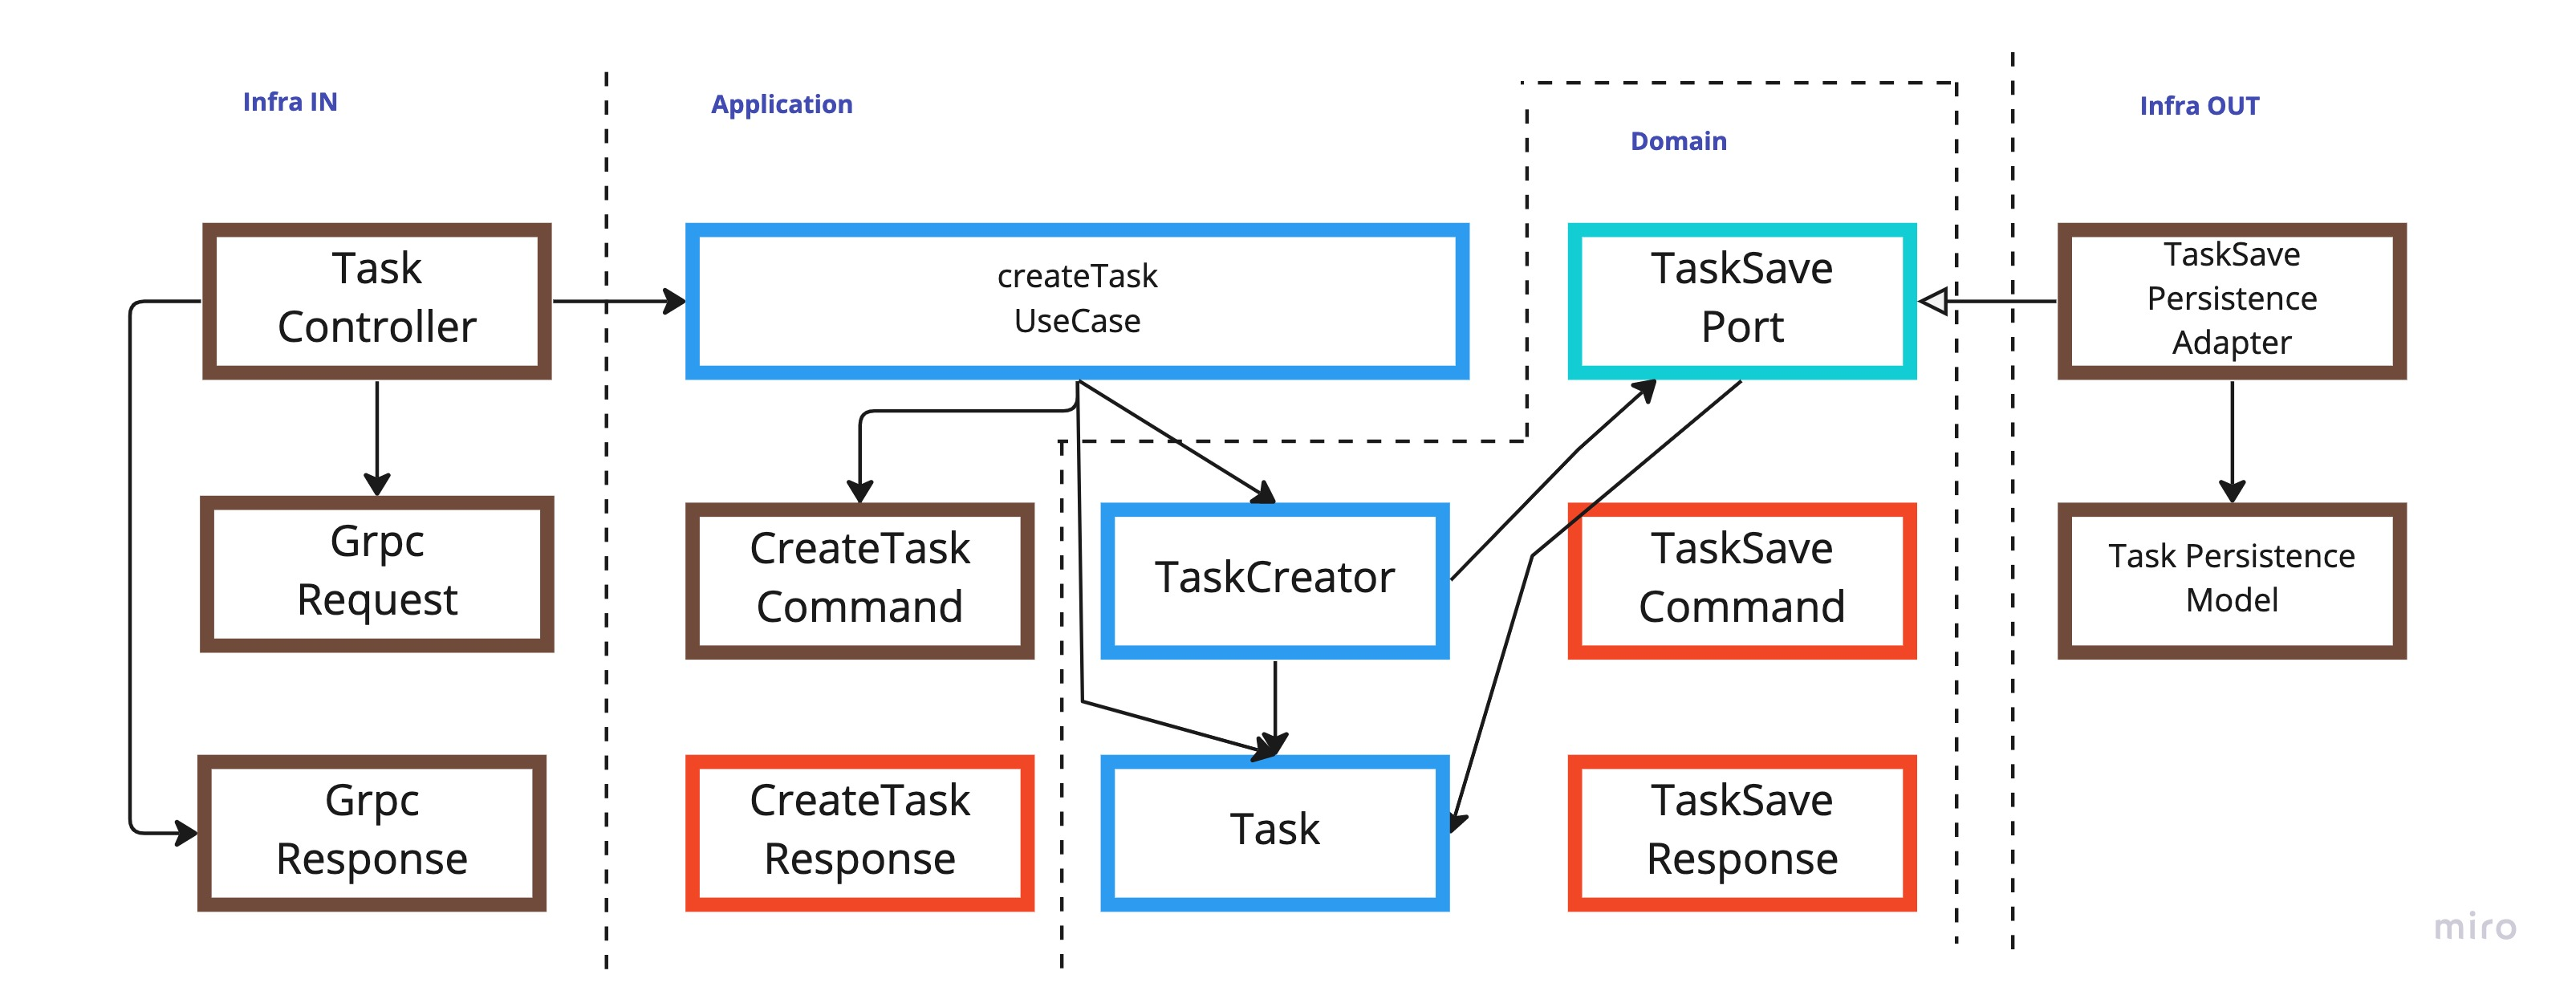
\includegraphics[height=0.2\textheight]{./part/Ejecucion/Seguimiento/CreateTaskUseCase/img/PFM - FinalMapping}
    \caption{CreateTaskUseCase folder Structure}\label{fig:CreateTaskUseCaseMapping}
\end{figure}

Ahora vamos a exponer el código final de este caso de uso, vamos a hacer referencia a:
\begin{itemize}
    \item TaskController \ref{fig:TaskControler}
    \item CreateTaskUseCase \ref{fig:CreateTaskUseCaseCode}
    \item Creator \ref{fig:Creator}
    \item SavePort \ref{fig:SavePort}
    \item PersistAdapter \ref{fig:SaveAdapter}
    \item DispatcherPort \ref{fig:DispatcherPort}
\end{itemize}

\begin{figure}[H]
    \centering
    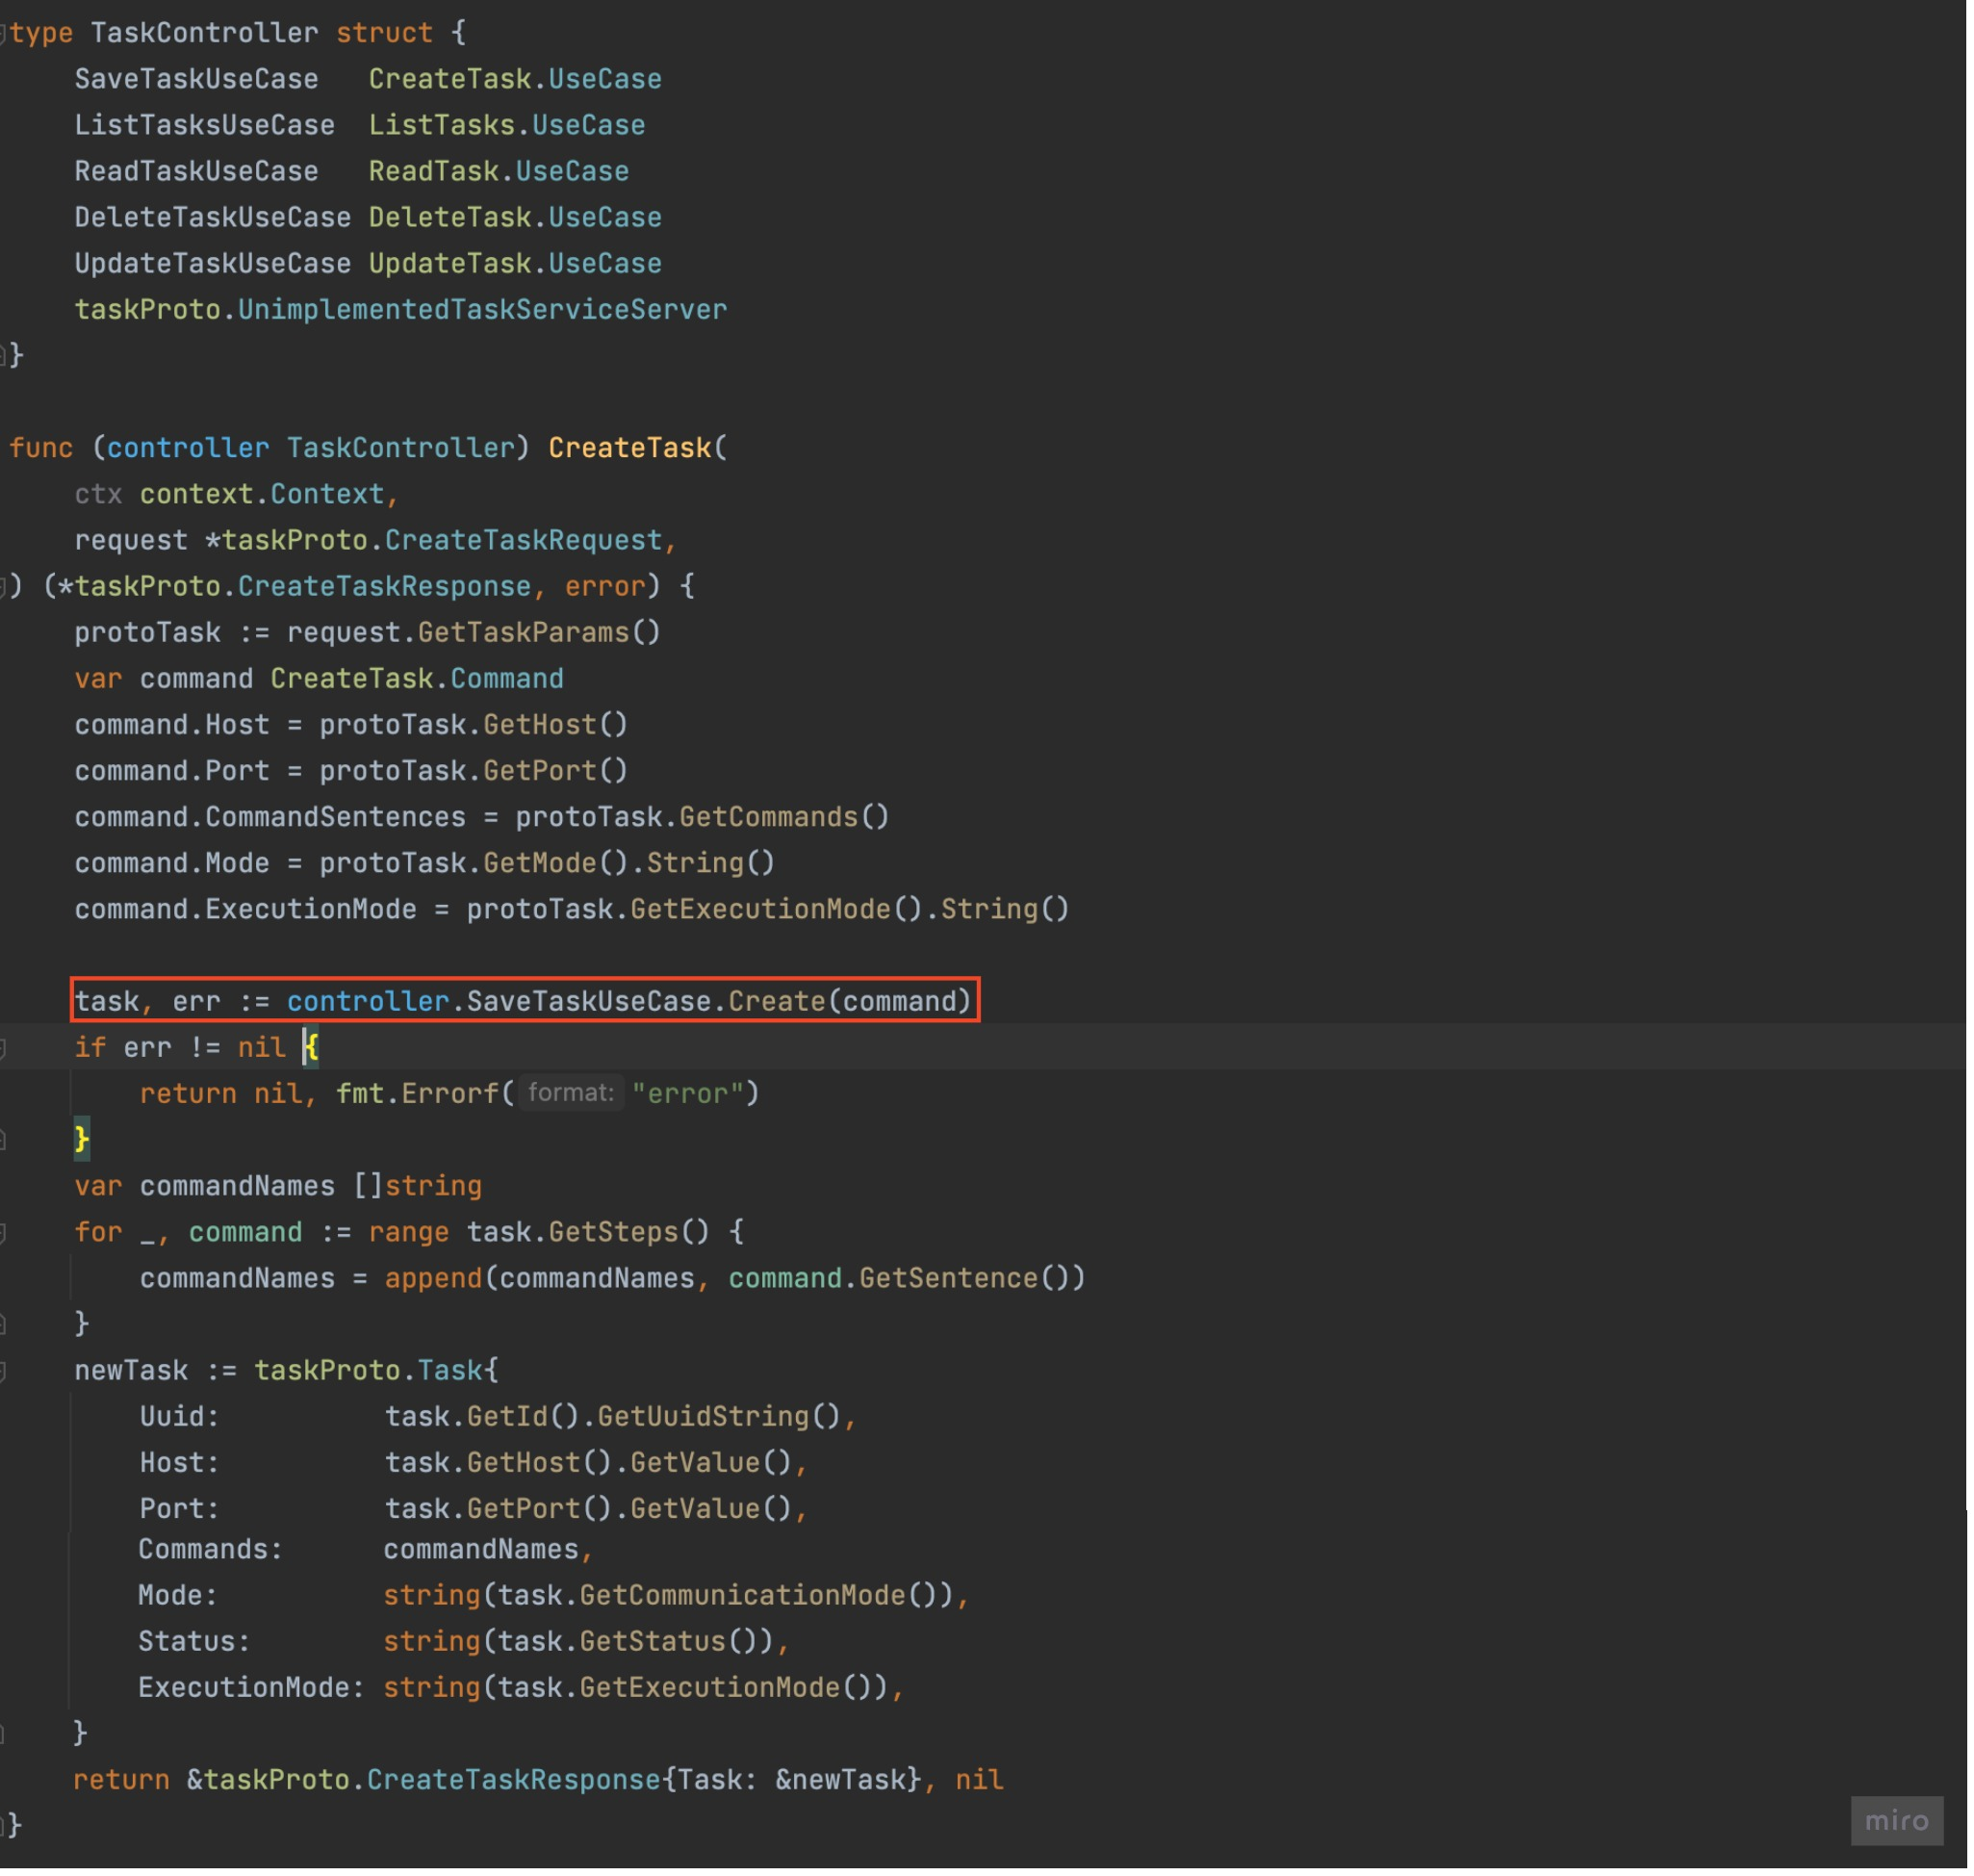
\includegraphics[height=0.5\textheight]{./part/Ejecucion/Seguimiento/CreateTaskUseCase/img/PFM - TaskController}
    \caption{TaskController.go}\label{fig:TaskControler}
\end{figure}

\begin{figure}[H]
    \centering
    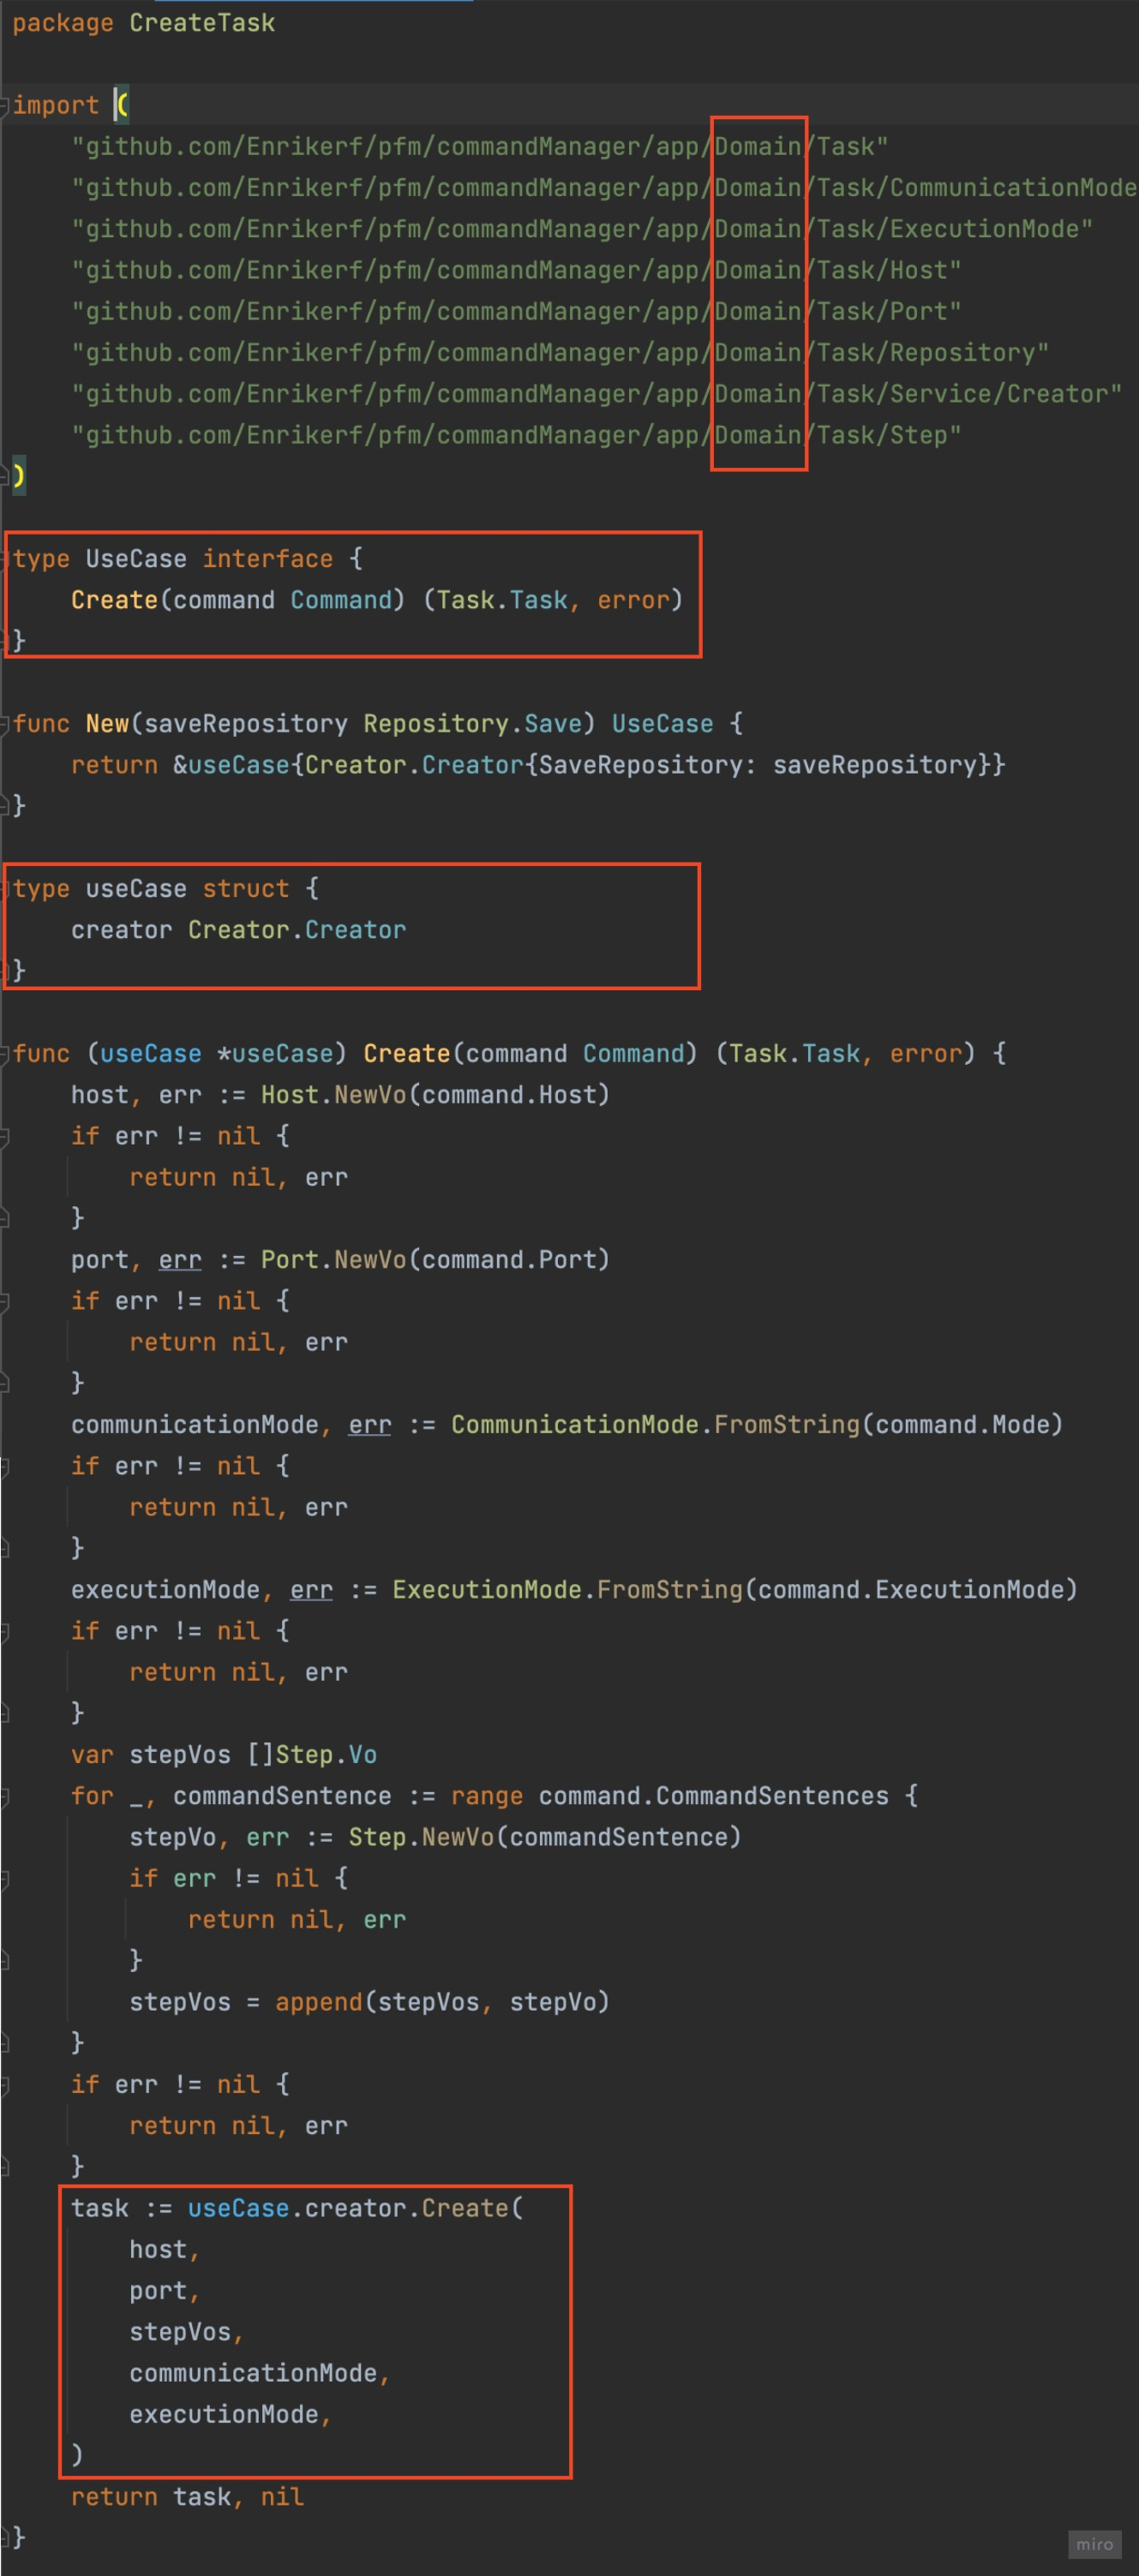
\includegraphics[height=0.5\textheight]{./part/Ejecucion/Seguimiento/CreateTaskUseCase/img/PFM - CreateTaskUseCaseCode}
    \caption{CreateTaskUseCaseCode.go}\label{fig:CreateTaskUseCaseCode}
\end{figure}

\begin{figure}[H]
    \centering
    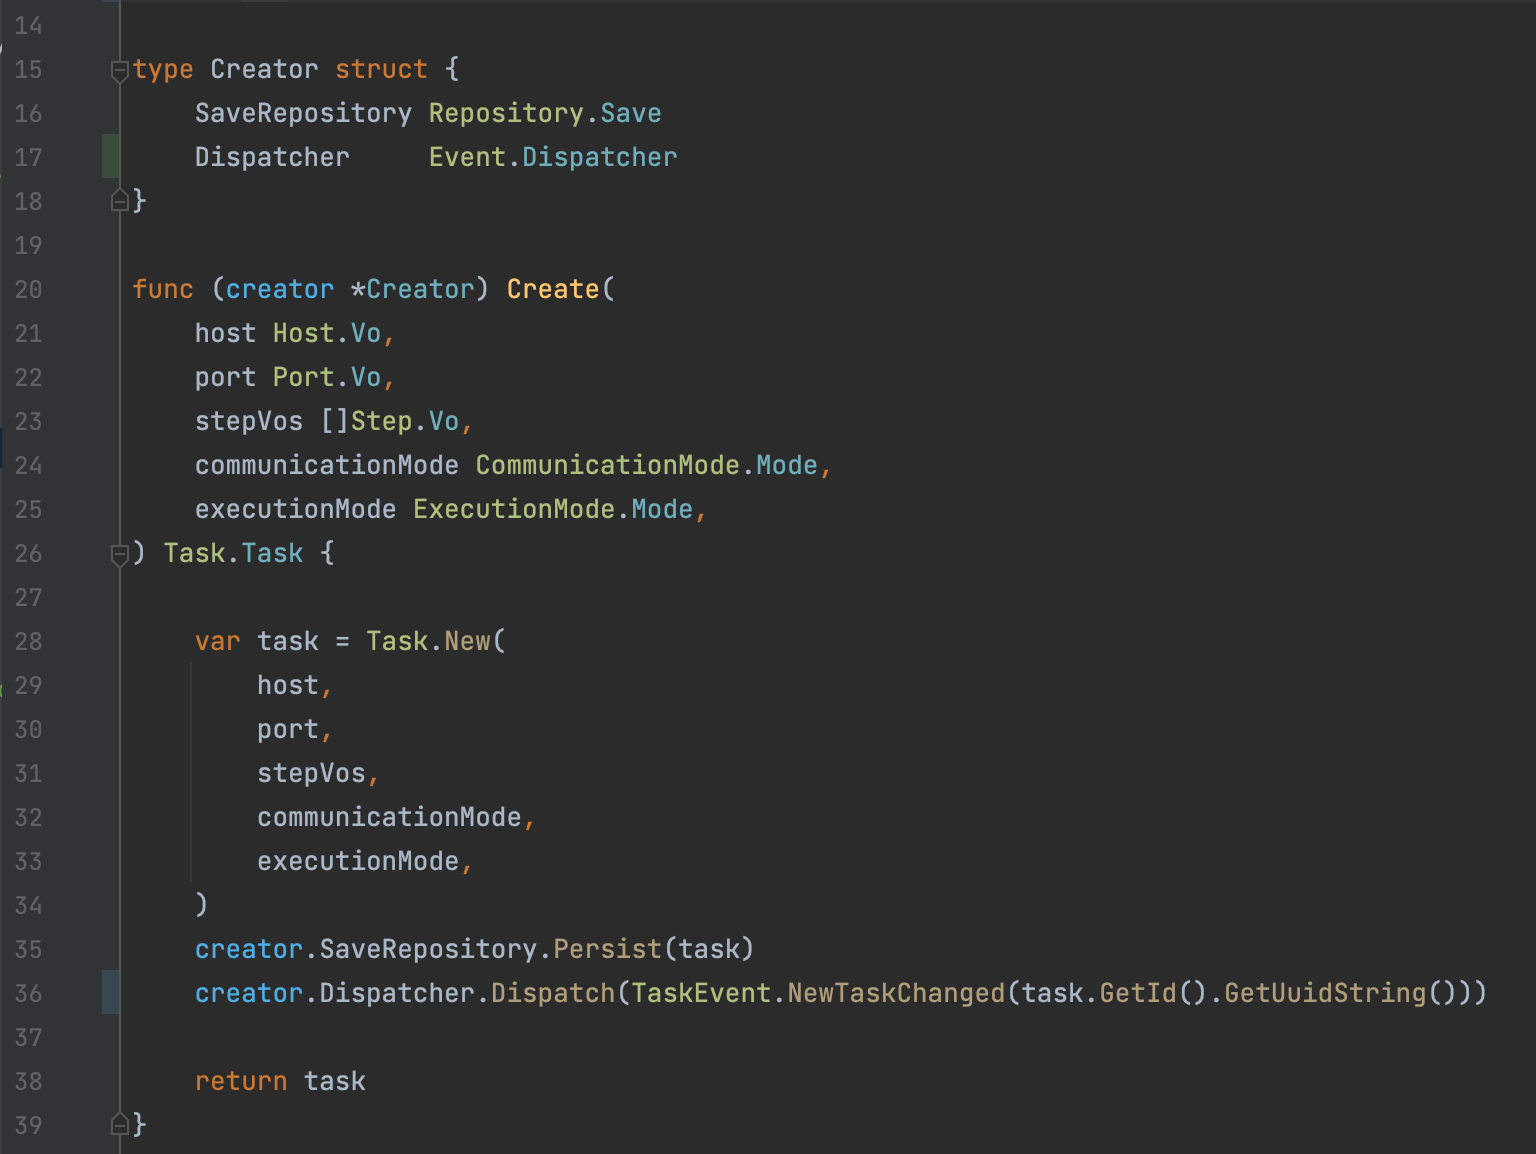
\includegraphics[height=0.5\textheight]{./part/Ejecucion/Seguimiento/CreateTaskUseCase/img/PFM - creator}
    \caption{Creator.go}\label{fig:Creator}
\end{figure}

\begin{figure}[H]
    \centering
    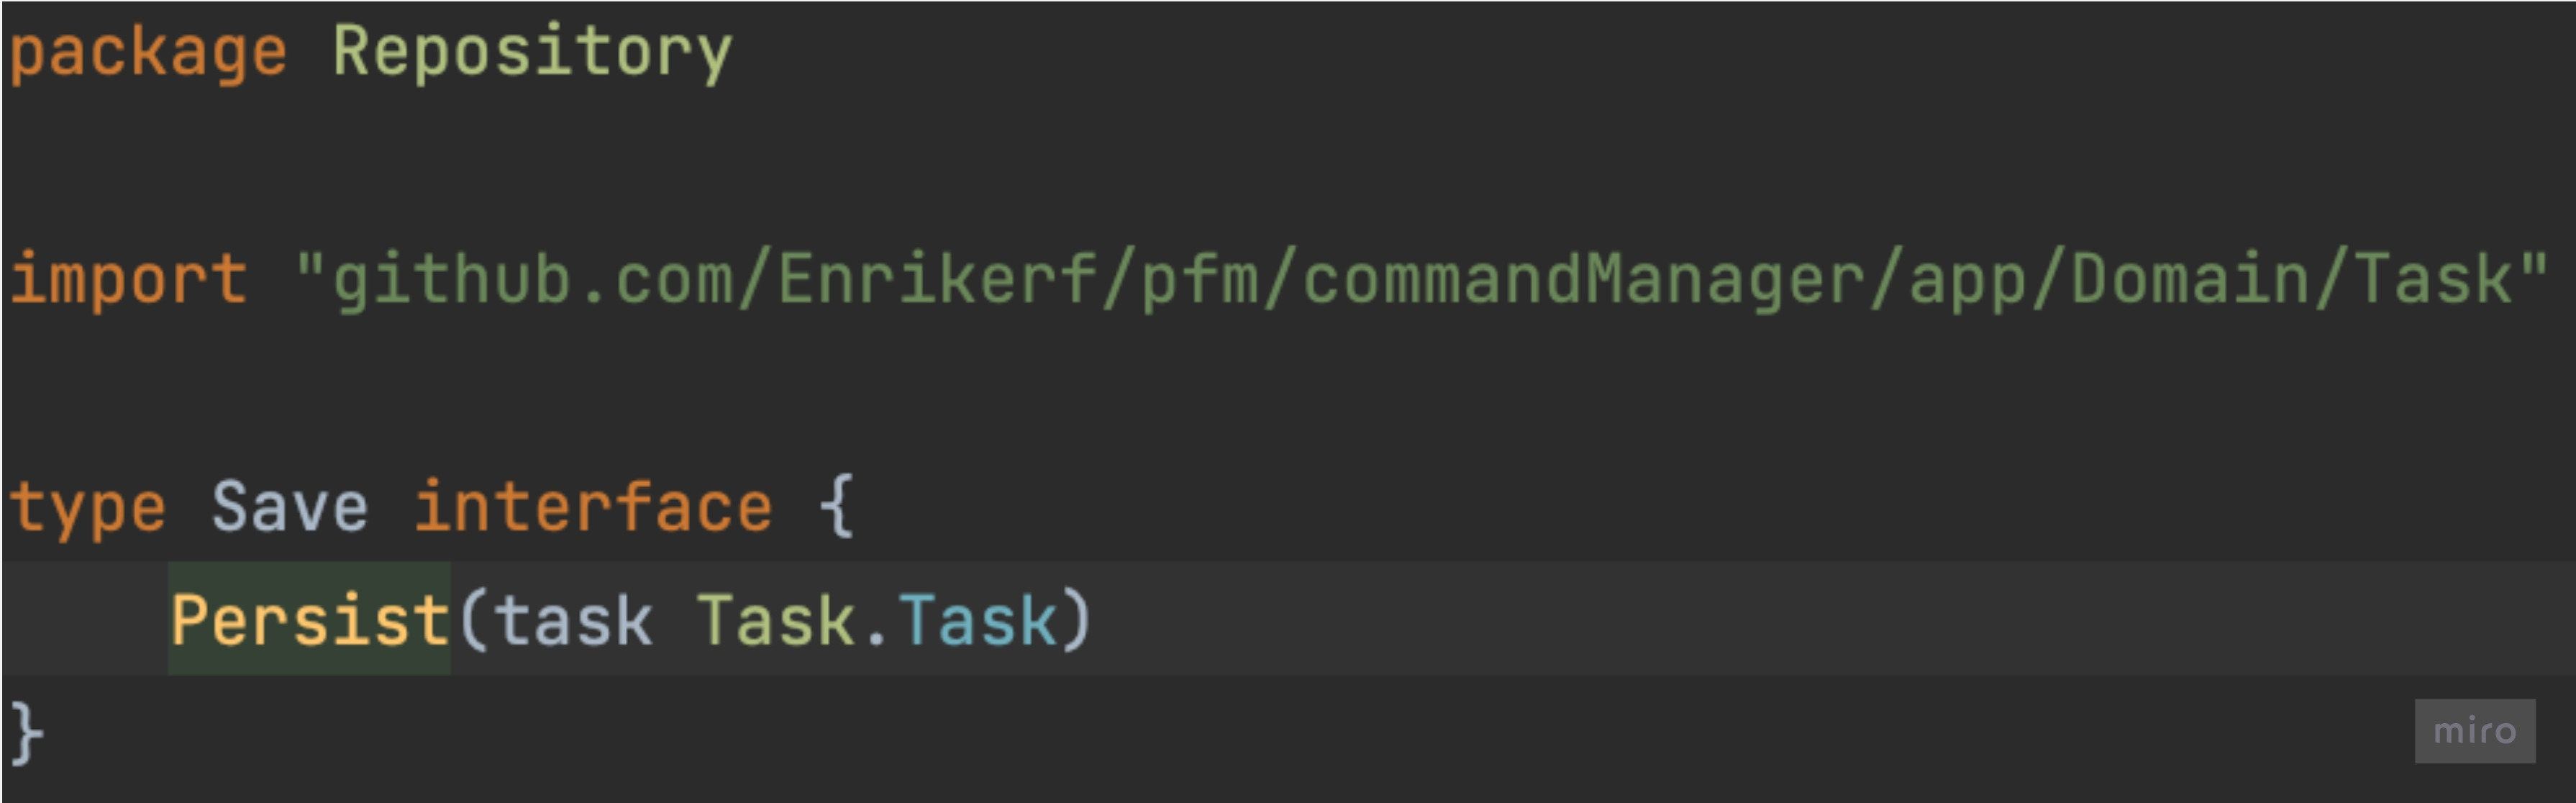
\includegraphics[height=0.2\textheight]{./part/Ejecucion/Seguimiento/CreateTaskUseCase/img/PFM - SavePort}
    \caption{Creator.go}\label{fig:SavePort}
\end{figure}

\begin{figure}[H]
    \centering
    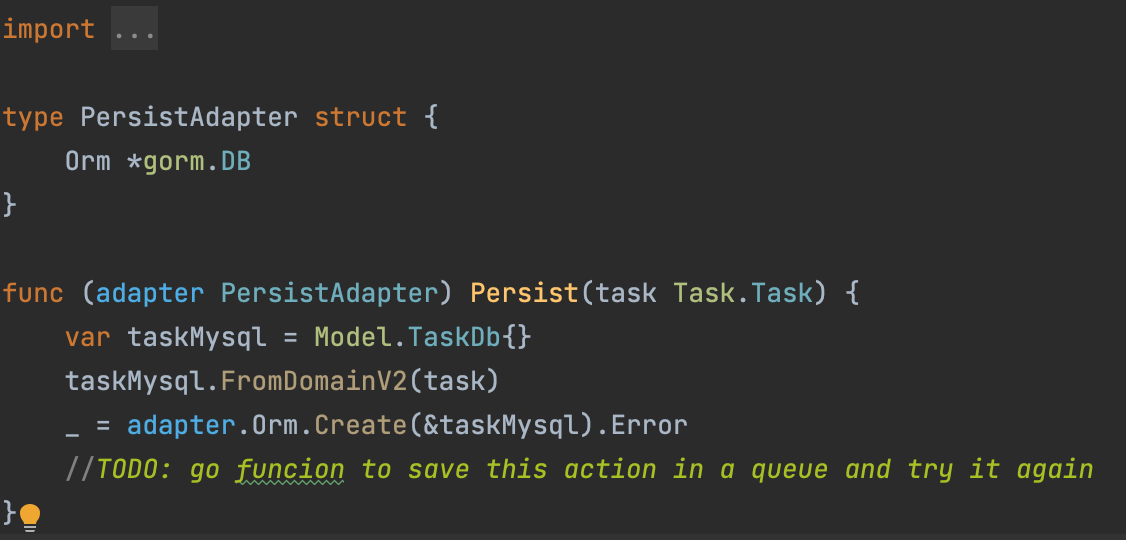
\includegraphics[height=0.2\textheight]{./part/Ejecucion/Seguimiento/CreateTaskUseCase/img/PFM - SaveAdapter}
    \caption{Creator.go}\label{fig:SaveAdapter}
\end{figure}

\begin{figure}[H]
    \centering
    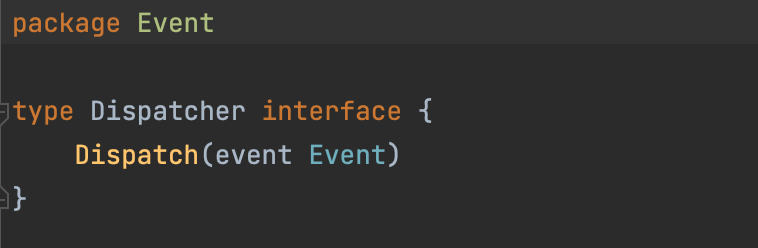
\includegraphics[height=0.2\textheight]{./part/Ejecucion/Seguimiento/CreateTaskUseCase/img/PFM - Dispatcher}
    \caption{Creator.go}\label{fig:DispatcherPort}
\end{figure}
\subsubsection{Asincronía}\label{subsec:asincronia}
    \paragraph{Encoder}
    \paragraph{RPC Server streaming}
    \paragraph{RPC Bidirectional}
\subsubsection{Testing}
\subsubsection{Puesta a punto y resultados}